% Options for packages loaded elsewhere
\PassOptionsToPackage{unicode}{hyperref}
\PassOptionsToPackage{hyphens}{url}
\documentclass[
]{book}
\usepackage{xcolor}
\usepackage{amsmath,amssymb}
\setcounter{secnumdepth}{5}
\usepackage{iftex}
\ifPDFTeX
  \usepackage[T1]{fontenc}
  \usepackage[utf8]{inputenc}
  \usepackage{textcomp} % provide euro and other symbols
\else % if luatex or xetex
  \usepackage{unicode-math} % this also loads fontspec
  \defaultfontfeatures{Scale=MatchLowercase}
  \defaultfontfeatures[\rmfamily]{Ligatures=TeX,Scale=1}
\fi
\usepackage{lmodern}
\ifPDFTeX\else
  % xetex/luatex font selection
\fi
% Use upquote if available, for straight quotes in verbatim environments
\IfFileExists{upquote.sty}{\usepackage{upquote}}{}
\IfFileExists{microtype.sty}{% use microtype if available
  \usepackage[]{microtype}
  \UseMicrotypeSet[protrusion]{basicmath} % disable protrusion for tt fonts
}{}
\makeatletter
\@ifundefined{KOMAClassName}{% if non-KOMA class
  \IfFileExists{parskip.sty}{%
    \usepackage{parskip}
  }{% else
    \setlength{\parindent}{0pt}
    \setlength{\parskip}{6pt plus 2pt minus 1pt}}
}{% if KOMA class
  \KOMAoptions{parskip=half}}
\makeatother
\usepackage{color}
\usepackage{fancyvrb}
\newcommand{\VerbBar}{|}
\newcommand{\VERB}{\Verb[commandchars=\\\{\}]}
\DefineVerbatimEnvironment{Highlighting}{Verbatim}{commandchars=\\\{\}}
% Add ',fontsize=\small' for more characters per line
\usepackage{framed}
\definecolor{shadecolor}{RGB}{248,248,248}
\newenvironment{Shaded}{\begin{snugshade}}{\end{snugshade}}
\newcommand{\AlertTok}[1]{\textcolor[rgb]{0.94,0.16,0.16}{#1}}
\newcommand{\AnnotationTok}[1]{\textcolor[rgb]{0.56,0.35,0.01}{\textbf{\textit{#1}}}}
\newcommand{\AttributeTok}[1]{\textcolor[rgb]{0.13,0.29,0.53}{#1}}
\newcommand{\BaseNTok}[1]{\textcolor[rgb]{0.00,0.00,0.81}{#1}}
\newcommand{\BuiltInTok}[1]{#1}
\newcommand{\CharTok}[1]{\textcolor[rgb]{0.31,0.60,0.02}{#1}}
\newcommand{\CommentTok}[1]{\textcolor[rgb]{0.56,0.35,0.01}{\textit{#1}}}
\newcommand{\CommentVarTok}[1]{\textcolor[rgb]{0.56,0.35,0.01}{\textbf{\textit{#1}}}}
\newcommand{\ConstantTok}[1]{\textcolor[rgb]{0.56,0.35,0.01}{#1}}
\newcommand{\ControlFlowTok}[1]{\textcolor[rgb]{0.13,0.29,0.53}{\textbf{#1}}}
\newcommand{\DataTypeTok}[1]{\textcolor[rgb]{0.13,0.29,0.53}{#1}}
\newcommand{\DecValTok}[1]{\textcolor[rgb]{0.00,0.00,0.81}{#1}}
\newcommand{\DocumentationTok}[1]{\textcolor[rgb]{0.56,0.35,0.01}{\textbf{\textit{#1}}}}
\newcommand{\ErrorTok}[1]{\textcolor[rgb]{0.64,0.00,0.00}{\textbf{#1}}}
\newcommand{\ExtensionTok}[1]{#1}
\newcommand{\FloatTok}[1]{\textcolor[rgb]{0.00,0.00,0.81}{#1}}
\newcommand{\FunctionTok}[1]{\textcolor[rgb]{0.13,0.29,0.53}{\textbf{#1}}}
\newcommand{\ImportTok}[1]{#1}
\newcommand{\InformationTok}[1]{\textcolor[rgb]{0.56,0.35,0.01}{\textbf{\textit{#1}}}}
\newcommand{\KeywordTok}[1]{\textcolor[rgb]{0.13,0.29,0.53}{\textbf{#1}}}
\newcommand{\NormalTok}[1]{#1}
\newcommand{\OperatorTok}[1]{\textcolor[rgb]{0.81,0.36,0.00}{\textbf{#1}}}
\newcommand{\OtherTok}[1]{\textcolor[rgb]{0.56,0.35,0.01}{#1}}
\newcommand{\PreprocessorTok}[1]{\textcolor[rgb]{0.56,0.35,0.01}{\textit{#1}}}
\newcommand{\RegionMarkerTok}[1]{#1}
\newcommand{\SpecialCharTok}[1]{\textcolor[rgb]{0.81,0.36,0.00}{\textbf{#1}}}
\newcommand{\SpecialStringTok}[1]{\textcolor[rgb]{0.31,0.60,0.02}{#1}}
\newcommand{\StringTok}[1]{\textcolor[rgb]{0.31,0.60,0.02}{#1}}
\newcommand{\VariableTok}[1]{\textcolor[rgb]{0.00,0.00,0.00}{#1}}
\newcommand{\VerbatimStringTok}[1]{\textcolor[rgb]{0.31,0.60,0.02}{#1}}
\newcommand{\WarningTok}[1]{\textcolor[rgb]{0.56,0.35,0.01}{\textbf{\textit{#1}}}}
\usepackage{longtable,booktabs,array}
\usepackage{calc} % for calculating minipage widths
% Correct order of tables after \paragraph or \subparagraph
\usepackage{etoolbox}
\makeatletter
\patchcmd\longtable{\par}{\if@noskipsec\mbox{}\fi\par}{}{}
\makeatother
% Allow footnotes in longtable head/foot
\IfFileExists{footnotehyper.sty}{\usepackage{footnotehyper}}{\usepackage{footnote}}
\makesavenoteenv{longtable}
\usepackage{graphicx}
\makeatletter
\newsavebox\pandoc@box
\newcommand*\pandocbounded[1]{% scales image to fit in text height/width
  \sbox\pandoc@box{#1}%
  \Gscale@div\@tempa{\textheight}{\dimexpr\ht\pandoc@box+\dp\pandoc@box\relax}%
  \Gscale@div\@tempb{\linewidth}{\wd\pandoc@box}%
  \ifdim\@tempb\p@<\@tempa\p@\let\@tempa\@tempb\fi% select the smaller of both
  \ifdim\@tempa\p@<\p@\scalebox{\@tempa}{\usebox\pandoc@box}%
  \else\usebox{\pandoc@box}%
  \fi%
}
% Set default figure placement to htbp
\def\fps@figure{htbp}
\makeatother
\setlength{\emergencystretch}{3em} % prevent overfull lines
\providecommand{\tightlist}{%
  \setlength{\itemsep}{0pt}\setlength{\parskip}{0pt}}
\usepackage[]{natbib}
\bibliographystyle{plainnat}
\usepackage{booktabs}
\usepackage{bookmark}
\IfFileExists{xurl.sty}{\usepackage{xurl}}{} % add URL line breaks if available
\urlstyle{same}
\hypersetup{
  pdftitle={Week 9: Logit and Probit},
  pdfauthor={Samuel Rowe adapted from Wooldridge (2011), Long and Freese (2006), and Mitchell (2020)},
  hidelinks,
  pdfcreator={LaTeX via pandoc}}

\title{Week 9: Logit and Probit}
\author{Samuel Rowe adapted from Wooldridge (2011), Long and Freese (2006), and Mitchell (2020)}
\date{2025-11-05}

\begin{document}
\maketitle

{
\setcounter{tocdepth}{1}
\tableofcontents
}
\begin{Shaded}
\begin{Highlighting}[]
\NormalTok{bookdown}\SpecialCharTok{::}\FunctionTok{render\_book}\NormalTok{()}
\end{Highlighting}
\end{Shaded}

\chapter*{Overview}\label{overview}
\addcontentsline{toc}{chapter}{Overview}

We will cover the implementation of logit, probit, and multinomial logit.

\begin{enumerate}
\def\labelenumi{\arabic{enumi}.}
\tightlist
\item
  Logit, Probit, and Linear Probability Model
\item
  Multinomial Logit
\item
  Ordinal Logit
\item
  Reshape
\end{enumerate}

\chapter{Binary Outcomes}\label{binary-outcomes}

\section*{Married Women's Labor Force Participation}\label{married-womens-labor-force-participation}
\addcontentsline{toc}{section}{Married Women's Labor Force Participation}

\begin{Shaded}
\begin{Highlighting}[]
\NormalTok{cd }\StringTok{"/Users/Sam/Desktop/Econ 645/Data/Wooldridge"}
\KeywordTok{use}\NormalTok{ mroz.dta, }\KeywordTok{clear}
\end{Highlighting}
\end{Shaded}

We'll use the data from Mroz (1987) to look at the probability of a married woman being in the labor force. Labor force participation is a binary response.

\[ y=[0,1] \]
We will estimate the coefficients of the linear probability model (LPM), the logit estimator, and the probit estimator. Then, we'll compare the marginal effects ofall three estimators.

Summarize in the labor force

\begin{Shaded}
\begin{Highlighting}[]
\KeywordTok{tabulate}\NormalTok{ inlf}
\end{Highlighting}
\end{Shaded}

\begin{verbatim}
       inlf |      Freq.     Percent        Cum.
------------+-----------------------------------
          0 |        325       43.16       43.16
          1 |        428       56.84      100.00
------------+-----------------------------------
      Total |        753      100.00
\end{verbatim}

There are 325 women are not in the labor force and 428 women participating in the labor force.
Our explanatory variables are non-wife income, education, experience, experience-squared, age, kids less than 6, kids greater than 6

\[ y_{i}=\beta_0 + \beta_1 spouseinc_{i} + \beta_2 edu_i + \beta_3 exp_i + \beta_4 exp^2_i + \beta_5 kidsLT6_i + \beta_6 kidsGT6_i + \varepsilon_i  \]

\begin{Shaded}
\begin{Highlighting}[]
\KeywordTok{est} \KeywordTok{clear}
\NormalTok{eststo Logit: }\KeywordTok{logit}\NormalTok{ inlf nwifeinc educ exper expersq kidslt6 kidsge6}
\NormalTok{eststo Probit: }\KeywordTok{probit}\NormalTok{ inlf nwifeinc educ exper expersq kidslt6 kidsge6}
\NormalTok{esttab Logit Probit, mtitle}
\end{Highlighting}
\end{Shaded}

\begin{verbatim}
Iteration 0:   log likelihood =  -514.8732  
Iteration 1:   log likelihood = -422.78042  
Iteration 2:   log likelihood = -421.73851  
Iteration 3:   log likelihood = -421.73502  
Iteration 4:   log likelihood = -421.73502  

Logistic regression                             Number of obs     =        753
                                                LR chi2(6)        =     186.28
                                                Prob > chi2       =     0.0000
Log likelihood = -421.73502                     Pseudo R2         =     0.1809

------------------------------------------------------------------------------
        inlf |      Coef.   Std. Err.      z    P>|z|     [95% Conf. Interval]
-------------+----------------------------------------------------------------
    nwifeinc |  -.0301171   .0082431    -3.65   0.000    -.0462734   -.0139609
        educ |   .2520038   .0425492     5.92   0.000      .168609    .3353987
       exper |   .2057387   .0310518     6.63   0.000     .1448784     .266599
     expersq |   -.003913   .0009994    -3.92   0.000    -.0058718   -.0019541
     kidslt6 |  -.9175126   .1742458    -5.27   0.000    -1.259028   -.5759971
     kidsge6 |   .2226164   .0683456     3.26   0.001     .0886616    .3565713
       _cons |  -3.739707    .543217    -6.88   0.000    -4.804392   -2.675021
------------------------------------------------------------------------------


Iteration 0:   log likelihood =  -514.8732  
Iteration 1:   log likelihood = -422.36847  
Iteration 2:   log likelihood = -421.80202  
Iteration 3:   log likelihood = -421.80161  
Iteration 4:   log likelihood = -421.80161  

Probit regression                               Number of obs     =        753
                                                LR chi2(6)        =     186.14
                                                Prob > chi2       =     0.0000
Log likelihood = -421.80161                     Pseudo R2         =     0.1808

------------------------------------------------------------------------------
        inlf |      Coef.   Std. Err.      z    P>|z|     [95% Conf. Interval]
-------------+----------------------------------------------------------------
    nwifeinc |   -.017188     .00474    -3.63   0.000    -.0264782   -.0078978
        educ |   .1501412     .02471     6.08   0.000     .1017105    .1985719
       exper |   .1240105   .0183233     6.77   0.000     .0880975    .1599236
     expersq |  -.0023694   .0005913    -4.01   0.000    -.0035284   -.0012103
     kidslt6 |  -.5543317   .1038244    -5.34   0.000    -.7578238   -.3508395
     kidsge6 |   .1307901   .0399186     3.28   0.001     .0525511    .2090292
       _cons |  -2.244553   .3146254    -7.13   0.000    -2.861207   -1.627899
------------------------------------------------------------------------------


--------------------------------------------
                      (1)             (2)   
                    Logit          Probit   
--------------------------------------------
inlf                                        
nwifeinc          -0.0301***      -0.0172***
                  (-3.65)         (-3.63)   

educ                0.252***        0.150***
                   (5.92)          (6.08)   

exper               0.206***        0.124***
                   (6.63)          (6.77)   

expersq          -0.00391***     -0.00237***
                  (-3.92)         (-4.01)   

kidslt6            -0.918***       -0.554***
                  (-5.27)         (-5.34)   

kidsge6             0.223**         0.131** 
                   (3.26)          (3.28)   

_cons              -3.740***       -2.245***
                  (-6.88)         (-7.13)   
--------------------------------------------
N                     753             753   
--------------------------------------------
t statistics in parentheses
* p<0.05, ** p<0.01, *** p<0.001
\end{verbatim}

We cannot compare the coefficients across the models. We will need to use marginal effects.

\subsection*{Average Marginal Effects (AME)}\label{average-marginal-effects-ame}
\addcontentsline{toc}{subsection}{Average Marginal Effects (AME)}

We will first look at average marginal effects. For average marginal effects, we estimate the marginal effects for each \(i\) and estimate an average.

\[ AME=(\sum^{n}_{i=1}[g(\hat{\beta_0}+x\hat{\beta})\beta_j]\Delta x_j)/n \]

\subsubsection*{Linear Probability Model (LPM)}\label{linear-probability-model-lpm}
\addcontentsline{toc}{subsubsection}{Linear Probability Model (LPM)}

Please note that we need the option \emph{post} to start marginal effects.

\begin{Shaded}
\begin{Highlighting}[]
\KeywordTok{est} \KeywordTok{clear}
\KeywordTok{quietly} \KeywordTok{reg}\NormalTok{ inlf nwifeinc educ exper expersq age kidslt6 kidsge6}
\NormalTok{eststo LPM: margins, }\KeywordTok{dydx}\NormalTok{(*) }\KeywordTok{post} 
\end{Highlighting}
\end{Shaded}

\subsubsection*{Logit}\label{logit}
\addcontentsline{toc}{subsubsection}{Logit}

\begin{Shaded}
\begin{Highlighting}[]
\KeywordTok{quietly} \KeywordTok{logit}\NormalTok{ inlf nwifeinc educ exper expersq age kidslt6 kidsge6}
\NormalTok{eststo Logit: margins, }\KeywordTok{dydx}\NormalTok{(*) }\KeywordTok{post}
\end{Highlighting}
\end{Shaded}

\subsubsection*{Probit}\label{probit}
\addcontentsline{toc}{subsubsection}{Probit}

\begin{Shaded}
\begin{Highlighting}[]
\KeywordTok{quietly} \KeywordTok{probit}\NormalTok{ inlf nwifeinc educ exper expersq age kidslt6 kidsge6}
\NormalTok{eststo Probit: margins, }\KeywordTok{dydx}\NormalTok{(*) }\KeywordTok{post}
\end{Highlighting}
\end{Shaded}

\subsubsection*{Compare}\label{compare}
\addcontentsline{toc}{subsubsection}{Compare}

\begin{Shaded}
\begin{Highlighting}[]
\NormalTok{esttab LPM Logit Probit, mtitle}
\end{Highlighting}
\end{Shaded}

\begin{verbatim}
                      (1)             (2)             (3)   
                      LPM           Logit          Probit   
------------------------------------------------------------
nwifeinc         -0.00341*       -0.00381*       -0.00362*  
                  (-2.35)         (-2.57)         (-2.51)   

educ               0.0380***       0.0395***       0.0394***
                   (5.15)          (5.41)          (5.45)   

exper              0.0395***       0.0368***       0.0371***
                   (6.96)          (7.14)          (7.20)   

expersq         -0.000596**     -0.000563**     -0.000568** 
                  (-3.23)         (-3.18)         (-3.20)   

age               -0.0161***      -0.0157***      -0.0159***
                  (-6.48)         (-6.60)         (-6.74)   

kidslt6            -0.262***       -0.258***       -0.261***
                  (-7.81)         (-8.07)         (-8.20)   

kidsge6            0.0130          0.0107          0.0108   
                   (0.99)          (0.81)          (0.83)   
------------------------------------------------------------
N                     753             753             753   
------------------------------------------------------------
t statistics in parentheses
* p<0.05, ** p<0.01, *** p<0.001
\end{verbatim}

\subsection*{Marginal Effects at the Average (MEA)}\label{marginal-effects-at-the-average-mea}
\addcontentsline{toc}{subsection}{Marginal Effects at the Average (MEA)}

For the marginal effects at the average, we set our \(x\) to their means within the scalar \(g(.)\)
\[ MEA= g(\hat{\beta_0}+\hat{\beta_1} \bar{x_1} + ...+ \hat{\beta_k}\bar{x_k})\beta_j \Delta x_j \]

\subsubsection*{Linear Probability Model LPM}\label{linear-probability-model-lpm-1}
\addcontentsline{toc}{subsubsection}{Linear Probability Model LPM}

\begin{Shaded}
\begin{Highlighting}[]
\KeywordTok{est} \KeywordTok{clear}
\KeywordTok{quietly} \KeywordTok{reg}\NormalTok{ inlf nwifeinc educ exper expersq age kidslt6 kidsge6}
\NormalTok{eststo LPM: margins, }\KeywordTok{dydx}\NormalTok{(*) atmeans }\KeywordTok{post}
\end{Highlighting}
\end{Shaded}

\subsubsection*{Logit}\label{logit-1}
\addcontentsline{toc}{subsubsection}{Logit}

\begin{Shaded}
\begin{Highlighting}[]
\KeywordTok{quietly} \KeywordTok{logit}\NormalTok{ inlf nwifeinc educ exper expersq age kidslt6 kidsge6}
\NormalTok{eststo Logit: margins, }\KeywordTok{dydx}\NormalTok{(*) atmeans }\KeywordTok{post}
\end{Highlighting}
\end{Shaded}

\subsubsection*{Probit}\label{probit-1}
\addcontentsline{toc}{subsubsection}{Probit}

\begin{Shaded}
\begin{Highlighting}[]
\KeywordTok{quietly} \KeywordTok{probit}\NormalTok{ inlf nwifeinc educ exper expersq age kidslt6 kidsge6}
\NormalTok{eststo Probit: margins, }\KeywordTok{dydx}\NormalTok{(*) atmeans }\KeywordTok{post}
\end{Highlighting}
\end{Shaded}

\subsubsection*{Compare}\label{compare-1}
\addcontentsline{toc}{subsubsection}{Compare}

\begin{Shaded}
\begin{Highlighting}[]
\NormalTok{esttab LPM Logit Probit, mtitle }
\end{Highlighting}
\end{Shaded}

\begin{verbatim}
                      (1)             (2)             (3)   
                      LPM           Logit          Probit   
------------------------------------------------------------
nwifeinc         -0.00341*       -0.00519*       -0.00470*  
                  (-2.35)         (-2.53)         (-2.48)   

educ               0.0380***       0.0538***       0.0511***
                   (5.15)          (5.09)          (5.19)   

exper              0.0395***       0.0501***       0.0482***
                   (6.96)          (6.40)          (6.57)   

expersq         -0.000596**     -0.000767**     -0.000737** 
                  (-3.23)         (-3.10)         (-3.14)   

age               -0.0161***      -0.0214***      -0.0206***
                  (-6.48)         (-6.05)         (-6.24)   

kidslt6            -0.262***       -0.351***       -0.339***
                  (-7.81)         (-7.07)         (-7.32)   

kidsge6            0.0130          0.0146          0.0141   
                   (0.99)          (0.80)          (0.83)   
------------------------------------------------------------
N                     753             753             753   
------------------------------------------------------------
t statistics in parentheses
* p<0.05, ** p<0.01, *** p<0.001
\end{verbatim}

The analysis shows that the marginal effects are fairly close across the linear probability model, Logit model, and Probit model. One additional year of education increases the probability of being in the labor force by a range of 0.038 to 0.0395 or 3.8 to 3.95 percentage points. Interestingly, one additional child less than six is associated with a drop in the probability of being in the labor force by a range of 0.258 to 0.262 or 25.8 to 26.2 percentage points.

Please not that around the means, our linear probability model, Logit, and Probit should be fairly similar. However, the marginal effects for the linear probability model are constant and will not vary across different values of \(x\).

\subsection*{Odds Ratios}\label{odds-ratios}
\addcontentsline{toc}{subsection}{Odds Ratios}

We can use the option, or to get odds ratios after running a logit.

\[ OR = \frac{(Odds Success)}{(Odds Failure)} = \frac{p(1)/(1-p(1))}{p(0)/(1-p(0))} \]

\begin{Shaded}
\begin{Highlighting}[]
\KeywordTok{logit}\NormalTok{ inlf nwifeinc educ exper expersq age kidslt6 kidsge6, }\KeywordTok{or}
\end{Highlighting}
\end{Shaded}

\begin{verbatim}
Iteration 0:   log likelihood =  -514.8732  
Iteration 1:   log likelihood = -402.38502  
Iteration 2:   log likelihood = -401.76569  
Iteration 3:   log likelihood = -401.76515  
Iteration 4:   log likelihood = -401.76515  

Logistic regression                             Number of obs     =        753
                                                LR chi2(7)        =     226.22
                                                Prob > chi2       =     0.0000
Log likelihood = -401.76515                     Pseudo R2         =     0.2197

------------------------------------------------------------------------------
        inlf | Odds Ratio   Std. Err.      z    P>|z|     [95% Conf. Interval]
-------------+----------------------------------------------------------------
    nwifeinc |    .978881   .0082436    -2.53   0.011     .9628565    .9951723
        educ |   1.247536   .0541925     5.09   0.000     1.145717    1.358404
       exper |   1.228593   .0393849     6.42   0.000     1.153775    1.308263
     expersq |   .9968509   .0010129    -3.10   0.002     .9948676    .9988381
         age |   .9157386   .0133451    -6.04   0.000     .8899527    .9422715
     kidslt6 |   .2361344   .0480734    -7.09   0.000      .158441    .3519257
     kidsge6 |   1.061956   .0794234     0.80   0.422     .9171603     1.22961
       _cons |   1.530283   1.316609     0.49   0.621     .2834155    8.262655
------------------------------------------------------------------------------
\end{verbatim}

One additional year of education is associated with a 1.25 times increase in the odds of
being in the labor force (or an increase of 25\%) holding all other variables constant.
One additional child less than six decreases the odds of being in the labor force
by a factor of 0.24 holding all other variables constant (or a decrease of 76\%).

\subsection*{Marginal Effects of Education at different points along the curve}\label{marginal-effects-of-education-at-different-points-along-the-curve}
\addcontentsline{toc}{subsection}{Marginal Effects of Education at different points along the curve}

\subsubsection*{Linear Probability Model (LPM)}\label{linear-probability-model-lpm-2}
\addcontentsline{toc}{subsubsection}{Linear Probability Model (LPM)}

\begin{Shaded}
\begin{Highlighting}[]
\KeywordTok{est} \KeywordTok{clear}
\KeywordTok{quietly} \KeywordTok{reg}\NormalTok{ inlf nwifeinc educ exper expersq age kidslt6 kidsge6}
\NormalTok{eststo lpm: margins, }\FunctionTok{at}\NormalTok{(educ=(0(2)20)) }\KeywordTok{post}
\NormalTok{marginsplot, }\KeywordTok{yline}\NormalTok{(0)}
\end{Highlighting}
\end{Shaded}

\begin{figure}
\centering
\pandocbounded{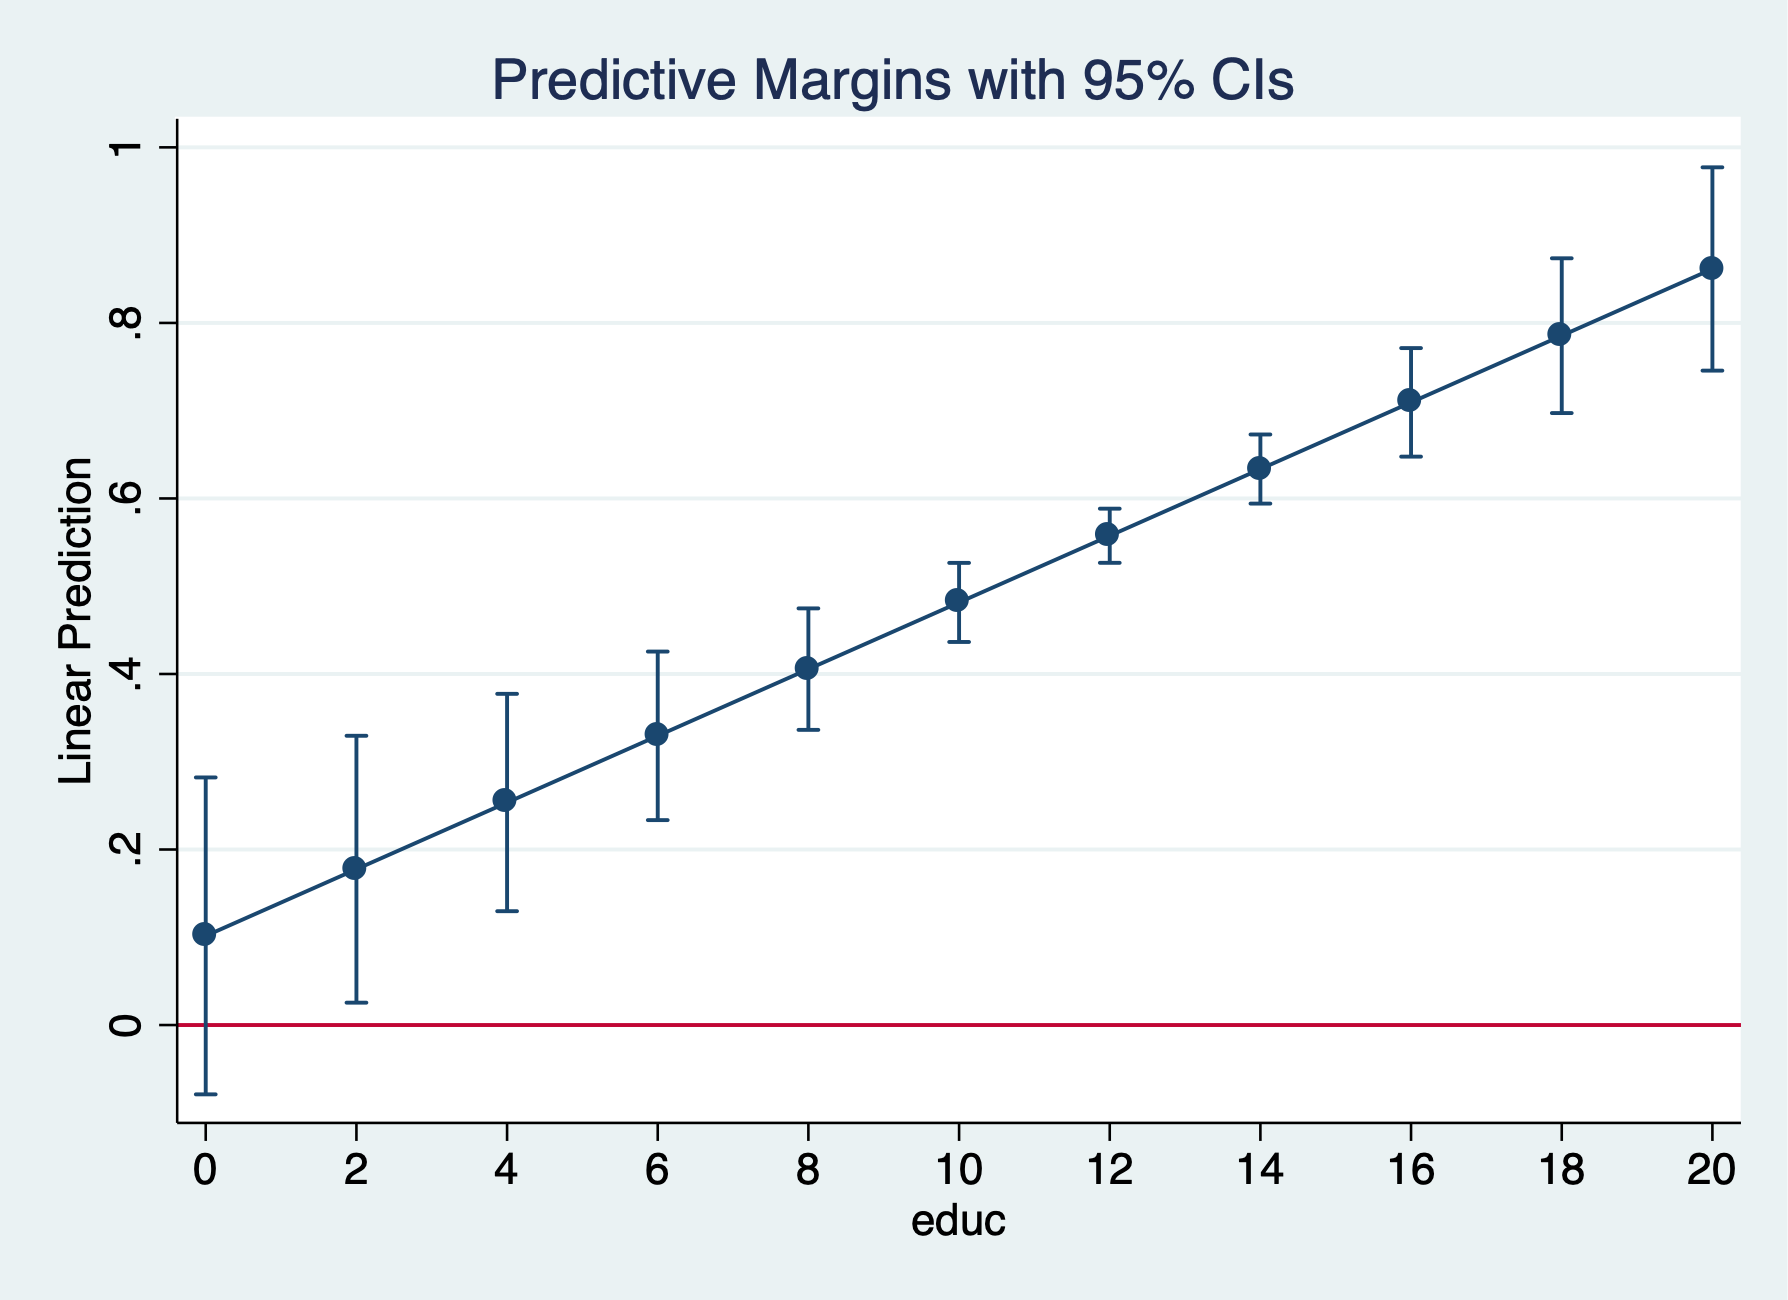
\includegraphics[keepaspectratio]{week8_inlflpm.png}}
\caption{Marginal Effect of Education}
\end{figure}

\subsubsection*{Logit}\label{logit-2}
\addcontentsline{toc}{subsubsection}{Logit}

\begin{Shaded}
\begin{Highlighting}[]
\KeywordTok{quietly} \KeywordTok{logit}\NormalTok{ inlf nwifeinc educ exper expersq kidslt6 kidsge6}
\NormalTok{eststo logit1: margins, }\FunctionTok{at}\NormalTok{(educ=(0(2)20)) }\KeywordTok{post}
\NormalTok{marginsplot, }\KeywordTok{yline}\NormalTok{(0)}
\end{Highlighting}
\end{Shaded}

\begin{figure}
\centering
\pandocbounded{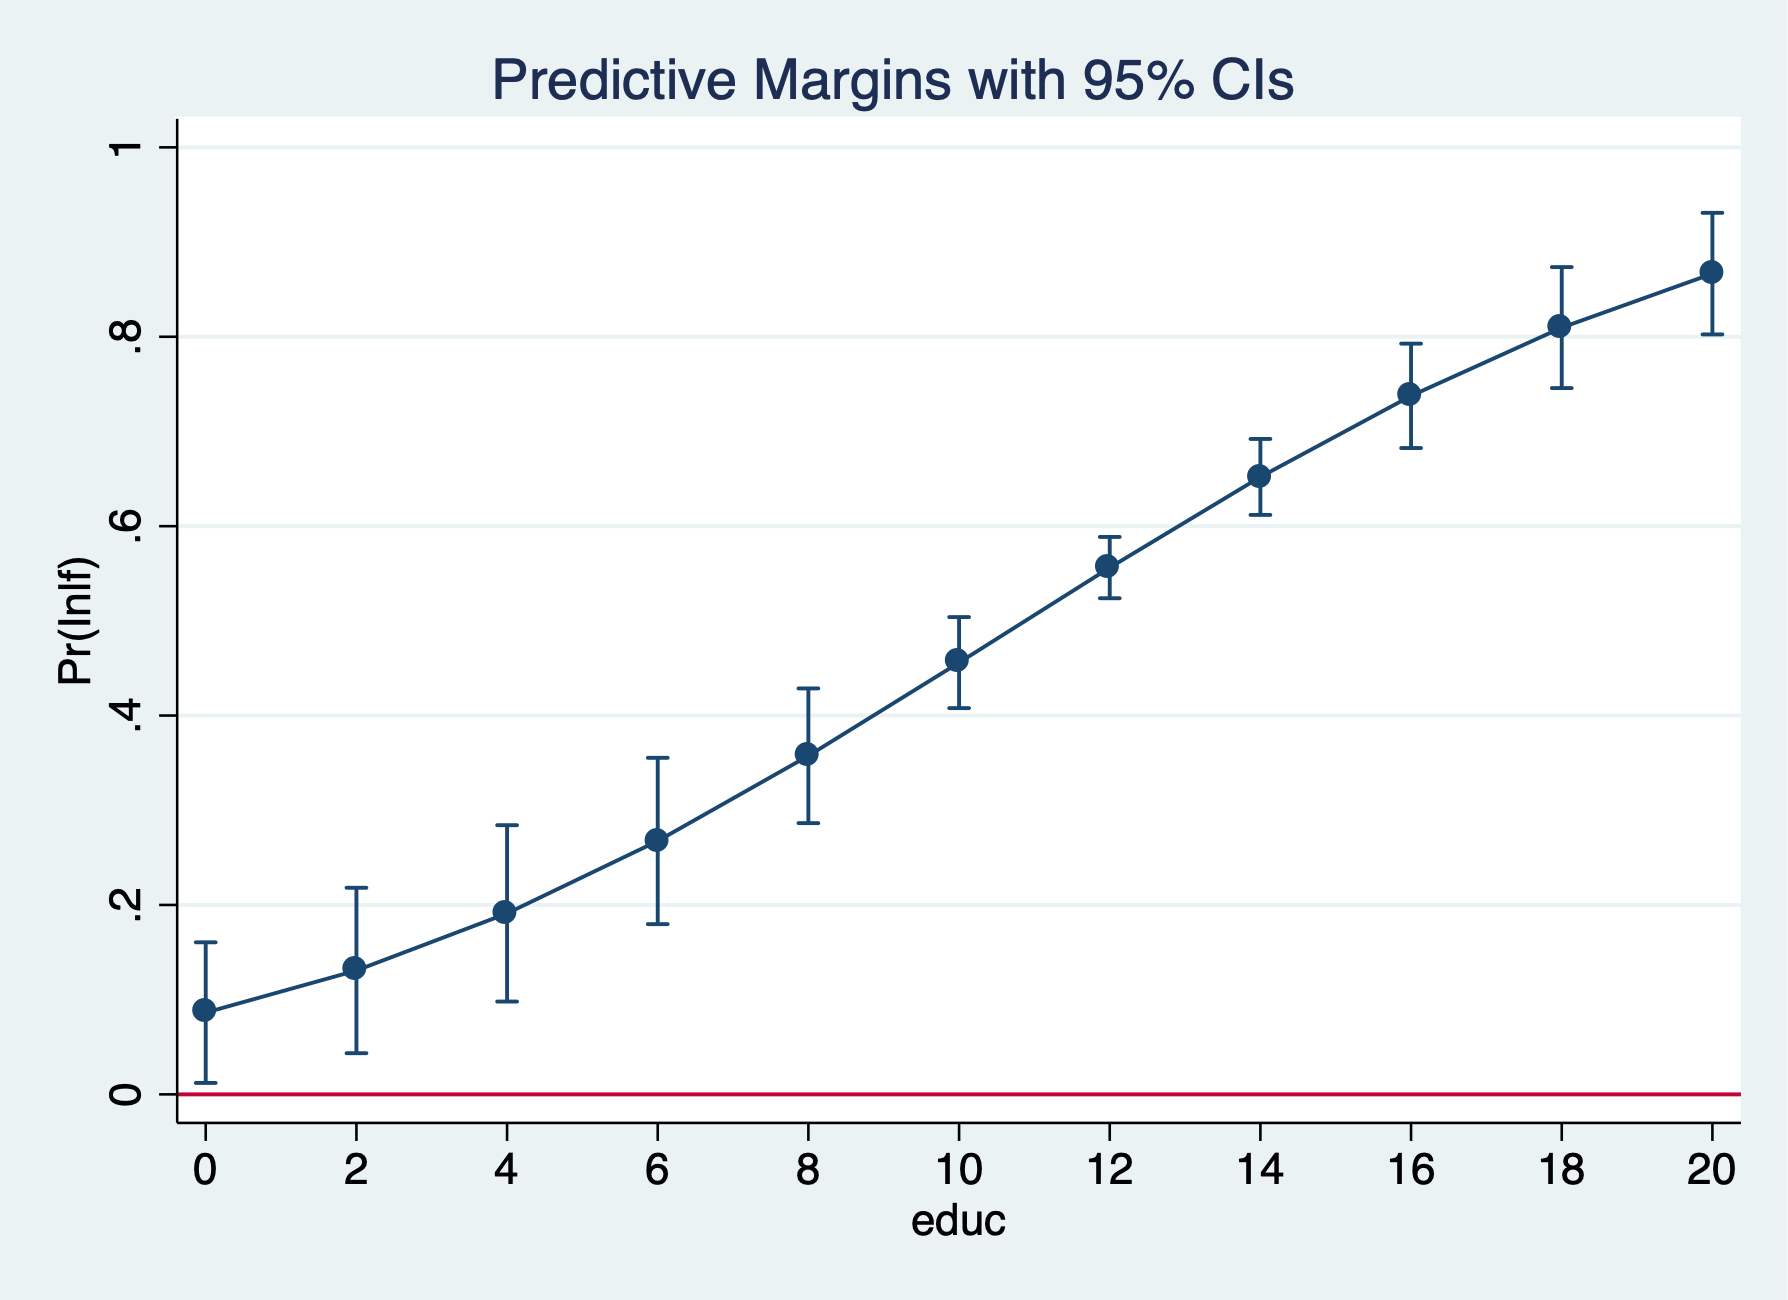
\includegraphics[keepaspectratio]{week8_inlflogit.png}}
\caption{Marginal Effect of Education}
\end{figure}

\subsubsection*{Probit}\label{probit-2}
\addcontentsline{toc}{subsubsection}{Probit}

\begin{Shaded}
\begin{Highlighting}[]
\KeywordTok{quietly} \KeywordTok{probit}\NormalTok{ inlf nwifeinc educ exper expersq age kidslt6 kidsge6}
\NormalTok{eststo probit1: margins, }\FunctionTok{at}\NormalTok{(educ=(0(2)20)) }\KeywordTok{post}
\NormalTok{marginsplot, }\KeywordTok{yline}\NormalTok{(0)}
\end{Highlighting}
\end{Shaded}

The predicted probability that a married women is in the labor force rises from 47.7\% for 12 years of education to 71.2\% for 16 years of education.

\begin{figure}
\centering
\pandocbounded{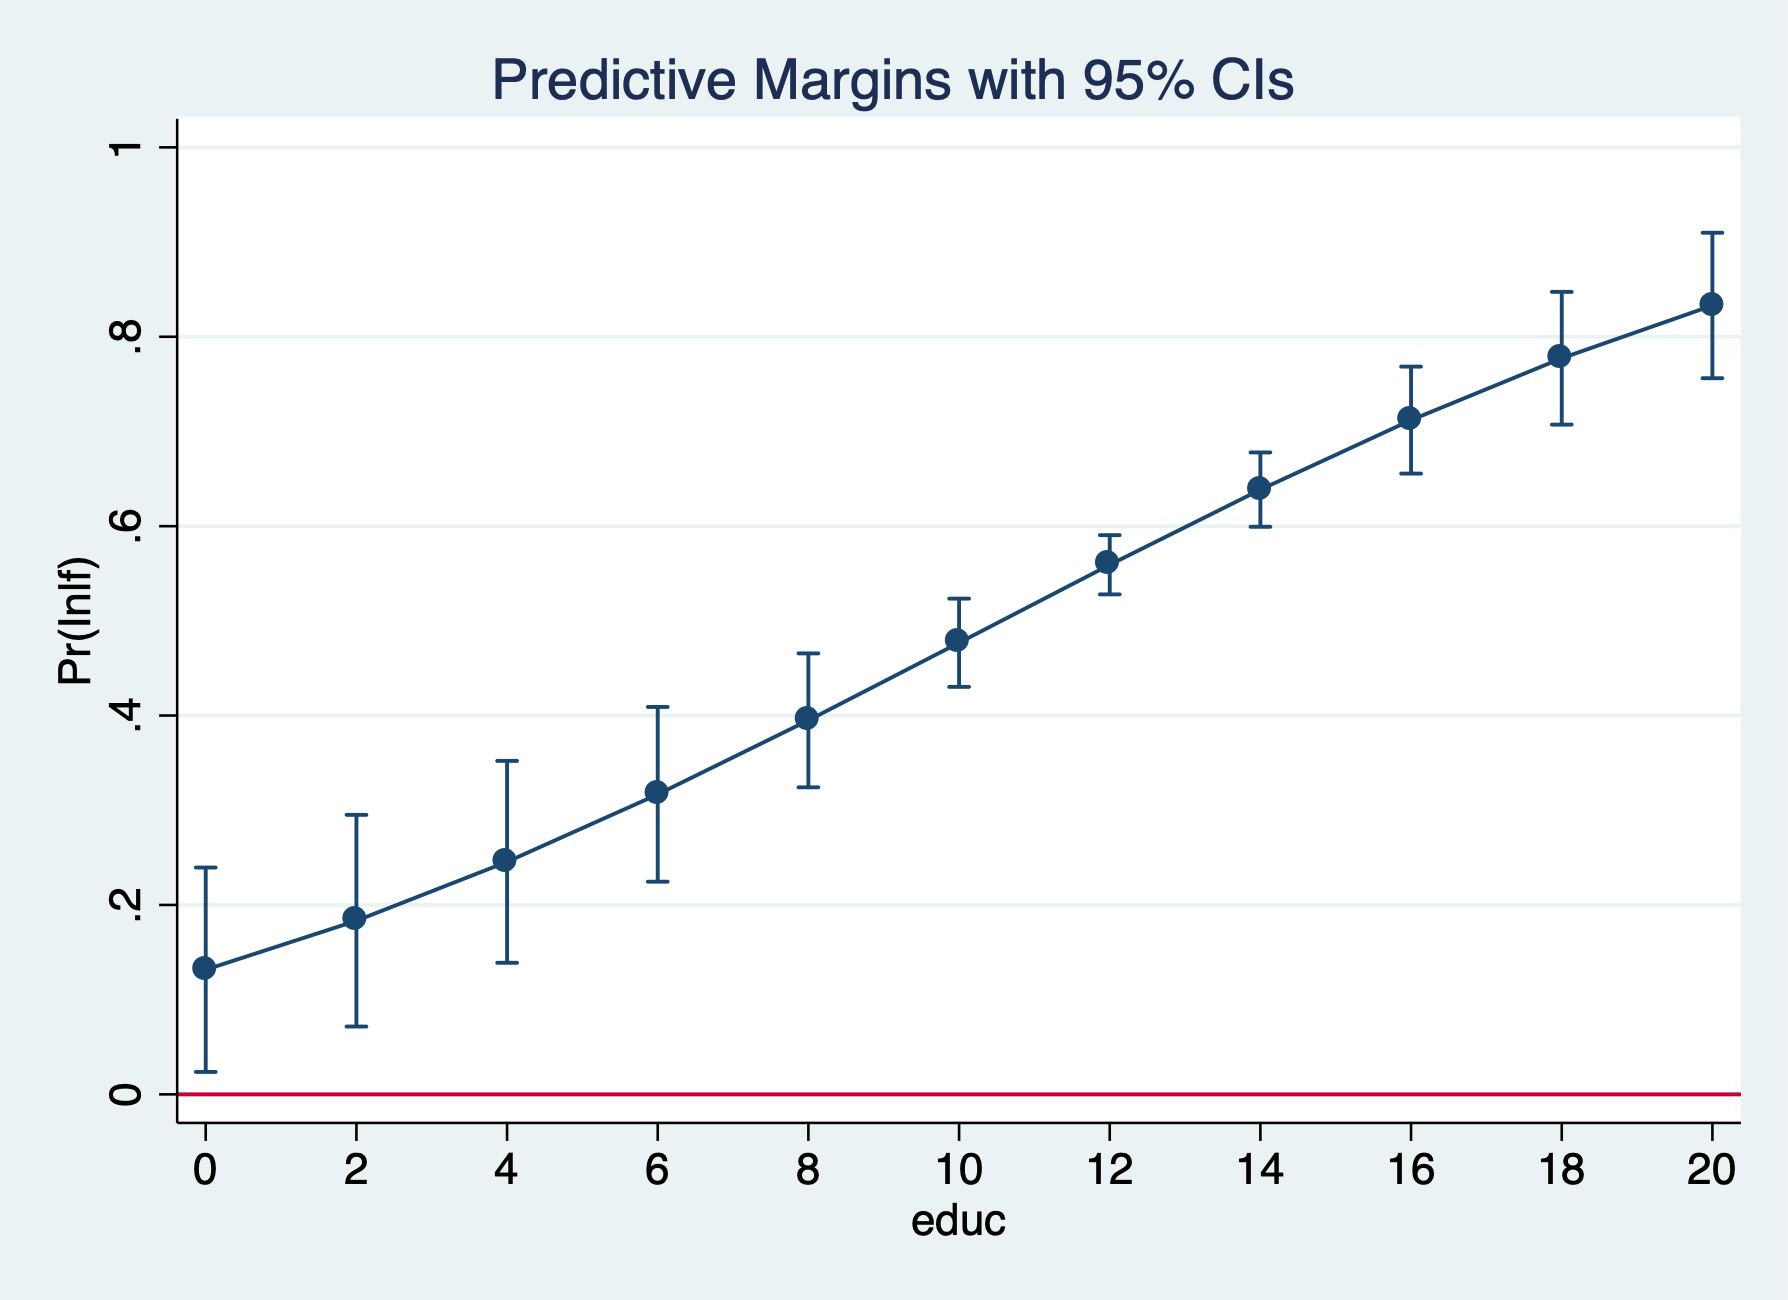
\includegraphics[keepaspectratio]{week8_inlfprobit.png}}
\caption{Marginal Effect of Education}
\end{figure}

\subsubsection*{Coefficient Plot}\label{coefficient-plot}
\addcontentsline{toc}{subsubsection}{Coefficient Plot}

We can also use coefplot to plot our data.

\begin{Shaded}
\begin{Highlighting}[]
\NormalTok{coefplot lpm logit1, }\FunctionTok{at} \KeywordTok{recast}\NormalTok{(}\KeywordTok{line}\NormalTok{) ciopts(}\KeywordTok{recast}\NormalTok{(rline) lpattern(}\KeywordTok{dash}\NormalTok{))}
\NormalTok{coefplot lpm probit1, }\FunctionTok{at} \KeywordTok{recast}\NormalTok{(}\KeywordTok{line}\NormalTok{) ciopts(}\KeywordTok{recast}\NormalTok{(rline) lpattern(}\KeywordTok{dash}\NormalTok{))}
\NormalTok{coefplot logit1 probit1, }\FunctionTok{at} \KeywordTok{recast}\NormalTok{(}\KeywordTok{line}\NormalTok{) ciopts(}\KeywordTok{recast}\NormalTok{(rline) lpattern(}\KeywordTok{dash}\NormalTok{))}
\end{Highlighting}
\end{Shaded}

\subsection*{Marginal Effects of Education at different points along the curve}\label{marginal-effects-of-education-at-different-points-along-the-curve-1}
\addcontentsline{toc}{subsection}{Marginal Effects of Education at different points along the curve}

\subsubsection*{Linear Probability Model (LPM)}\label{linear-probability-model-lpm-3}
\addcontentsline{toc}{subsubsection}{Linear Probability Model (LPM)}

\begin{Shaded}
\begin{Highlighting}[]
\KeywordTok{quietly} \KeywordTok{reg}\NormalTok{ inlf nwifeinc educ exper expersq age kidslt6 kidsge6}
\NormalTok{margins, }\KeywordTok{dydx}\NormalTok{(kidslt6) }\FunctionTok{at}\NormalTok{(educ=(0(2)20))}
\NormalTok{marginsplot, }\KeywordTok{yline}\NormalTok{(0)}
\end{Highlighting}
\end{Shaded}

\subsubsection*{Logit}\label{logit-3}
\addcontentsline{toc}{subsubsection}{Logit}

\begin{Shaded}
\begin{Highlighting}[]
\KeywordTok{quietly} \KeywordTok{logit}\NormalTok{ inlf nwifeinc educ exper expersq kidslt6 kidsge6}
\NormalTok{margins, }\KeywordTok{dydx}\NormalTok{(kidslt6) }\FunctionTok{at}\NormalTok{(educ=(0(2)20))}
\NormalTok{marginsplot, }\KeywordTok{yline}\NormalTok{(0)}
\KeywordTok{graph} \KeywordTok{export} \StringTok{"/Users/Sam/Desktop/Econ 645/Stata/week8\_logitinlf.png"}\NormalTok{, }\KeywordTok{replace}
\end{Highlighting}
\end{Shaded}

\begin{figure}
\centering
\pandocbounded{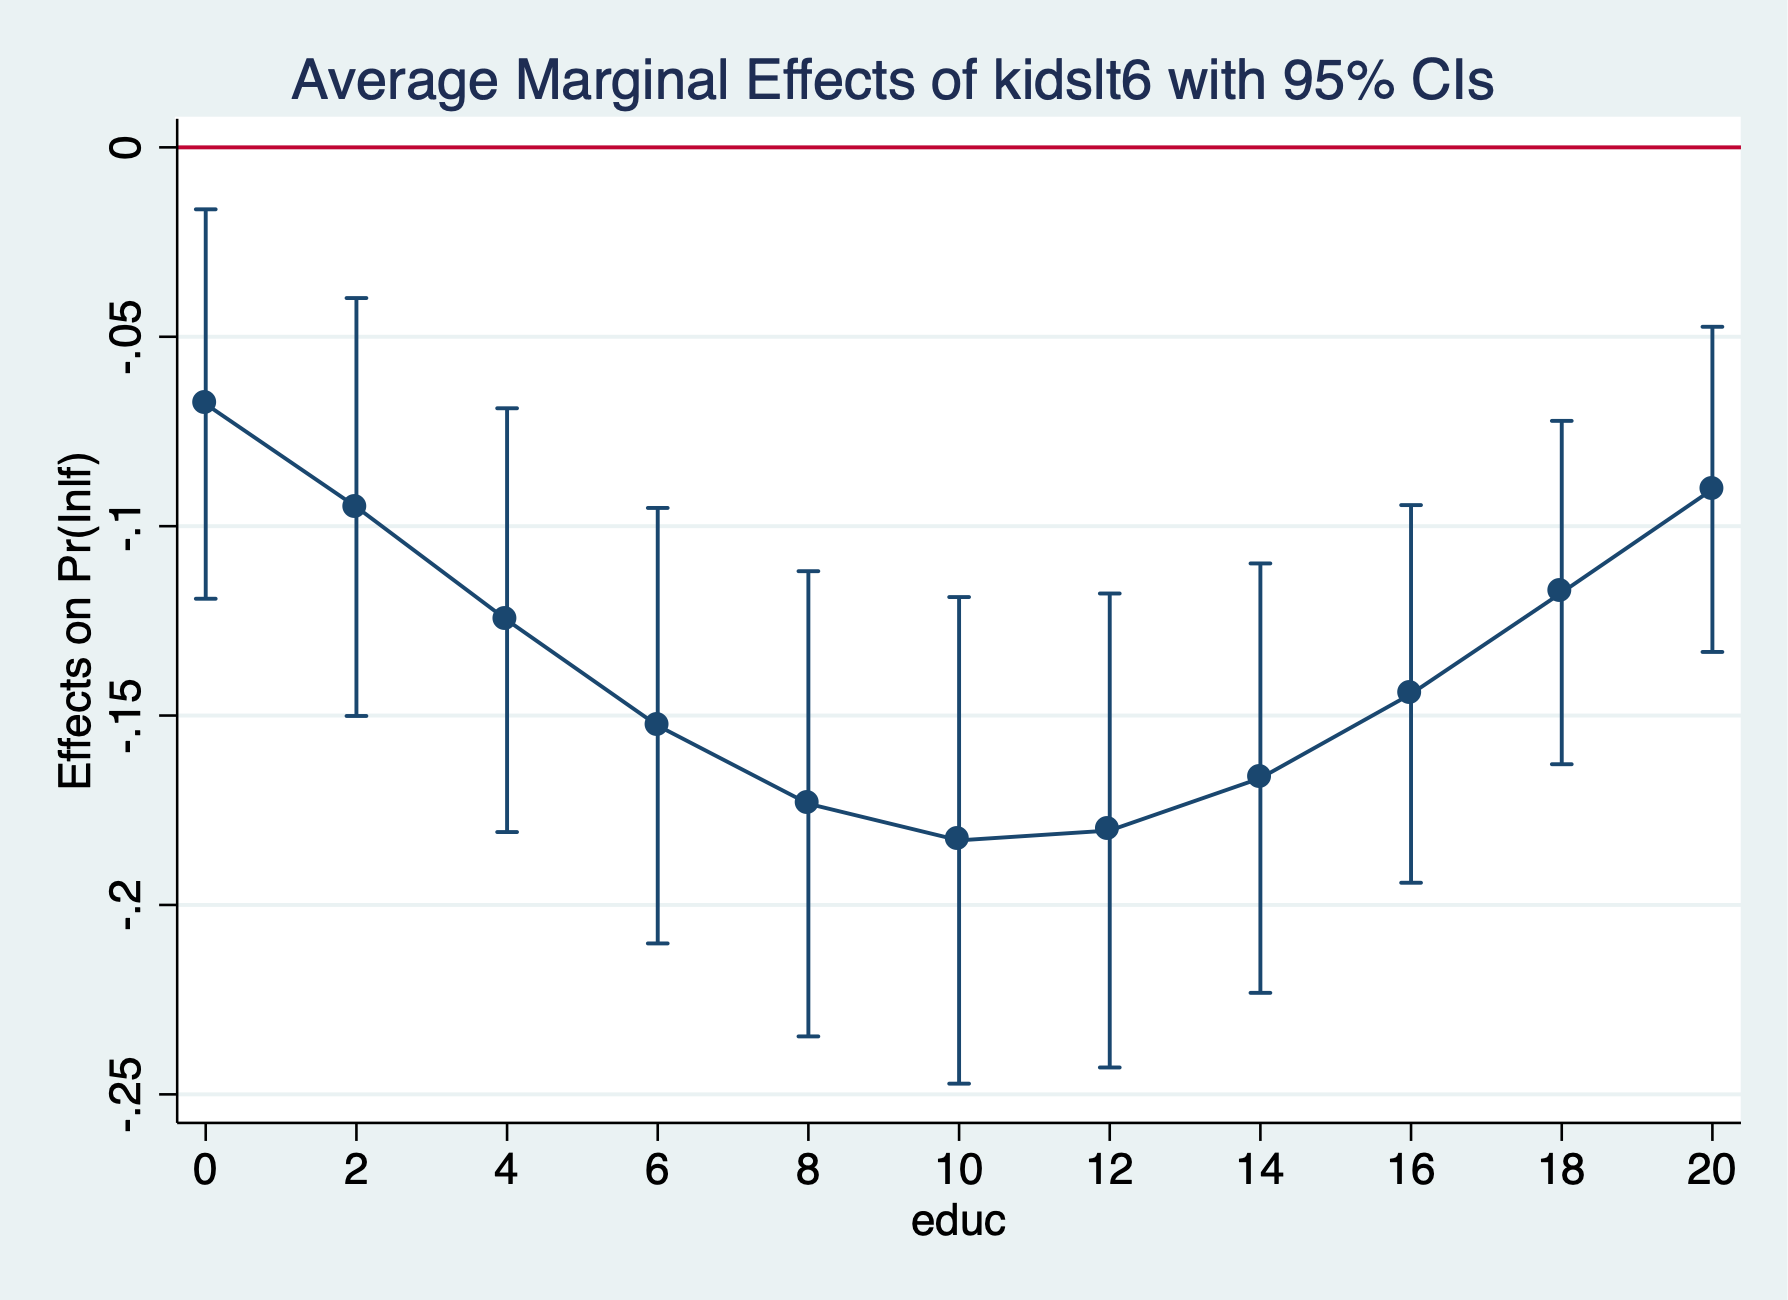
\includegraphics[keepaspectratio]{week8_logitinlf.png}}
\caption{Marginal Effect of Kids Less Than 6}
\end{figure}

\subsubsection*{Probit}\label{probit-3}
\addcontentsline{toc}{subsubsection}{Probit}

\begin{Shaded}
\begin{Highlighting}[]
\KeywordTok{quietly} \KeywordTok{probit}\NormalTok{ inlf nwifeinc educ exper expersq age kidslt6 kidsge6}
\NormalTok{margins, }\KeywordTok{dydx}\NormalTok{(kidslt6) }\FunctionTok{at}\NormalTok{(educ=(0(2)20))}
\NormalTok{marginsplot, }\KeywordTok{yline}\NormalTok{(0)}
\end{Highlighting}
\end{Shaded}

The average marginal effect for an additional child less than 6 rises from -18.3 percentage points to -14.4 percentage points, but the difference does not appear to be statistically significant.

\chapter{Multinominal Logit}\label{multinominal-logit}

Adapted from Long and Freese (2006)

When we have nominal categorical variables, we cannot use a binary logit or probit. We will need to use multinomial logit or probit.

\textbf{Lesson: Interpreting a nominal categorical dependent variable}
We will use Current Population Survey Data from September 2023 and 2024 to estimate the following model for labor force participation:
\[ lfs_{i}=\beta_{0}+\beta_1 edu_{i} + \beta_2 exper_i + ... + u_i \].

There are three alternatives: Employed, Unemployed, and Not in the Labor Force.

\section{Example Current Population Survey}\label{example-current-population-survey}

\begin{Shaded}
\begin{Highlighting}[]
\KeywordTok{use} \StringTok{"/Users/Sam/Desktop/Econ 645/Data/CPS/mlogit\_example.dta"}\NormalTok{, }\KeywordTok{clear}
\KeywordTok{tab}\NormalTok{ laborforce}
\KeywordTok{tab}\NormalTok{ laborforce, }\KeywordTok{nolabel}
\end{Highlighting}
\end{Shaded}

\begin{verbatim}
Labor Force |
     Status |      Freq.     Percent        Cum.
------------+-----------------------------------
   Employed |     23,760       57.12       57.12
 Unemployed |        832        2.00       59.12
       NILF |     17,007       40.88      100.00
------------+-----------------------------------
      Total |     41,599      100.00


Labor Force |
     Status |      Freq.     Percent        Cum.
------------+-----------------------------------
          1 |     23,760       57.12       57.12
          2 |        832        2.00       59.12
          3 |     17,007       40.88      100.00
------------+-----------------------------------
      Total |     41,599      100.00
\end{verbatim}

Our dependent variable has three nominal categories.
\[ y=[1,2,3] \]
оr
\[ y=[Employed, Unemployed, NILF] \]

We use the \emph{mlogit} command to run a multinomial logit to get log odds for \(J-1\) logits.

\begin{Shaded}
\begin{Highlighting}[]
\KeywordTok{mlogit}\NormalTok{ laborforce i.educat }\FunctionTok{exp}\NormalTok{ exp2 i.race\_ethnicity i.female i.metroarea i.}\KeywordTok{union}\NormalTok{ i.marital i.hryear4}
\end{Highlighting}
\end{Shaded}

\begin{verbatim}
Iteration 0:   log likelihood = -31774.039  
Iteration 1:   log likelihood = -22975.759  
Iteration 2:   log likelihood = -22620.368  
Iteration 3:   log likelihood = -22573.244  
Iteration 4:   log likelihood = -22565.789  
Iteration 5:   log likelihood = -22564.343  
Iteration 6:   log likelihood = -22564.014  
Iteration 7:   log likelihood = -22563.941  
Iteration 8:   log likelihood = -22563.925  
Iteration 9:   log likelihood = -22563.922  
Iteration 10:  log likelihood = -22563.922  
Iteration 11:  log likelihood = -22563.922  
Iteration 12:  log likelihood = -22563.922  

Multinomial logistic regression                 Number of obs     =     41,599
                                                LR chi2(38)       =   18420.23
                                                Prob > chi2       =     0.0000
Log likelihood = -22563.922                     Pseudo R2         =     0.2899

-------------------------------------------------------------------------------------------
         laborforcestatus |      Coef.   Std. Err.      z    P>|z|     [95% Conf. Interval]
--------------------------+----------------------------------------------------------------
Employed                  |  (base outcome)
--------------------------+----------------------------------------------------------------
Unemployed                |
                   educat |
                     HSD  |  -.2279524   .1119685    -2.04   0.042    -.4474066   -.0084982
            Some College  |  -.4312492   .1303621    -3.31   0.001    -.6867542   -.1757442
           AA/Vocational  |  -.6931682    .165487    -4.19   0.000    -1.017517   -.3688197
                   BS/BA  |  -.6706784   .1331892    -5.04   0.000    -.9317245   -.4096323
Graduate or Professional  |  -1.063383   .1745188    -6.09   0.000    -1.405433   -.7213323
                          |
                      exp |  -.0291051   .0088759    -3.28   0.001    -.0465016   -.0117087
                     exp2 |   .0002524   .0001575     1.60   0.109    -.0000562    .0005611
                          |
           race_ethnicity |
  Asian/Pacific Islander  |   -.813795   .3012644    -2.70   0.007    -1.404262   -.2233275
                   Black  |  -.3951124   .2756281    -1.43   0.152    -.9353337    .1451088
         Hispanic/Latino  |  -.6504449   .2691511    -2.42   0.016    -1.177971   -.1229184
                   White  |  -.7855686   .2616547    -3.00   0.003    -1.298402   -.2727347
             Multiracial  |  -.4798449   .3366208    -1.43   0.154     -1.13961    .1799197
                          |
                   female |
                  Female  |  -.0004137   .0721979    -0.01   0.995     -.141919    .1410915
                          |
                metroarea |
           Nonmetro Area  |  -.1010417    .097797    -1.03   0.302    -.2927204    .0906369
          Not Identified  |   .0635435    .346152     0.18   0.854     -.614902     .741989
                          |
                    union |
                   Union  |  -19.66515   2339.277    -0.01   0.993    -4604.564    4565.234
                          |
                  marital |
    Divorced/Sep/Widowed  |   .6132556   .1175463     5.22   0.000     .3828691     .843642
           Never Married  |   .7526873   .0988405     7.62   0.000     .5589634    .9464112
                          |
                  hryear4 |
                    2024  |   .0228376    .071126     0.32   0.748    -.1165667    .1622419
                          |
                    _cons |  -2.023219   .3012462    -6.72   0.000    -2.613651   -1.432787
--------------------------+----------------------------------------------------------------
NILF                      |
                   educat |
                     HSD  |  -.7898216   .0425444   -18.56   0.000    -.8732071   -.7064361
            Some College  |  -.8941042   .0479568   -18.64   0.000    -.9880978   -.8001105
           AA/Vocational  |  -1.143176   .0559087   -20.45   0.000    -1.252755   -1.033597
                   BS/BA  |  -1.493236   .0488335   -30.58   0.000    -1.588948   -1.397524
Graduate or Professional  |  -1.746904   .0561914   -31.09   0.000    -1.857038   -1.636771
                          |
                      exp |  -.1490983    .003087   -48.30   0.000    -.1551487    -.143048
                     exp2 |   .0031412   .0000469    66.92   0.000     .0030492    .0032332
                          |
           race_ethnicity |
  Asian/Pacific Islander  |  -.1995846   .1336975    -1.49   0.135    -.4616269    .0624578
                   Black  |  -.1053158   .1293382    -0.81   0.415     -.358814    .1481824
         Hispanic/Latino  |  -.4785722   .1270357    -3.77   0.000    -.7275575   -.2295869
                   White  |  -.3378929   .1237786    -2.73   0.006    -.5804944   -.0952913
             Multiracial  |  -.1802636   .1537778    -1.17   0.241    -.4816625    .1211354
                          |
                   female |
                  Female  |   .5781835   .0258942    22.33   0.000     .5274318    .6289351
                          |
                metroarea |
           Nonmetro Area  |  -.0069684   .0328081    -0.21   0.832    -.0712712    .0573344
          Not Identified  |  -.0021328   .1282129    -0.02   0.987    -.2534254    .2491598
                          |
                    union |
                   Union  |  -20.25621   566.9973    -0.04   0.972     -1131.55    1091.038
                          |
                  marital |
    Divorced/Sep/Widowed  |  -.0531382   .0373157    -1.42   0.154    -.1262757    .0199993
           Never Married  |   .1464745   .0379587     3.86   0.000     .0720769    .2208722
                          |
                  hryear4 |
                    2024  |  -.0398405   .0253899    -1.57   0.117    -.0896037    .0099228
                          |
                    _cons |   1.072448   .1365064     7.86   0.000     .8049003    1.339996
-------------------------------------------------------------------------------------------
Note: 2044 observations completely determined.  Standard errors questionable.
\end{verbatim}

These are log-odds coefficients comparing the coefficients for unemployed and not in the labor force to employed. Let's use odds ratios.

\subsection{Relative Risk Ratios}\label{relative-risk-ratios}

Akin to our odds ratios, relative risk ratios are \[ e^{\beta_j} \]

\begin{Shaded}
\begin{Highlighting}[]
\KeywordTok{mlogit}\NormalTok{ laborforce i.educat }\FunctionTok{exp}\NormalTok{ exp2 i.race\_ethnicity i.female i.metroarea i.}\KeywordTok{union}\NormalTok{ i.marital i.hryear4, rrr}
\end{Highlighting}
\end{Shaded}

\begin{verbatim}
Iteration 0:   log likelihood = -31774.039  
Iteration 1:   log likelihood = -22975.759  
Iteration 2:   log likelihood = -22620.368  
Iteration 3:   log likelihood = -22573.244  
Iteration 4:   log likelihood = -22565.789  
Iteration 5:   log likelihood = -22564.343  
Iteration 6:   log likelihood = -22564.014  
Iteration 7:   log likelihood = -22563.941  
Iteration 8:   log likelihood = -22563.925  
Iteration 9:   log likelihood = -22563.922  
Iteration 10:  log likelihood = -22563.922  
Iteration 11:  log likelihood = -22563.922  
Iteration 12:  log likelihood = -22563.922  

Multinomial logistic regression                 Number of obs     =     41,599
                                                LR chi2(38)       =   18420.23
                                                Prob > chi2       =     0.0000
Log likelihood = -22563.922                     Pseudo R2         =     0.2899

-------------------------------------------------------------------------------------------
         laborforcestatus |        RRR   Std. Err.      z    P>|z|     [95% Conf. Interval]
--------------------------+----------------------------------------------------------------
Employed                  |  (base outcome)
--------------------------+----------------------------------------------------------------
Unemployed                |
                   educat |
                     HSD  |   .7961621   .0891451    -2.04   0.042     .6392839    .9915378
            Some College  |    .649697   .0846959    -3.31   0.001     .5032067    .8388326
           AA/Vocational  |   .4999895   .0827417    -4.19   0.000     .3614915    .6915501
                   BS/BA  |   .5113616   .0681079    -5.04   0.000     .3938739    .6638943
Graduate or Professional  |   .3452858   .0602589    -6.09   0.000     .2452608    .4861042
                          |
                      exp |   .9713143   .0086213    -3.28   0.001      .954563    .9883596
                     exp2 |   1.000252   .0001575     1.60   0.109     .9999438    1.000561
                          |
           race_ethnicity |
  Asian/Pacific Islander  |    .443173   .1335123    -2.70   0.007     .2455481    .7998528
                   Black  |   .6736043   .1856643    -1.43   0.152     .3924549    1.156165
         Hispanic/Latino  |   .5218136   .1404467    -2.42   0.016     .3079027    .8843359
                   White  |   .4558604    .119278    -3.00   0.003     .2729675    .7612947
             Multiracial  |   .6188793   .2083277    -1.43   0.154     .3199439    1.197121
                          |
                   female |
                  Female  |   .9995863    .072168    -0.01   0.995     .8676915     1.15153
                          |
                metroarea |
           Nonmetro Area  |   .9038953   .0883983    -1.03   0.302     .7462308    1.094871
          Not Identified  |   1.065606   .3688616     0.18   0.854     .5406939    2.100108
                          |
                    union |
                   Union  |   2.88e-09   6.74e-06    -0.01   0.993            0           .
                          |
                  marital |
    Divorced/Sep/Widowed  |   1.846433   .2170413     5.22   0.000     1.466486    2.324819
           Never Married  |   2.122697   .2098085     7.62   0.000     1.748859    2.576447
                          |
                  hryear4 |
                    2024  |     1.0231    .072769     0.32   0.748     .8899707    1.176145
                          |
                    _cons |   .1322292   .0398335    -6.72   0.000     .0732666    .2386429
--------------------------+----------------------------------------------------------------
NILF                      |
                   educat |
                     HSD  |   .4539258    .019312   -18.56   0.000     .4176101    .4933995
            Some College  |   .4089738   .0196131   -18.64   0.000     .3722842    .4492793
           AA/Vocational  |   .3188048    .017824   -20.45   0.000     .2857165     .355725
                   BS/BA  |   .2246446   .0109702   -30.58   0.000     .2041403    .2472084
Graduate or Professional  |   .1743127   .0097949   -31.09   0.000     .1561345    .1946073
                          |
                      exp |   .8614844   .0026594   -48.30   0.000     .8562879    .8667124
                     exp2 |   1.003146   .0000471    66.92   0.000     1.003054    1.003238
                          |
           race_ethnicity |
  Asian/Pacific Islander  |   .8190709   .1095078    -1.49   0.135     .6302574     1.06445
                   Black  |   .9000402   .1164096    -0.81   0.415     .6985043    1.159724
         Hispanic/Latino  |   .6196675   .0787199    -3.77   0.000     .4830875    .7948619
                   White  |   .7132717   .0882878    -2.73   0.006     .5596216     .909108
             Multiracial  |   .8350501   .1284122    -1.17   0.241     .6177555    1.128778
                          |
                   female |
                  Female  |   1.782797    .046164    22.33   0.000     1.694575    1.875612
                          |
                metroarea |
           Nonmetro Area  |   .9930558   .0325803    -0.21   0.832     .9312093     1.05901
          Not Identified  |   .9978694   .1279397    -0.02   0.987     .7761376    1.282947
                          |
                    union |
                   Union  |   1.60e-09   9.05e-07    -0.04   0.972            0           .
                          |
                  marital |
    Divorced/Sep/Widowed  |    .948249   .0353846    -1.42   0.154     .8813718    1.020201
           Never Married  |   1.157745   .0439465     3.86   0.000     1.074738    1.247164
                          |
                  hryear4 |
                    2024  |   .9609427   .0243982    -1.57   0.117     .9142935    1.009972
                          |
                    _cons |   2.922525   .3989434     7.86   0.000     2.236473    3.819027
-------------------------------------------------------------------------------------------
Note: 2044 observations completely determined.  Standard errors questionable.
\end{verbatim}

\subsubsection{Unemployed relative to employed}\label{unemployed-relative-to-employed}

For an individual with a high school degree relative to a high school drop out, the relative risk for being unemployed relative to employed decreases by a factor of 0.80

For an individual with some college relative to a high school drop out, the relative risk for being unemployed relative to employed decreases by a factor of 0.65

For an individual with an AA or vocational degree relative to a high school drop out, the relative risk for being unemployed relative to employed decreases by a factor of 0.50

For an individual with a BS/BA degree relative to a high school drop out, the relative risk for being unemployed relative to employed decreases by a factor of 0.51

For an individual with a graduate or professional degree relative to a high school drop out, the relative risk for being unemployed relative to employed decreases by a factor of 0.35

\subsubsection{Not in the labor force relative to employed}\label{not-in-the-labor-force-relative-to-employed}

For an individual with a high school degree relative to a high school drop out, the relative risk for being NILF relative to employed decreases by a factor of 0.45

For an individual with some college relative to a high school drop out, the relative risk for being NILF relative to employed decreases by a factor of 0.41

For an individual with an AA or vocational degree relative to a high school drop out, the relative risk for being NILF relative to employed decreases by a factor of 0.32

For an individual with a BS/BA degree relative to a high school drop out, the relative risk for being NILF relative to employed decreases by a factor of 0.22

For an individual with a graduate or professional degree relative to a high school drop out, the relative risk for being NILF relative to employed decreases by a factor of 0.17

\section{Test for Independence of Irrelevant Alternative Assumption}\label{test-for-independence-of-irrelevant-alternative-assumption}

Next, we need to test our Independence of Irrelevant Alternatives (IIA) assumption with a Hausman Test.

\subsection{Estimate an Unrestricted model - We'll remove unemployed}\label{estimate-an-unrestricted-model---well-remove-unemployed}

\begin{Shaded}
\begin{Highlighting}[]
\KeywordTok{quietly} \KeywordTok{mlogit}\NormalTok{ laborforce i.educat }\FunctionTok{exp}\NormalTok{ exp2 i.race\_ethnicity i.female i.metroarea i.}\KeywordTok{union}\NormalTok{ i.marital i.hryear4}
\KeywordTok{estimates} \KeywordTok{store}\NormalTok{ unrestricted}
\end{Highlighting}
\end{Shaded}

We compare the log odds for unemployed and not in the labor force to being employed. Given that these are log odds, we'll need to convert them to Odds Ratios or find the marginal effects.

\subsection{Estimate a Restricted Model to test Independence of Irrelevant Alternatives assumption}\label{estimate-a-restricted-model-to-test-independence-of-irrelevant-alternatives-assumption}

\begin{Shaded}
\begin{Highlighting}[]
\KeywordTok{quietly} \KeywordTok{mlogit}\NormalTok{ laborforce i.educat }\FunctionTok{exp}\NormalTok{ exp2 i.race\_ethnicity i.female i.metroarea i.}\KeywordTok{union}\NormalTok{ i.marital }\KeywordTok{if}\NormalTok{ laborforce !=2}
\NormalTok{estimate }\KeywordTok{store}\NormalTok{ restricted}
\end{Highlighting}
\end{Shaded}

\subsection{Use hausman command}\label{use-hausman-command}

\begin{Shaded}
\begin{Highlighting}[]
\KeywordTok{hausman}\NormalTok{ restricted unrestricted, alleqs constant}
\end{Highlighting}
\end{Shaded}

\begin{verbatim}
Note: the rank of the differenced variance matrix (2) does not equal the number of coefficients being tested (19); be
        sure this is what you expect, or there may be problems computing the test.  Examine the output of your
        estimators for anything unexpected and possibly consider scaling your variables so that the coefficients are
        on a similar scale.

                 ---- Coefficients ----
             |      (b)          (B)            (b-B)     sqrt(diag(V_b-V_B))
             |   restricted  unrestricted    Difference          S.E.
-------------+----------------------------------------------------------------
      educat |
          2  |   -.7860864    -.7898216        .0037352        .0035785
          3  |     -.89149    -.8941042        .0026142        .0032032
          4  |   -1.140012    -1.143176         .003164         .003669
          5  |   -1.486705    -1.493236        .0065306        .0036976
          6  |   -1.737118    -1.746904        .0097867        .0035815
         exp |   -.1486206    -.1490983        .0004777        .0002218
        exp2 |    .0031335     .0031412       -7.78e-06        2.91e-06
race_ethni~y |
          2  |   -.1712505    -.1995846        .0283341        .0120289
          3  |   -.0717454    -.1053158        .0335704        .0121412
          4  |   -.4427331    -.4785722        .0358391        .0115676
          5  |   -.3060009    -.3378929         .031892        .0117006
          6  |   -.1491388    -.1802636        .0311247        .0136923
    1.female |    .5793374     .5781835        .0011539        .0018992
   metroarea |
          2  |   -.0070074    -.0069684        -.000039         .002025
          3  |   -.0064057    -.0021328       -.0042729        .0112617
     1.union |   -20.20846    -20.25621        .0477553               .
     marital |
          2  |   -.0524486    -.0531382        .0006896        .0022895
          3  |    .1495841     .1464745        .0031096        .0023193
       _cons |     1.00979     1.072448       -.0626578               .
------------------------------------------------------------------------------
                          b = consistent under Ho and Ha; obtained from mlogit
           B = inconsistent under Ha, efficient under Ho; obtained from mlogit

    Test:  Ho:  difference in coefficients not systematic

                  chi2(2) = (b-B)'[(V_b-V_B)^(-1)](b-B)
                          =        8.92
                Prob>chi2 =      0.0116
                (V_b-V_B is not positive definite)
\end{verbatim}

Our chi-squared is 8.92, which means with reject the IIA assumption. We should consider a binary response here.

\subsection{Predicted Probabilities}\label{predicted-probabilities}

Next, we use Stata to estimate predicted probabilities

\begin{Shaded}
\begin{Highlighting}[]
\KeywordTok{quietly} \KeywordTok{mlogit}\NormalTok{ laborforce i.educat }\FunctionTok{exp}\NormalTok{ exp2 i.race\_ethnicity i.female i.metroarea i.}\KeywordTok{union}\NormalTok{ i.marital, base(1)}
\NormalTok{margins, atmeans }\KeywordTok{predict}\NormalTok{(outcome(1))}
\NormalTok{margins, atmeans }\KeywordTok{predict}\NormalTok{(outcome(2))}
\NormalTok{margins, atmeans }\KeywordTok{predict}\NormalTok{(outcome(3))}
\end{Highlighting}
\end{Shaded}

\begin{verbatim}
Adjusted predictions                            Number of obs     =     41,599
Model VCE    : OIM

Expression   : Pr(laborforcestatus==Employed), predict(outcome(1))
at           : 1.educat        =    .1261088 (mean)
               2.educat        =     .286954 (mean)
               3.educat        =    .1488497 (mean)
               4.educat        =    .0969254 (mean)
               5.educat        =    .2079617 (mean)
               6.educat        =    .1332003 (mean)
               exp             =    32.89247 (mean)
               exp2            =    1467.595 (mean)
               1.race_eth~y    =    .0098079 (mean)
               2.race_eth~y    =    .0622611 (mean)
               3.race_eth~y    =    .0931032 (mean)
               4.race_eth~y    =    .1487776 (mean)
               5.race_eth~y    =    .6685738 (mean)
               6.race_eth~y    =    .0174764 (mean)
               0.female        =    .4804923 (mean)
               1.female        =    .5195077 (mean)
               1.metroarea     =    .8000673 (mean)
               2.metroarea     =    .1904132 (mean)
               3.metroarea     =    .0095195 (mean)
               0.union         =    .9508642 (mean)
               1.union         =    .0491358 (mean)
               1.marital       =    .5163586 (mean)
               2.marital       =    .1819515 (mean)
               3.marital       =    .3016899 (mean)

------------------------------------------------------------------------------
             |            Delta-method
             |     Margin   Std. Err.      z    P>|z|     [95% Conf. Interval]
-------------+----------------------------------------------------------------
       _cons |   .7684672   4.830264     0.16   0.874    -8.698677    10.23561
------------------------------------------------------------------------------


Adjusted predictions                            Number of obs     =     41,599
Model VCE    : OIM

Expression   : Pr(laborforcestatus==Unemployed), predict(outcome(2))
at           : 1.educat        =    .1261088 (mean)
               2.educat        =     .286954 (mean)
               3.educat        =    .1488497 (mean)
               4.educat        =    .0969254 (mean)
               5.educat        =    .2079617 (mean)
               6.educat        =    .1332003 (mean)
               exp             =    32.89247 (mean)
               exp2            =    1467.595 (mean)
               1.race_eth~y    =    .0098079 (mean)
               2.race_eth~y    =    .0622611 (mean)
               3.race_eth~y    =    .0931032 (mean)
               4.race_eth~y    =    .1487776 (mean)
               5.race_eth~y    =    .6685738 (mean)
               6.race_eth~y    =    .0174764 (mean)
               0.female        =    .4804923 (mean)
               1.female        =    .5195077 (mean)
               1.metroarea     =    .8000673 (mean)
               2.metroarea     =    .1904132 (mean)
               3.metroarea     =    .0095195 (mean)
               0.union         =    .9508642 (mean)
               1.union         =    .0491358 (mean)
               1.marital       =    .5163586 (mean)
               2.marital       =    .1819515 (mean)
               3.marital       =    .3016899 (mean)

------------------------------------------------------------------------------
             |            Delta-method
             |     Margin   Std. Err.      z    P>|z|     [95% Conf. Interval]
-------------+----------------------------------------------------------------
       _cons |   .0090578    1.03352     0.01   0.993    -2.016605     2.03472
------------------------------------------------------------------------------


Adjusted predictions                            Number of obs     =     41,599
Model VCE    : OIM

Expression   : Pr(laborforcestatus==NILF), predict(outcome(3))
at           : 1.educat        =    .1261088 (mean)
               2.educat        =     .286954 (mean)
               3.educat        =    .1488497 (mean)
               4.educat        =    .0969254 (mean)
               5.educat        =    .2079617 (mean)
               6.educat        =    .1332003 (mean)
               exp             =    32.89247 (mean)
               exp2            =    1467.595 (mean)
               1.race_eth~y    =    .0098079 (mean)
               2.race_eth~y    =    .0622611 (mean)
               3.race_eth~y    =    .0931032 (mean)
               4.race_eth~y    =    .1487776 (mean)
               5.race_eth~y    =    .6685738 (mean)
               6.race_eth~y    =    .0174764 (mean)
               0.female        =    .4804923 (mean)
               1.female        =    .5195077 (mean)
               1.metroarea     =    .8000673 (mean)
               2.metroarea     =    .1904132 (mean)
               3.metroarea     =    .0095195 (mean)
               0.union         =    .9508642 (mean)
               1.union         =    .0491358 (mean)
               1.marital       =    .5163586 (mean)
               2.marital       =    .1819515 (mean)
               3.marital       =    .3016899 (mean)

------------------------------------------------------------------------------
             |            Delta-method
             |     Margin   Std. Err.      z    P>|z|     [95% Conf. Interval]
-------------+----------------------------------------------------------------
       _cons |   .2224751   4.825216     0.05   0.963    -9.234774    9.679725
------------------------------------------------------------------------------
\end{verbatim}

\subsection{Average Marginal Effects}\label{average-marginal-effects}

\begin{Shaded}
\begin{Highlighting}[]
\NormalTok{margins, }\KeywordTok{dydx}\NormalTok{(*) }\KeywordTok{predict}\NormalTok{(outcome(1))}
\NormalTok{margins, }\KeywordTok{dydx}\NormalTok{(*) }\KeywordTok{predict}\NormalTok{(outcome(2))}
\NormalTok{margins, }\KeywordTok{dydx}\NormalTok{(*) }\KeywordTok{predict}\NormalTok{(outcome(3))}
\end{Highlighting}
\end{Shaded}

\begin{verbatim}
Average marginal effects                        Number of obs     =     41,599
Model VCE    : OIM

Expression   : Pr(laborforcestatus==Employed), predict(outcome(1))
dy/dx w.r.t. : 2.educat 3.educat 4.educat 5.educat 6.educat exp exp2 2.race_ethnicity 3.race_ethnicity
               4.race_ethnicity 5.race_ethnicity 6.race_ethnicity 1.female 2.metroarea 3.metroarea 1.union 2.marital
               3.marital

-------------------------------------------------------------------------------------------
                          |            Delta-method
                          |      dy/dx   Std. Err.      z    P>|z|     [95% Conf. Interval]
--------------------------+----------------------------------------------------------------
                   educat |
                     HSD  |   .1309012   .0072675    18.01   0.000     .1166572    .1451452
            Some College  |   .1499942   .0080928    18.53   0.000     .1341326    .1658558
           AA/Vocational  |   .1911979   .0091537    20.89   0.000     .1732569    .2091389
                   BS/BA  |   .2407492   .0078942    30.50   0.000     .2252768    .2562215
Graduate or Professional  |   .2789487    .008527    32.71   0.000     .2622362    .2956613
                          |
                      exp |   .0219808   .0004288    51.26   0.000     .0211403    .0228213
                     exp2 |  -.0004585   5.91e-06   -77.62   0.000      -.00047   -.0004469
                          |
           race_ethnicity |
  Asian/Pacific Islander  |   .0417403   .0212777     1.96   0.050     .0000368    .0834438
                   Black  |   .0224391   .0206352     1.09   0.277    -.0180052    .0628834
         Hispanic/Latino  |   .0802357   .0202145     3.97   0.000     .0406159    .1198555
                   White  |   .0618266   .0197636     3.13   0.002     .0230907    .1005625
             Multiracial  |   .0348149    .024377     1.43   0.153    -.0129632     .082593
                          |
                   female |
                  Female  |  -.0839096   .0039186   -21.41   0.000    -.0915899   -.0762292
                          |
                metroarea |
           Nonmetro Area  |   .0022776   .0050425     0.45   0.652    -.0076056    .0121607
          Not Identified  |  -.0007629   .0197304    -0.04   0.969    -.0394337    .0379079
                          |
                    union |
                   Union  |   .4414329   .0020464   215.71   0.000     .4374219    .4454438
                          |
                  marital |
    Divorced/Sep/Widowed  |   .0001626   .0057357     0.03   0.977    -.0110791    .0114043
           Never Married  |   -.030733    .005813    -5.29   0.000    -.0421263   -.0193397
-------------------------------------------------------------------------------------------
Note: dy/dx for factor levels is the discrete change from the base level.


Average marginal effects                        Number of obs     =     41,599
Model VCE    : OIM

Expression   : Pr(laborforcestatus==Unemployed), predict(outcome(2))
dy/dx w.r.t. : 2.educat 3.educat 4.educat 5.educat 6.educat exp exp2 2.race_ethnicity 3.race_ethnicity
               4.race_ethnicity 5.race_ethnicity 6.race_ethnicity 1.female 2.metroarea 3.metroarea 1.union 2.marital
               3.marital

-------------------------------------------------------------------------------------------
                          |            Delta-method
                          |      dy/dx   Std. Err.      z    P>|z|     [95% Conf. Interval]
--------------------------+----------------------------------------------------------------
                   educat |
                     HSD  |   .0021475   .0023962     0.90   0.370     -.002549     .006844
            Some College  |  -.0014486   .0026367    -0.55   0.583    -.0066165    .0037194
           AA/Vocational  |  -.0048071   .0030039    -1.60   0.110    -.0106946    .0010805
                   BS/BA  |  -.0028255   .0026516    -1.07   0.287    -.0080226    .0023715
Graduate or Professional  |  -.0081376   .0028311    -2.87   0.004    -.0136864   -.0025888
                          |
                      exp |   .0004047   .0001592     2.54   0.011     .0000928    .0007167
                     exp2 |  -.0000155   2.78e-06    -5.57   0.000    -.0000209     -.00001
                          |
           race_ethnicity |
  Asian/Pacific Islander  |  -.0176565   .0086621    -2.04   0.042     -.034634   -.0006791
                   Black  |  -.0099588   .0085704    -1.16   0.245    -.0267565    .0068389
         Hispanic/Latino  |  -.0128404   .0084135    -1.53   0.127    -.0293307    .0036498
                   White  |  -.0163498   .0082939    -1.97   0.049    -.0326055   -.0000942
             Multiracial  |  -.0112902   .0095517    -1.18   0.237    -.0300113    .0074308
                          |
                   female |
                  Female  |  -.0037756   .0013734    -2.75   0.006    -.0064674   -.0010838
                          |
                metroarea |
           Nonmetro Area  |  -.0018498   .0017658    -1.05   0.295    -.0053107    .0016111
          Not Identified  |   .0012508   .0071177     0.18   0.861    -.0126997    .0152012
                          |
                    union |
                   Union  |  -.0210849   .0007187   -29.34   0.000    -.0224935   -.0196762
                          |
                  marital |
    Divorced/Sep/Widowed  |   .0110753   .0024351     4.55   0.000     .0063027    .0158479
           Never Married  |   .0129138   .0018379     7.03   0.000     .0093115    .0165161
-------------------------------------------------------------------------------------------
Note: dy/dx for factor levels is the discrete change from the base level.


Average marginal effects                        Number of obs     =     41,599
Model VCE    : OIM

Expression   : Pr(laborforcestatus==NILF), predict(outcome(3))
dy/dx w.r.t. : 2.educat 3.educat 4.educat 5.educat 6.educat exp exp2 2.race_ethnicity 3.race_ethnicity
               4.race_ethnicity 5.race_ethnicity 6.race_ethnicity 1.female 2.metroarea 3.metroarea 1.union 2.marital
               3.marital

-------------------------------------------------------------------------------------------
                          |            Delta-method
                          |      dy/dx   Std. Err.      z    P>|z|     [95% Conf. Interval]
--------------------------+----------------------------------------------------------------
                   educat |
                     HSD  |  -.1330487   .0071954   -18.49   0.000    -.1471514    -.118946
            Some College  |  -.1485456   .0079934   -18.58   0.000    -.1642124   -.1328789
           AA/Vocational  |  -.1863908   .0090294   -20.64   0.000    -.2040881   -.1686934
                   BS/BA  |  -.2379236   .0077818   -30.57   0.000    -.2531757   -.2226716
Graduate or Professional  |  -.2708111   .0083689   -32.36   0.000    -.2872139   -.2544084
                          |
                      exp |  -.0223855   .0004141   -54.06   0.000    -.0231971   -.0215739
                     exp2 |   .0004739   5.54e-06    85.61   0.000     .0004631    .0004848
                          |
           race_ethnicity |
  Asian/Pacific Islander  |  -.0240837   .0207242    -1.16   0.245    -.0647024    .0165349
                   Black  |  -.0124803   .0200649    -0.62   0.534    -.0518068    .0268463
         Hispanic/Latino  |  -.0673952     .01964    -3.43   0.001    -.1058889   -.0289016
                   White  |  -.0454768   .0191993    -2.37   0.018    -.0831067   -.0078468
             Multiracial  |  -.0235247   .0237295    -0.99   0.322    -.0700337    .0229843
                          |
                   female |
                  Female  |   .0876852   .0038386    22.84   0.000     .0801616    .0952088
                          |
                metroarea |
           Nonmetro Area  |  -.0004278   .0049292    -0.09   0.931    -.0100888    .0092332
          Not Identified  |  -.0004879   .0192391    -0.03   0.980    -.0381959    .0372201
                          |
                    union |
                   Union  |   -.420348   .0020016  -210.01   0.000     -.424271   -.4164251
                          |
                  marital |
    Divorced/Sep/Widowed  |  -.0112379   .0055186    -2.04   0.042    -.0220542   -.0004216
           Never Married  |   .0178192   .0057407     3.10   0.002     .0065676    .0290707
-------------------------------------------------------------------------------------------
Note: dy/dx for factor levels is the discrete change from the base level.
\end{verbatim}

\subsection{Marginal Effects at the Average}\label{marginal-effects-at-the-average}

\begin{Shaded}
\begin{Highlighting}[]
\NormalTok{margins, }\KeywordTok{dydx}\NormalTok{(*) atmeans }\KeywordTok{predict}\NormalTok{(outcome(1))}
\NormalTok{margins, }\KeywordTok{dydx}\NormalTok{(*) atmeans }\KeywordTok{predict}\NormalTok{(outcome(2))}
\NormalTok{margins, }\KeywordTok{dydx}\NormalTok{(*) atmeans }\KeywordTok{predict}\NormalTok{(outcome(3))}
\end{Highlighting}
\end{Shaded}

\begin{verbatim}
Conditional marginal effects                    Number of obs     =     41,599
Model VCE    : OIM

Expression   : Pr(laborforcestatus==Employed), predict(outcome(1))
dy/dx w.r.t. : 2.educat 3.educat 4.educat 5.educat 6.educat exp exp2 2.race_ethnicity 3.race_ethnicity
               4.race_ethnicity 5.race_ethnicity 6.race_ethnicity 1.female 2.metroarea 3.metroarea 1.union 2.marital
               3.marital
at           : 1.educat        =    .1261088 (mean)
               2.educat        =     .286954 (mean)
               3.educat        =    .1488497 (mean)
               4.educat        =    .0969254 (mean)
               5.educat        =    .2079617 (mean)
               6.educat        =    .1332003 (mean)
               exp             =    32.89247 (mean)
               exp2            =    1467.595 (mean)
               1.race_eth~y    =    .0098079 (mean)
               2.race_eth~y    =    .0622611 (mean)
               3.race_eth~y    =    .0931032 (mean)
               4.race_eth~y    =    .1487776 (mean)
               5.race_eth~y    =    .6685738 (mean)
               6.race_eth~y    =    .0174764 (mean)
               0.female        =    .4804923 (mean)
               1.female        =    .5195077 (mean)
               1.metroarea     =    .8000673 (mean)
               2.metroarea     =    .1904132 (mean)
               3.metroarea     =    .0095195 (mean)
               0.union         =    .9508642 (mean)
               1.union         =    .0491358 (mean)
               1.marital       =    .5163586 (mean)
               2.marital       =    .1819515 (mean)
               3.marital       =    .3016899 (mean)

-------------------------------------------------------------------------------------------
                          |            Delta-method
                          |      dy/dx   Std. Err.      z    P>|z|     [95% Conf. Interval]
--------------------------+----------------------------------------------------------------
                   educat |
                     HSD  |   .1755775   1.437386     0.12   0.903    -2.641647    2.992802
            Some College  |    .196493    1.66501     0.12   0.906    -3.066867    3.459853
           AA/Vocational  |    .240734   2.297249     0.10   0.917     -4.26179    4.743258
                   BS/BA  |   .2905963   3.204011     0.09   0.928     -5.98915    6.570342
Graduate or Professional  |   .3223929   3.782688     0.09   0.932     -7.09154    7.736326
                          |
                      exp |   .0256925   .3928606     0.07   0.948    -.7443001    .7956851
                     exp2 |  -.0005388   .0083342    -0.06   0.948    -.0168735    .0157959
                          |
           race_ethnicity |
  Asian/Pacific Islander  |   .0449909   .7906855     0.06   0.955    -1.504724    1.594706
                   Black  |   .0244574   .4314249     0.06   0.955    -.8211199    .8700347
         Hispanic/Latino  |   .0912758   1.237833     0.07   0.941    -2.334832    2.517383
                   White  |     .06928   .9827052     0.07   0.944    -1.856787    1.995347
             Multiracial  |   .0392659   .5722016     0.07   0.945    -1.082229    1.160761
                          |
                   female |
                  Female  |  -.0981776   1.521079    -0.06   0.949    -3.079437    2.883082
                          |
                metroarea |
           Nonmetro Area  |   .0018837   .0756332     0.02   0.980    -.1463546     .150122
          Not Identified  |  -.0003745   .0562184    -0.01   0.995    -.1105606    .1098116
                          |
                    union |
                   Union  |    .448807   .0032032   140.11   0.000     .4425288    .4550853
                          |
                  marital |
    Divorced/Sep/Widowed  |   .0044561   .5402485     0.01   0.993    -1.054411    1.063324
           Never Married  |  -.0309979   .6401718    -0.05   0.961    -1.285712    1.223716
-------------------------------------------------------------------------------------------
Note: dy/dx for factor levels is the discrete change from the base level.


Conditional marginal effects                    Number of obs     =     41,599
Model VCE    : OIM

Expression   : Pr(laborforcestatus==Unemployed), predict(outcome(2))
dy/dx w.r.t. : 2.educat 3.educat 4.educat 5.educat 6.educat exp exp2 2.race_ethnicity 3.race_ethnicity
               4.race_ethnicity 5.race_ethnicity 6.race_ethnicity 1.female 2.metroarea 3.metroarea 1.union 2.marital
               3.marital
at           : 1.educat        =    .1261088 (mean)
               2.educat        =     .286954 (mean)
               3.educat        =    .1488497 (mean)
               4.educat        =    .0969254 (mean)
               5.educat        =    .2079617 (mean)
               6.educat        =    .1332003 (mean)
               exp             =    32.89247 (mean)
               exp2            =    1467.595 (mean)
               1.race_eth~y    =    .0098079 (mean)
               2.race_eth~y    =    .0622611 (mean)
               3.race_eth~y    =    .0931032 (mean)
               4.race_eth~y    =    .1487776 (mean)
               5.race_eth~y    =    .6685738 (mean)
               6.race_eth~y    =    .0174764 (mean)
               0.female        =    .4804923 (mean)
               1.female        =    .5195077 (mean)
               1.metroarea     =    .8000673 (mean)
               2.metroarea     =    .1904132 (mean)
               3.metroarea     =    .0095195 (mean)
               0.union         =    .9508642 (mean)
               1.union         =    .0491358 (mean)
               1.marital       =    .5163586 (mean)
               2.marital       =    .1819515 (mean)
               3.marital       =    .3016899 (mean)

-------------------------------------------------------------------------------------------
                          |            Delta-method
                          |      dy/dx   Std. Err.      z    P>|z|     [95% Conf. Interval]
--------------------------+----------------------------------------------------------------
                   educat |
                     HSD  |   .0005216   .0755305     0.01   0.994    -.1475154    .1485587
            Some College  |  -.0012432   .1546272    -0.01   0.994    -.3043069    .3018206
           AA/Vocational  |  -.0029475   .3436986    -0.01   0.993    -.6765844    .6706894
                   BS/BA  |  -.0022892   .2747643    -0.01   0.993    -.5408173    .5362389
Graduate or Professional  |  -.0047363   .5466531    -0.01   0.993    -1.076157    1.066684
                          |
                      exp |   .0000394   .0076697     0.01   0.996     -.014993    .0150718
                     exp2 |  -4.07e-06   .0004725    -0.01   0.993    -.0009301     .000922
                          |
           race_ethnicity |
  Asian/Pacific Islander  |  -.0089668   1.008282    -0.01   0.993    -1.985164     1.96723
                   Black  |  -.0051358   .5753938    -0.01   0.993    -1.132887    1.122615
         Hispanic/Latino  |  -.0069558   .7820821    -0.01   0.993    -1.539809    1.525897
                   White  |  -.0084662   .9520543    -0.01   0.993    -1.874458    1.857526
             Multiracial  |  -.0058748   .6589403    -0.01   0.993    -1.297374    1.285625
                          |
                   female |
                  Female  |  -.0011625   .1324367    -0.01   0.993    -.2607337    .2584087
                          |
                metroarea |
           Nonmetro Area  |  -.0008667   .0980645    -0.01   0.993    -.1930696    .1913361
          Not Identified  |   .0005835   .0659971     0.01   0.993    -.1287684    .1299354
                          |
                    union |
                   Union  |   -.017075   .0009387   -18.19   0.000    -.0189148   -.0152352
                          |
                  marital |
    Divorced/Sep/Widowed  |   .0055891    .631376     0.01   0.993    -1.231885    1.243063
           Never Married  |   .0067698   .7645739     0.01   0.993    -1.491768    1.505307
-------------------------------------------------------------------------------------------
Note: dy/dx for factor levels is the discrete change from the base level.


Conditional marginal effects                    Number of obs     =     41,599
Model VCE    : OIM

Expression   : Pr(laborforcestatus==NILF), predict(outcome(3))
dy/dx w.r.t. : 2.educat 3.educat 4.educat 5.educat 6.educat exp exp2 2.race_ethnicity 3.race_ethnicity
               4.race_ethnicity 5.race_ethnicity 6.race_ethnicity 1.female 2.metroarea 3.metroarea 1.union 2.marital
               3.marital
at           : 1.educat        =    .1261088 (mean)
               2.educat        =     .286954 (mean)
               3.educat        =    .1488497 (mean)
               4.educat        =    .0969254 (mean)
               5.educat        =    .2079617 (mean)
               6.educat        =    .1332003 (mean)
               exp             =    32.89247 (mean)
               exp2            =    1467.595 (mean)
               1.race_eth~y    =    .0098079 (mean)
               2.race_eth~y    =    .0622611 (mean)
               3.race_eth~y    =    .0931032 (mean)
               4.race_eth~y    =    .1487776 (mean)
               5.race_eth~y    =    .6685738 (mean)
               6.race_eth~y    =    .0174764 (mean)
               0.female        =    .4804923 (mean)
               1.female        =    .5195077 (mean)
               1.metroarea     =    .8000673 (mean)
               2.metroarea     =    .1904132 (mean)
               3.metroarea     =    .0095195 (mean)
               0.union         =    .9508642 (mean)
               1.union         =    .0491358 (mean)
               1.marital       =    .5163586 (mean)
               2.marital       =    .1819515 (mean)
               3.marital       =    .3016899 (mean)

-------------------------------------------------------------------------------------------
                          |            Delta-method
                          |      dy/dx   Std. Err.      z    P>|z|     [95% Conf. Interval]
--------------------------+----------------------------------------------------------------
                   educat |
                     HSD  |  -.1760991   1.475242    -0.12   0.905     -3.06752    2.715321
            Some College  |  -.1952498   1.746298    -0.11   0.911    -3.617932    3.227432
           AA/Vocational  |  -.2377865   2.409215    -0.10   0.921    -4.959762    4.484189
                   BS/BA  |  -.2883071   3.317729    -0.09   0.931    -6.790936    6.214322
Graduate or Professional  |  -.3176566   3.916079    -0.08   0.935    -7.993031    7.357718
                          |
                      exp |  -.0257319   .3987801    -0.06   0.949    -.8073266    .7558628
                     exp2 |   .0005428   .0084077     0.06   0.949    -.0159359    .0170216
                          |
           race_ethnicity |
  Asian/Pacific Islander  |  -.0360241   .5758254    -0.06   0.950    -1.164621    1.092573
                   Black  |  -.0193216   .3135138    -0.06   0.951    -.6337973    .5951541
         Hispanic/Latino  |    -.08432   1.269837    -0.07   0.947    -2.573155    2.404515
                   White  |  -.0608138   .9093883    -0.07   0.947    -1.843182    1.721554
             Multiracial  |  -.0333911     .49753    -0.07   0.946    -1.008532    .9417497
                          |
                   female |
                  Female  |   .0993401   1.526768     0.07   0.948     -2.89307    3.091751
                          |
                metroarea |
           Nonmetro Area  |   -.001017   .0285739    -0.04   0.972    -.0570207    .0549868
          Not Identified  |  -.0002091   .0267367    -0.01   0.994     -.052612    .0521939
                          |
                    union |
                   Union  |   -.431732   .0031813  -135.71   0.000    -.4379673   -.4254967
                          |
                  marital |
    Divorced/Sep/Widowed  |  -.0100452   .2043758    -0.05   0.961    -.4106144     .390524
           Never Married  |   .0242282    .419673     0.06   0.954    -.7983157     .846772
-------------------------------------------------------------------------------------------
Note: dy/dx for factor levels is the discrete change from the base level.
\end{verbatim}

\subsection{Change the Base Alternative}\label{change-the-base-alternative}

We can also change the base or reference alternative with the base() option

\begin{Shaded}
\begin{Highlighting}[]
\KeywordTok{mlogit}\NormalTok{ laborforce i.educat }\FunctionTok{exp}\NormalTok{ exp2 i.race\_ethnicity i.female i.metroarea i.}\KeywordTok{union}\NormalTok{ i.marital, base(3)}
\end{Highlighting}
\end{Shaded}

\begin{verbatim}
Iteration 0:   log likelihood = -31774.039  
Iteration 1:   log likelihood = -22976.886  
Iteration 2:   log likelihood = -22621.724  
Iteration 3:   log likelihood = -22574.602  
Iteration 4:   log likelihood = -22567.151  
Iteration 5:   log likelihood = -22565.706  
Iteration 6:   log likelihood = -22565.376  
Iteration 7:   log likelihood = -22565.303  
Iteration 8:   log likelihood = -22565.287  
Iteration 9:   log likelihood = -22565.285  
Iteration 10:  log likelihood = -22565.284  
Iteration 11:  log likelihood = -22565.284  
Iteration 12:  log likelihood = -22565.284  

Multinomial logistic regression                 Number of obs     =     41,599
                                                LR chi2(36)       =   18417.51
                                                Prob > chi2       =     0.0000
Log likelihood = -22565.284                     Pseudo R2         =     0.2898

-------------------------------------------------------------------------------------------
         laborforcestatus |      Coef.   Std. Err.      z    P>|z|     [95% Conf. Interval]
--------------------------+----------------------------------------------------------------
Employed                  |
                   educat |
                     HSD  |   .7894788   .0425405    18.56   0.000     .7061009    .8728567
            Some College  |   .8934956   .0479536    18.63   0.000     .7995083    .9874829
           AA/Vocational  |   1.142766    .055907    20.44   0.000      1.03319    1.252341
                   BS/BA  |   1.492912   .0488292    30.57   0.000     1.397209    1.588616
Graduate or Professional  |   1.746553    .056187    31.08   0.000     1.636428    1.856677
                          |
                      exp |   .1490952   .0030868    48.30   0.000     .1430452    .1551451
                     exp2 |  -.0031411   .0000469   -66.92   0.000    -.0032331   -.0030491
                          |
           race_ethnicity |
  Asian/Pacific Islander  |    .199411   .1336958     1.49   0.136     -.062628      .46145
                   Black  |   .1055321   .1293351     0.82   0.415      -.14796    .3590242
         Hispanic/Latino  |   .4793179   .1270317     3.77   0.000     .2303404    .7282954
                   White  |   .3381891    .123776     2.73   0.006     .0955926    .5807856
             Multiracial  |   .1810197   .1537766     1.18   0.239    -.1203769    .4824163
                          |
                   female |
                  Female  |  -.5781724   .0258932   -22.33   0.000    -.6289222   -.5274227
                          |
                metroarea |
           Nonmetro Area  |    .007027   .0328055     0.21   0.830    -.0572707    .0713247
          Not Identified  |   .0004518   .1282484     0.00   0.997    -.2509105    .2518142
                          |
                    union |
                   Union  |   20.25617   567.0506     0.04   0.972    -1091.143    1131.655
                          |
                  marital |
    Divorced/Sep/Widowed  |   .0530922   .0373158     1.42   0.155    -.0200455      .12623
           Never Married  |  -.1465344   .0379554    -3.86   0.000    -.2209255   -.0721432
                          |
                    _cons |  -1.052655   .1359142    -7.74   0.000    -1.319042   -.7862681
--------------------------+----------------------------------------------------------------
Unemployed                |
                   educat |
                     HSD  |     .56128   .1124074     4.99   0.000     .3409657    .7815944
            Some College  |   .4618071   .1313983     3.51   0.000     .2042712     .719343
           AA/Vocational  |   .4492192   .1680784     2.67   0.008     .1197916    .7786467
                   BS/BA  |   .8221872   .1354557     6.07   0.000     .5566988    1.087676
Graduate or Professional  |   .6830694   .1777718     3.84   0.000      .334643    1.031496
                          |
                      exp |   .1200086   .0089721    13.38   0.000     .1024235    .1375936
                     exp2 |  -.0028889   .0001584   -18.24   0.000    -.0031994   -.0025785
                          |
           race_ethnicity |
  Asian/Pacific Islander  |  -.6146734   .3071598    -2.00   0.045    -1.216696   -.0126512
                   Black  |  -.2893004   .2809389    -1.03   0.303    -.8399305    .2613297
         Hispanic/Latino  |  -.1705519   .2744134    -0.62   0.534    -.7083923    .3672884
                   White  |  -.4471628   .2665893    -1.68   0.093    -.9696683    .0753426
             Multiracial  |  -.2985012    .342879    -0.87   0.384    -.9705317    .3735293
                          |
                   female |
                  Female  |  -.5787555   .0737225    -7.85   0.000    -.7232489    -.434262
                          |
                metroarea |
           Nonmetro Area  |  -.0940971   .0993931    -0.95   0.344    -.2889041    .1007098
          Not Identified  |   .0622817   .3526626     0.18   0.860    -.6289243    .7534876
                          |
                    union |
                   Union  |   .5900779   2407.697     0.00   1.000    -4718.409    4719.589
                          |
                  marital |
    Divorced/Sep/Widowed  |   .6663185   .1197798     5.56   0.000     .4315545    .9010826
           Never Married  |   .6061848   .1022777     5.93   0.000     .4057242    .8066454
                          |
                    _cons |  -3.064479    .303667   -10.09   0.000    -3.659655   -2.469302
--------------------------+----------------------------------------------------------------
NILF                      |  (base outcome)
-------------------------------------------------------------------------------------------
Note: 2044 observations completely determined.  Standard errors questionable.
\end{verbatim}

\subsection{Marginal Effects and Marginsplot}\label{marginal-effects-and-marginsplot}

Next, we will estimate and graph the average marginal effects for education and experience

\begin{Shaded}
\begin{Highlighting}[]
\KeywordTok{quietly} \KeywordTok{mlogit}\NormalTok{ laborforce i.educat }\FunctionTok{exp}\NormalTok{ exp2 i.race\_ethnicity i.female i.metroarea i.}\KeywordTok{union}\NormalTok{ i.marital, base(1)}
\end{Highlighting}
\end{Shaded}

\subsubsection*{Education}\label{education}
\addcontentsline{toc}{subsubsection}{Education}

For Employed

\begin{Shaded}
\begin{Highlighting}[]
\NormalTok{margins, }\KeywordTok{dydx}\NormalTok{(educat) }\KeywordTok{predict}\NormalTok{(outcome(1))}
\KeywordTok{quietly}\NormalTok{ marginsplot, allsimplelabels horizontal }\KeywordTok{recast}\NormalTok{(}\KeywordTok{scatter}\NormalTok{) }\BaseNTok{name}\NormalTok{(Employed) }\BaseNTok{yscale}\NormalTok{(}\FunctionTok{reverse}\NormalTok{) }\BaseNTok{ytitle}\NormalTok{(}\StringTok{"Effect on Pr(Employed)"}\NormalTok{) }\BaseNTok{xtitle}\NormalTok{(}\StringTok{"Average Marginal Effects"}\NormalTok{) }\BaseNTok{xline}\NormalTok{(0) }\KeywordTok{xlabel}\NormalTok{({-}.3(.05).3)}
\end{Highlighting}
\end{Shaded}

\begin{verbatim}
Average marginal effects                        Number of obs     =     41,599
Model VCE    : OIM

Expression   : Pr(laborforcestatus==Employed), predict(outcome(1))
dy/dx w.r.t. : 2.educat 3.educat 4.educat 5.educat 6.educat

-------------------------------------------------------------------------------------------
                          |            Delta-method
                          |      dy/dx   Std. Err.      z    P>|z|     [95% Conf. Interval]
--------------------------+----------------------------------------------------------------
                   educat |
                     HSD  |   .1309012   .0072675    18.01   0.000     .1166572    .1451452
            Some College  |   .1499942   .0080928    18.53   0.000     .1341326    .1658558
           AA/Vocational  |   .1911979   .0091537    20.89   0.000     .1732569    .2091389
                   BS/BA  |   .2407492   .0078942    30.50   0.000     .2252768    .2562215
Graduate or Professional  |   .2789487    .008527    32.71   0.000     .2622362    .2956613
-------------------------------------------------------------------------------------------
Note: dy/dx for factor levels is the discrete change from the base level.
\end{verbatim}

Individuals with high school degree have 13.1 percentage point more likely to be employed compared to high school dropouts. Individuals with some college are 15 percentage points more likely to be employed compared to high school dropouts. Individuals with Associates or Vocational degrees are 19.1 percentage points more likely to be employed compared to high school dropouts. Individuals with a Bachelor's degree are 24.1 percentage points more likely to be employed, while individuals with a graduate degree are 27.9 percentage points more likely to be employed compared to high school dropouts.

For Unemployed

\begin{Shaded}
\begin{Highlighting}[]
\NormalTok{margins, }\KeywordTok{dydx}\NormalTok{(educat) }\KeywordTok{predict}\NormalTok{(outcome(2))}
\KeywordTok{quietly}\NormalTok{ marginsplot, allsimplelabels horizontal }\KeywordTok{recast}\NormalTok{(}\KeywordTok{scatter}\NormalTok{) }\BaseNTok{name}\NormalTok{(Unemployed) }\BaseNTok{yscale}\NormalTok{(}\FunctionTok{reverse}\NormalTok{) }\BaseNTok{ytitle}\NormalTok{(}\StringTok{"Effect on Pr(Unemployed)"}\NormalTok{) }\BaseNTok{xtitle}\NormalTok{(}\StringTok{"Average Marginal Effects"}\NormalTok{) }\BaseNTok{xline}\NormalTok{(0) }\KeywordTok{xlabel}\NormalTok{({-}.3(.05).3)}
\end{Highlighting}
\end{Shaded}

For Not in the Labor Force

\begin{Shaded}
\begin{Highlighting}[]
\NormalTok{margins, }\KeywordTok{dydx}\NormalTok{(educat) }\KeywordTok{predict}\NormalTok{(outcome(3))}
\NormalTok{quilety marginsplot, allsimplelabels horizontal }\KeywordTok{recast}\NormalTok{(}\KeywordTok{scatter}\NormalTok{) }\BaseNTok{name}\NormalTok{(NILF) }\BaseNTok{yscale}\NormalTok{(}\FunctionTok{reverse}\NormalTok{) }\BaseNTok{ytitle}\NormalTok{(}\StringTok{"Effect on Pr(NILF)"}\NormalTok{) }\BaseNTok{xtitle}\NormalTok{(}\StringTok{"Average Marginal Effects"}\NormalTok{) }\BaseNTok{xline}\NormalTok{(0) }\KeywordTok{xlabel}\NormalTok{({-}.3(.05).3)}
\end{Highlighting}
\end{Shaded}

Combine graphs

\begin{Shaded}
\begin{Highlighting}[]
\KeywordTok{graph} \BaseNTok{combine}\NormalTok{ Employed Unemployed NILF, }\BaseNTok{ycommon} \BaseNTok{title}\NormalTok{(}\StringTok{"AME of Education"}\NormalTok{) }\CommentTok{///}
\KeywordTok{note}\NormalTok{(}\StringTok{"Source: Current Population Survey; 2 is HSD, 3 is Some College, 4 is AA, 5 is BA/BS, and 6 is Graduate Degree"}\NormalTok{)}
\KeywordTok{graph} \KeywordTok{export} \StringTok{"/Users/Sam/Desktop/Econ 645/Stata/week8\_mnlmeducation.png"}\NormalTok{, }\KeywordTok{replace}
\end{Highlighting}
\end{Shaded}

\begin{figure}
\centering
\pandocbounded{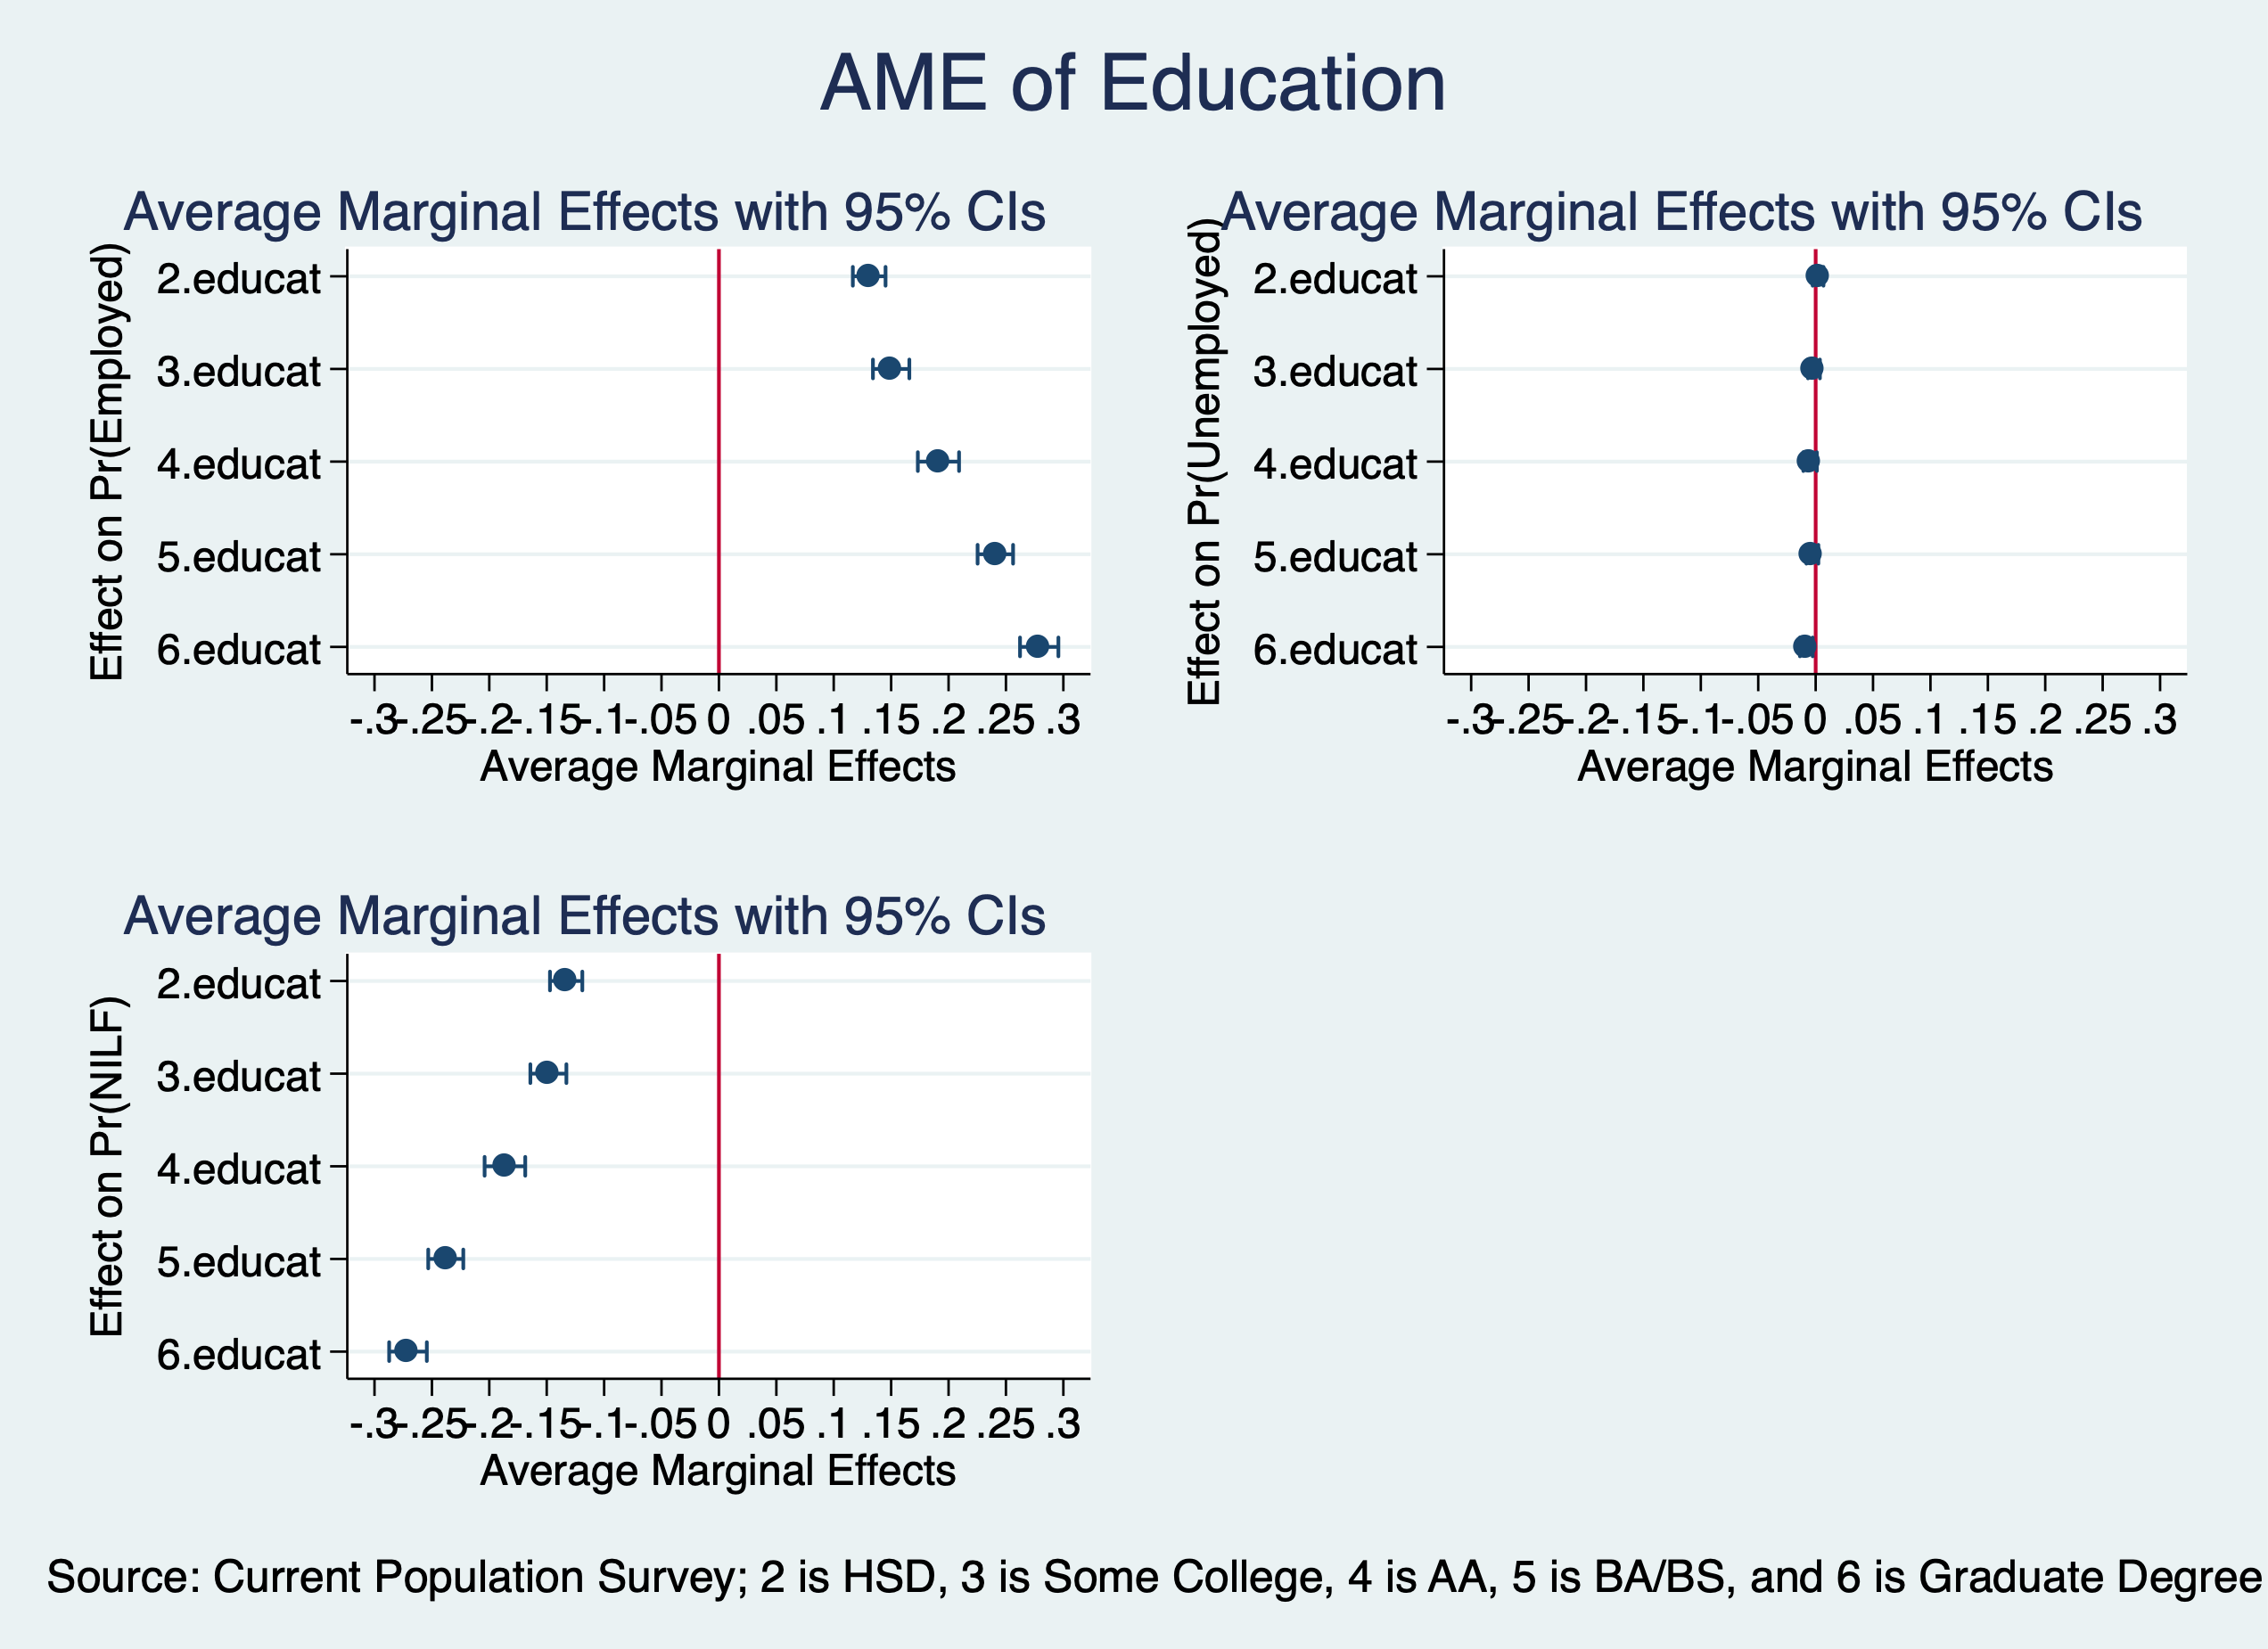
\includegraphics[keepaspectratio]{week8_mnlmeducation.png}}
\caption{Marginal Effects of Education}
\end{figure}

\begin{Shaded}
\begin{Highlighting}[]
\KeywordTok{graph} \KeywordTok{drop}\NormalTok{ Employed Unemployed NILF}
\end{Highlighting}
\end{Shaded}

\subsubsection*{Potential Experience}\label{potential-experience}
\addcontentsline{toc}{subsubsection}{Potential Experience}

For Employed

\begin{Shaded}
\begin{Highlighting}[]
\NormalTok{margins, }\KeywordTok{dydx}\NormalTok{(}\FunctionTok{exp}\NormalTok{) }\FunctionTok{at}\NormalTok{(}\FunctionTok{exp}\NormalTok{=(0(2)60)) }\KeywordTok{predict}\NormalTok{(outcome(1)) }
\KeywordTok{quietly}\NormalTok{ marginsplot, allsimplelabels }\BaseNTok{name}\NormalTok{(Employed) }\BaseNTok{ytitle}\NormalTok{(}\StringTok{"Effect on Pr(Employed)"}\NormalTok{) }\BaseNTok{xtitle}\NormalTok{(}\StringTok{"Average Marginal Effects"}\NormalTok{)}
\end{Highlighting}
\end{Shaded}

\begin{verbatim}
Average marginal effects                        Number of obs     =     41,599
Model VCE    : OIM

Expression   : Pr(laborforcestatus==Employed), predict(outcome(1))
dy/dx w.r.t. : exp

1._at        : exp             =           0

2._at        : exp             =           2

3._at        : exp             =           4

4._at        : exp             =           6

5._at        : exp             =           8

6._at        : exp             =          10

7._at        : exp             =          12

8._at        : exp             =          14

9._at        : exp             =          16

10._at       : exp             =          18

11._at       : exp             =          20

12._at       : exp             =          22

13._at       : exp             =          24

14._at       : exp             =          26

15._at       : exp             =          28

16._at       : exp             =          30

17._at       : exp             =          32

18._at       : exp             =          34

19._at       : exp             =          36

20._at       : exp             =          38

21._at       : exp             =          40

22._at       : exp             =          42

23._at       : exp             =          44

24._at       : exp             =          46

25._at       : exp             =          48

26._at       : exp             =          50

27._at       : exp             =          52

28._at       : exp             =          54

29._at       : exp             =          56

30._at       : exp             =          58

31._at       : exp             =          60

------------------------------------------------------------------------------
             |            Delta-method
             |      dy/dx   Std. Err.      z    P>|z|     [95% Conf. Interval]
-------------+----------------------------------------------------------------
exp          |
         _at |
          1  |   .0119199   .0001127   105.73   0.000     .0116989    .0121408
          2  |   .0130781   .0001155   113.28   0.000     .0128519    .0133044
          3  |    .013976   .0001461    95.64   0.000     .0136896    .0142625
          4  |   .0145643   .0001796    81.10   0.000     .0142123    .0149163
          5  |   .0148298   .0002035    72.86   0.000     .0144308    .0152287
          6  |   .0147942    .000215    68.83   0.000     .0143729    .0152155
          7  |   .0145067   .0002152    67.40   0.000     .0140849    .0149285
          8  |   .0140316   .0002075    67.61   0.000     .0136249    .0144384
          9  |   .0134367   .0001953    68.81   0.000      .013054    .0138195
         10  |   .0127838   .0001811    70.60   0.000     .0124289    .0131387
         11  |   .0121231   .0001667    72.73   0.000     .0117965    .0124498
         12  |   .0114913    .000153    75.12   0.000     .0111915    .0117912
         13  |   .0109121   .0001403    77.76   0.000     .0106371    .0111872
         14  |   .0103981   .0001289    80.69   0.000     .0101455    .0106507
         15  |   .0099532   .0001186    83.95   0.000     .0097208    .0101855
         16  |   .0095751   .0001094    87.52   0.000     .0093606    .0097895
         17  |   .0092574   .0001014    91.30   0.000     .0090586    .0094561
         18  |   .0089913   .0000945    95.12   0.000      .008806    .0091766
         19  |   .0087672   .0000887    98.80   0.000     .0085933    .0089411
         20  |   .0085751   .0000839   102.22   0.000     .0084107    .0087395
         21  |   .0084059   .0000798   105.34   0.000     .0082495    .0085623
         22  |   .0082513   .0000762   108.24   0.000     .0081019    .0084007
         23  |   .0081038   .0000729   111.13   0.000     .0079609    .0082468
         24  |   .0079576   .0000697   114.23   0.000      .007821    .0080941
         25  |   .0078075   .0000663   117.83   0.000     .0076776    .0079373
         26  |   .0076498   .0000626   122.19   0.000     .0075271    .0077725
         27  |   .0074817   .0000586   127.62   0.000     .0073668    .0075967
         28  |   .0073016   .0000543   134.46   0.000     .0071952    .0074081
         29  |   .0071087   .0000497   143.16   0.000     .0070113     .007206
         30  |   .0069031   .0000447   154.27   0.000     .0068154    .0069908
         31  |   .0066862   .0000397   168.35   0.000     .0066084    .0067641
------------------------------------------------------------------------------
\end{verbatim}

For Not in the Labor Force

\begin{Shaded}
\begin{Highlighting}[]
\NormalTok{margins, }\KeywordTok{dydx}\NormalTok{(}\FunctionTok{exp}\NormalTok{) }\FunctionTok{at}\NormalTok{(}\FunctionTok{exp}\NormalTok{=(0(2)60)) }\KeywordTok{predict}\NormalTok{(outcome(3))}
\KeywordTok{quietly}\NormalTok{ marginsplot, allsimplelabels }\BaseNTok{name}\NormalTok{(NILF) }\BaseNTok{ytitle}\NormalTok{(}\StringTok{"Effect on Pr(NILF)"}\NormalTok{) }\BaseNTok{xtitle}\NormalTok{(}\StringTok{"Average Marginal Effects"}\NormalTok{)}
\end{Highlighting}
\end{Shaded}

\begin{verbatim}
Average marginal effects                        Number of obs     =     41,599
Model VCE    : OIM

Expression   : Pr(laborforcestatus==NILF), predict(outcome(3))
dy/dx w.r.t. : exp

1._at        : exp             =           0

2._at        : exp             =           2

3._at        : exp             =           4

4._at        : exp             =           6

5._at        : exp             =           8

6._at        : exp             =          10

7._at        : exp             =          12

8._at        : exp             =          14

9._at        : exp             =          16

10._at       : exp             =          18

11._at       : exp             =          20

12._at       : exp             =          22

13._at       : exp             =          24

14._at       : exp             =          26

15._at       : exp             =          28

16._at       : exp             =          30

17._at       : exp             =          32

18._at       : exp             =          34

19._at       : exp             =          36

20._at       : exp             =          38

21._at       : exp             =          40

22._at       : exp             =          42

23._at       : exp             =          44

24._at       : exp             =          46

25._at       : exp             =          48

26._at       : exp             =          50

27._at       : exp             =          52

28._at       : exp             =          54

29._at       : exp             =          56

30._at       : exp             =          58

31._at       : exp             =          60

------------------------------------------------------------------------------
             |            Delta-method
             |      dy/dx   Std. Err.      z    P>|z|     [95% Conf. Interval]
-------------+----------------------------------------------------------------
exp          |
         _at |
          1  |  -.0125848   .0001155  -108.97   0.000    -.0128111   -.0123584
          2  |  -.0137412   .0001266  -108.55   0.000    -.0139893    -.013493
          3  |  -.0146118    .000159   -91.88   0.000    -.0149235   -.0143001
          4  |  -.0151489   .0001885   -80.35   0.000    -.0155185   -.0147794
          5  |  -.0153436   .0002048   -74.91   0.000     -.015745   -.0149421
          6  |  -.0152237   .0002061   -73.87   0.000    -.0156276   -.0148198
          7  |  -.0148454   .0001949   -76.17   0.000    -.0152274   -.0144634
          8  |  -.0142796   .0001756   -81.30   0.000    -.0146238   -.0139353
          9  |  -.0135992   .0001528   -89.00   0.000    -.0138986   -.0132997
         10  |  -.0128695   .0001299   -99.06   0.000    -.0131241   -.0126148
         11  |  -.0121426   .0001093  -111.07   0.000    -.0123569   -.0119284
         12  |  -.0114558   .0000922  -124.29   0.000    -.0116365   -.0112752
         13  |  -.0108322   .0000787  -137.62   0.000    -.0109865   -.0106779
         14  |  -.0102833   .0000686  -149.81   0.000    -.0104178   -.0101487
         15  |  -.0098117   .0000614  -159.70   0.000    -.0099321   -.0096913
         16  |  -.0094137   .0000566  -166.42   0.000    -.0095246   -.0093028
         17  |  -.0090816   .0000536  -169.49   0.000    -.0091866   -.0089766
         18  |  -.0088055   .0000521  -169.01   0.000    -.0089076   -.0087033
         19  |  -.0085745   .0000517  -165.70   0.000    -.0086759   -.0084731
         20  |   -.008378   .0000521  -160.73   0.000    -.0084802   -.0082759
         21  |  -.0082063   .0000528  -155.31   0.000    -.0083098   -.0081027
         22  |  -.0080503   .0000535  -150.38   0.000    -.0081552   -.0079453
         23  |  -.0079024   .0000539  -146.55   0.000    -.0080081   -.0077967
         24  |  -.0077563   .0000538  -144.13   0.000    -.0078617   -.0076508
         25  |  -.0076067   .0000531  -143.27   0.000    -.0077108   -.0075027
         26  |  -.0074499   .0000517  -144.07   0.000    -.0075512   -.0073485
         27  |  -.0072829   .0000497  -146.60   0.000    -.0073802   -.0071855
         28  |   -.007104    .000047  -151.07   0.000    -.0071962   -.0070118
         29  |  -.0069124   .0000438  -157.78   0.000    -.0069983   -.0068266
         30  |  -.0067085   .0000401  -167.14   0.000    -.0067872   -.0066298
         31  |  -.0064935   .0000362  -179.60   0.000    -.0065643   -.0064226
------------------------------------------------------------------------------
\end{verbatim}

Combine Graphs

\begin{Shaded}
\begin{Highlighting}[]
\KeywordTok{graph} \BaseNTok{combine}\NormalTok{ Employed NILF, }\BaseNTok{ycommon} \BaseNTok{title}\NormalTok{(}\StringTok{"AME of Potential Experience"}\NormalTok{) }
\KeywordTok{graph} \KeywordTok{export} \StringTok{"/Users/Sam/Desktop/Econ 645/Stata/week8\_mnlmexp.png"}\NormalTok{, }\KeywordTok{replace}
\end{Highlighting}
\end{Shaded}

\begin{figure}
\centering
\pandocbounded{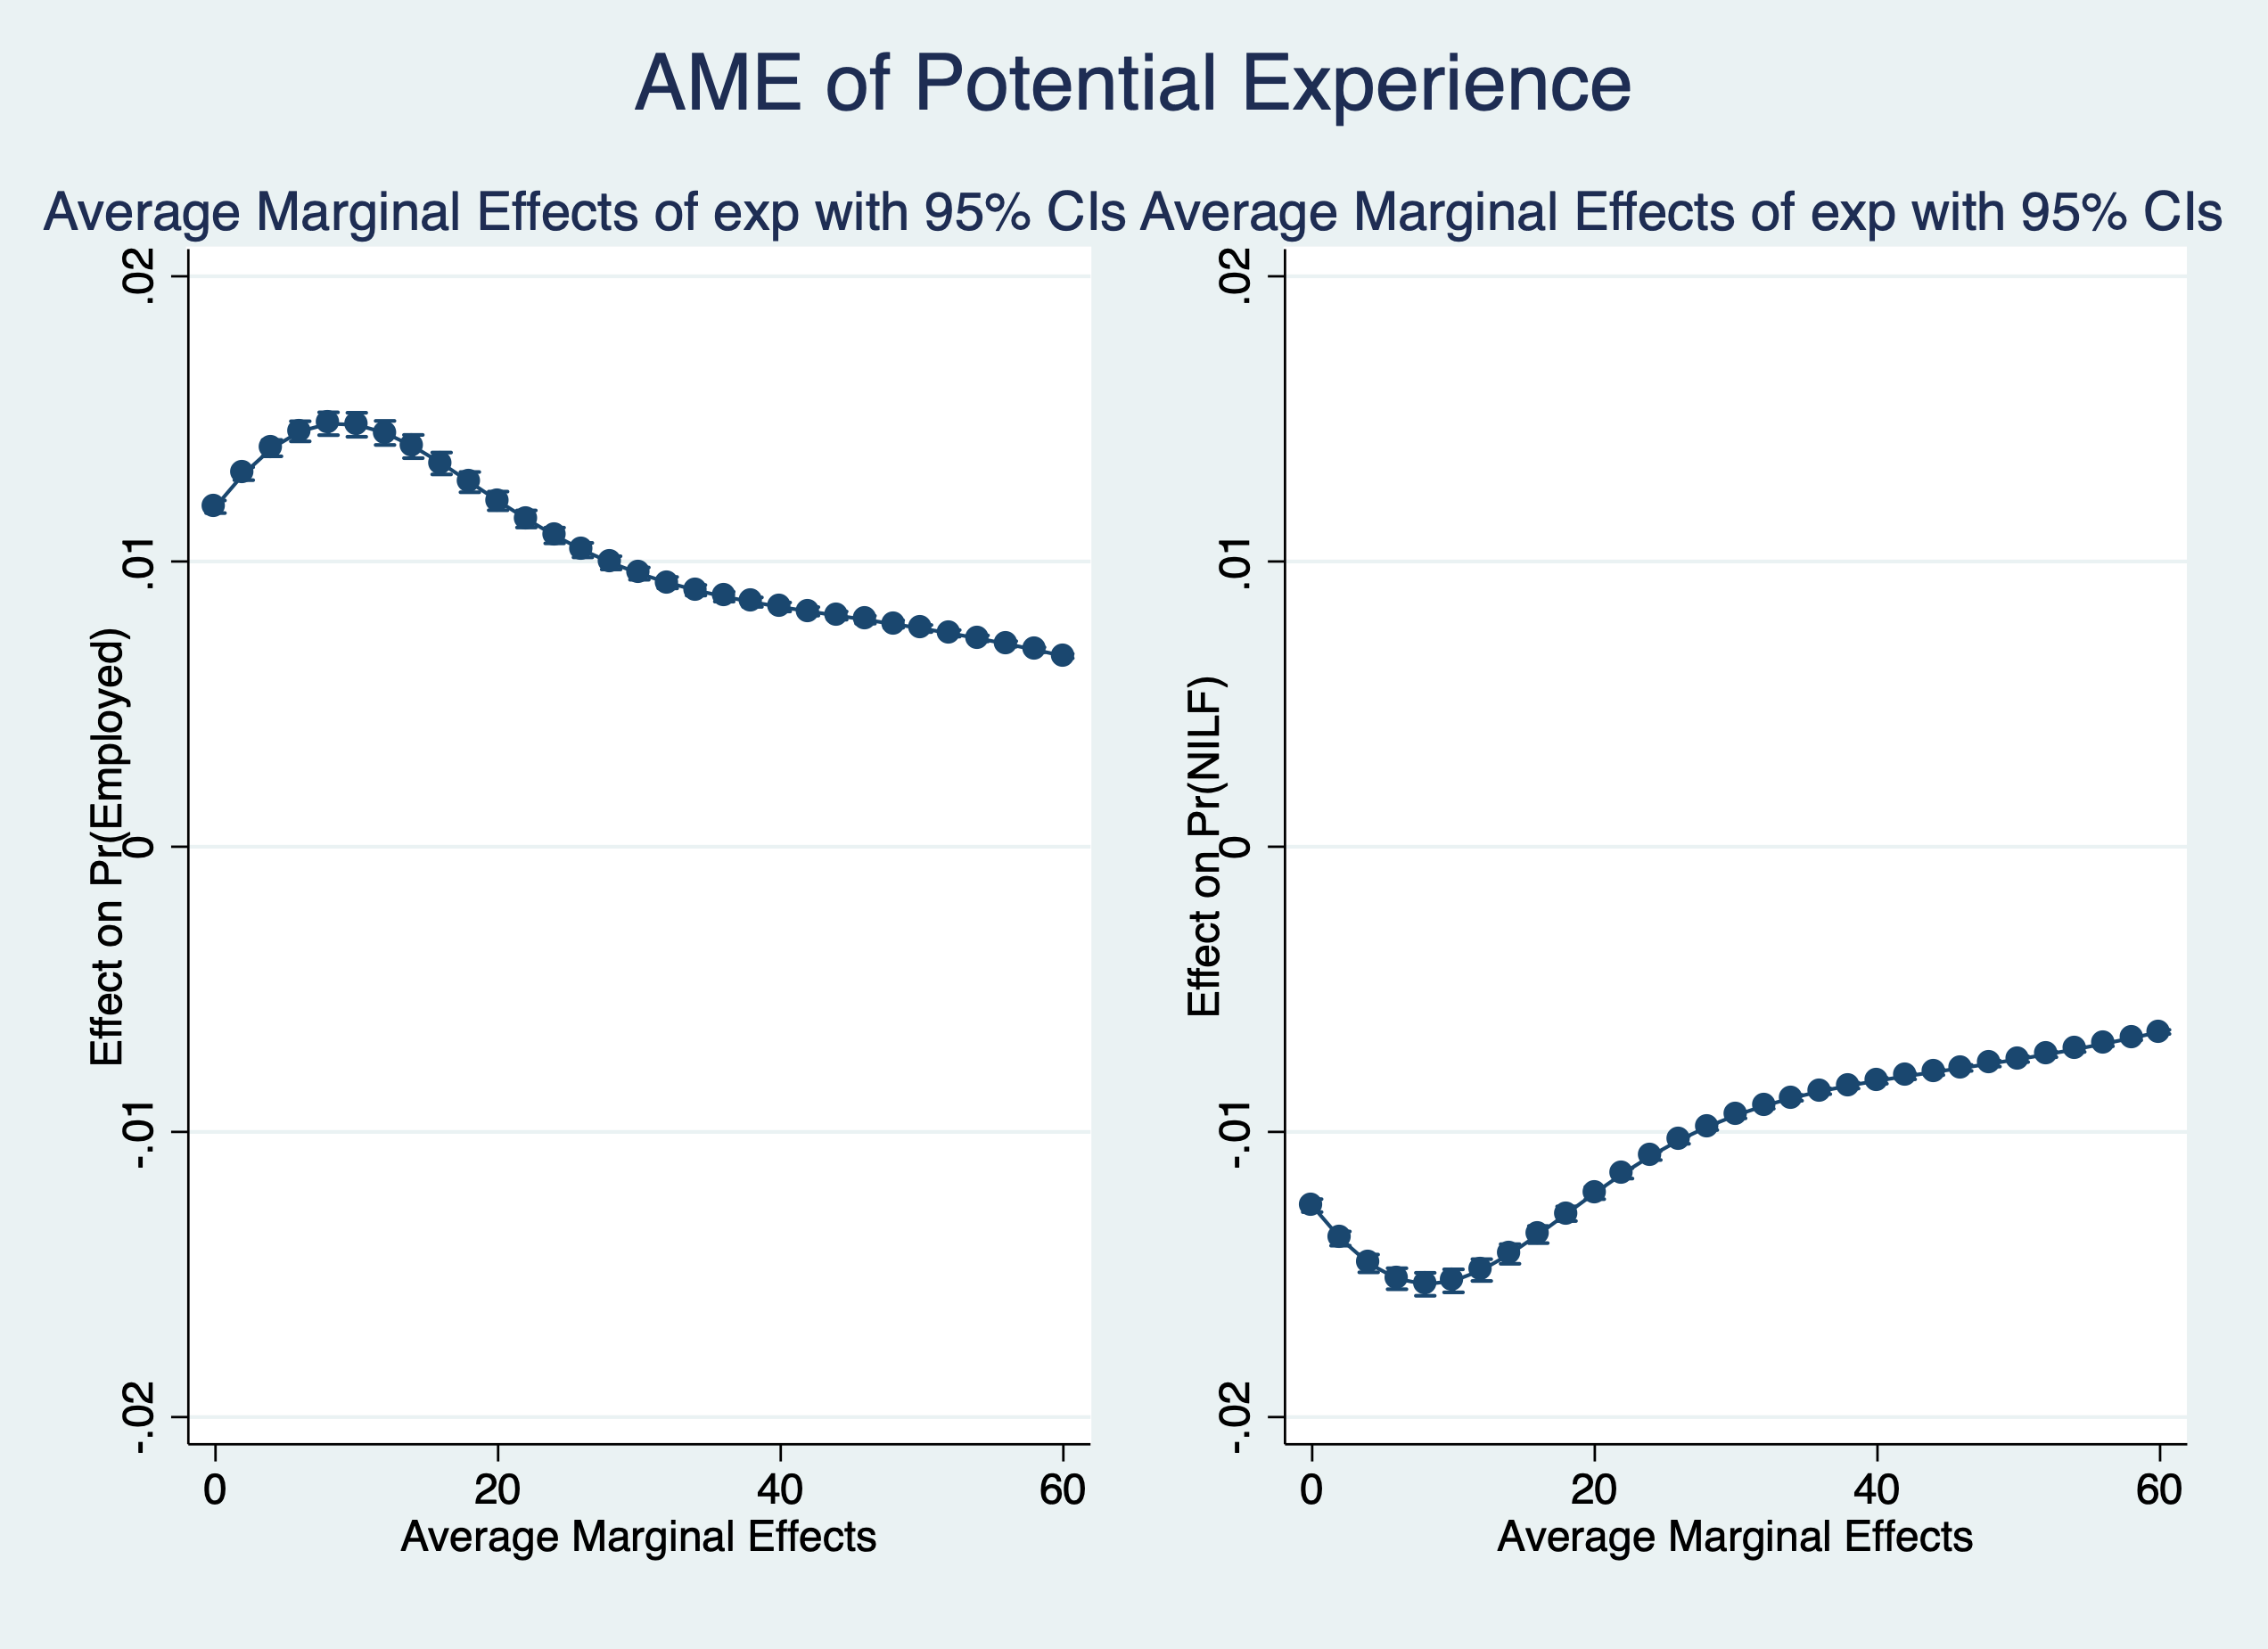
\includegraphics[keepaspectratio]{week8_mnlmexp.png}}
\caption{Marginal Effects of Potential Experience}
\end{figure}

\begin{Shaded}
\begin{Highlighting}[]
\KeywordTok{graph} \KeywordTok{drop}\NormalTok{ Employed NILF}
\end{Highlighting}
\end{Shaded}

\subsection{We can use coefplot with margins with eststo}\label{we-can-use-coefplot-with-margins-with-eststo}

\begin{Shaded}
\begin{Highlighting}[]
\NormalTok{quilety \{}\KeywordTok{est} \KeywordTok{clear}
\NormalTok{eststo mnlm: }\KeywordTok{quietly} \KeywordTok{mlogit}\NormalTok{ laborforce i.educat }\FunctionTok{exp}\NormalTok{ exp2 i.race\_ethnicity i.female i.metroarea i.}\KeywordTok{union}\NormalTok{ i.marital}
\NormalTok{\}}
\end{Highlighting}
\end{Shaded}

Estimate the average marginal effects. Please note the post option when storing margin results

\begin{Shaded}
\begin{Highlighting}[]
\KeywordTok{quietly}\NormalTok{\{}
\NormalTok{eststo Employed: }\KeywordTok{quietly}\NormalTok{ margins, }\KeywordTok{dydx}\NormalTok{(educat) }\KeywordTok{predict}\NormalTok{(outcome(1)) }\KeywordTok{post}
\KeywordTok{estimates} \KeywordTok{restore}\NormalTok{ mnlm}
\NormalTok{eststo Unemployed: }\KeywordTok{quietly}\NormalTok{ margins, }\KeywordTok{dydx}\NormalTok{(educat) }\KeywordTok{predict}\NormalTok{(outcome(2)) }\KeywordTok{post}
\KeywordTok{estimates} \KeywordTok{restore}\NormalTok{ mnlm}
\NormalTok{eststo NILF: }\KeywordTok{quietly}\NormalTok{ margins, }\KeywordTok{dydx}\NormalTok{(educat) }\KeywordTok{predict}\NormalTok{(outcome(3)) }\KeywordTok{post} 
\NormalTok{\}}
\end{Highlighting}
\end{Shaded}

Use coefplot

\begin{Shaded}
\begin{Highlighting}[]
\NormalTok{coefplot Employed Unemployed NILF, }\CommentTok{///}
\KeywordTok{recast}\NormalTok{(}\BaseNTok{bar}\NormalTok{) barw(0.15) vertical }\CommentTok{///}
\NormalTok{ciopts(}\KeywordTok{recast}\NormalTok{(rcap) }\KeywordTok{color}\NormalTok{(gs8)) citop }\CommentTok{///}
\NormalTok{xlab(1 }\StringTok{"High School"}\NormalTok{ 2 }\StringTok{"Some College"}\NormalTok{ 3 }\StringTok{"Associates"}\NormalTok{ 4 }\StringTok{"Bachelor"}\NormalTok{ 5 }\StringTok{"Graduate"}\NormalTok{) }\CommentTok{///}
\BaseNTok{ytitle}\NormalTok{(}\StringTok{"Average Marginal Effect"}\NormalTok{) }\CommentTok{///}
\BaseNTok{xtitle}\NormalTok{(}\StringTok{"High Level of Education Attained"}\NormalTok{) }\CommentTok{///}
\BaseNTok{title}\NormalTok{(}\StringTok{"MNLM: Probability of Labor Force Status"}\NormalTok{, }\KeywordTok{size}\NormalTok{(*0.7))    }\CommentTok{///}
\BaseNTok{subtitle}\NormalTok{(}\StringTok{"By Education Relative to High School Dropout"}\NormalTok{)    }\CommentTok{///}
\BaseNTok{caption}\NormalTok{(}\StringTok{"Source: Current Population Survey"}\NormalTok{, }\KeywordTok{size}\NormalTok{(*0.75)) }\CommentTok{///}
\BaseNTok{name}\NormalTok{(coefplot3)}
\KeywordTok{graph} \KeywordTok{export} \StringTok{"/Users/Sam/Desktop/Econ 645/Stata/week8\_mnlmcoefplot.png"}\NormalTok{, }\KeywordTok{replace}
\end{Highlighting}
\end{Shaded}

\begin{figure}
\centering
\pandocbounded{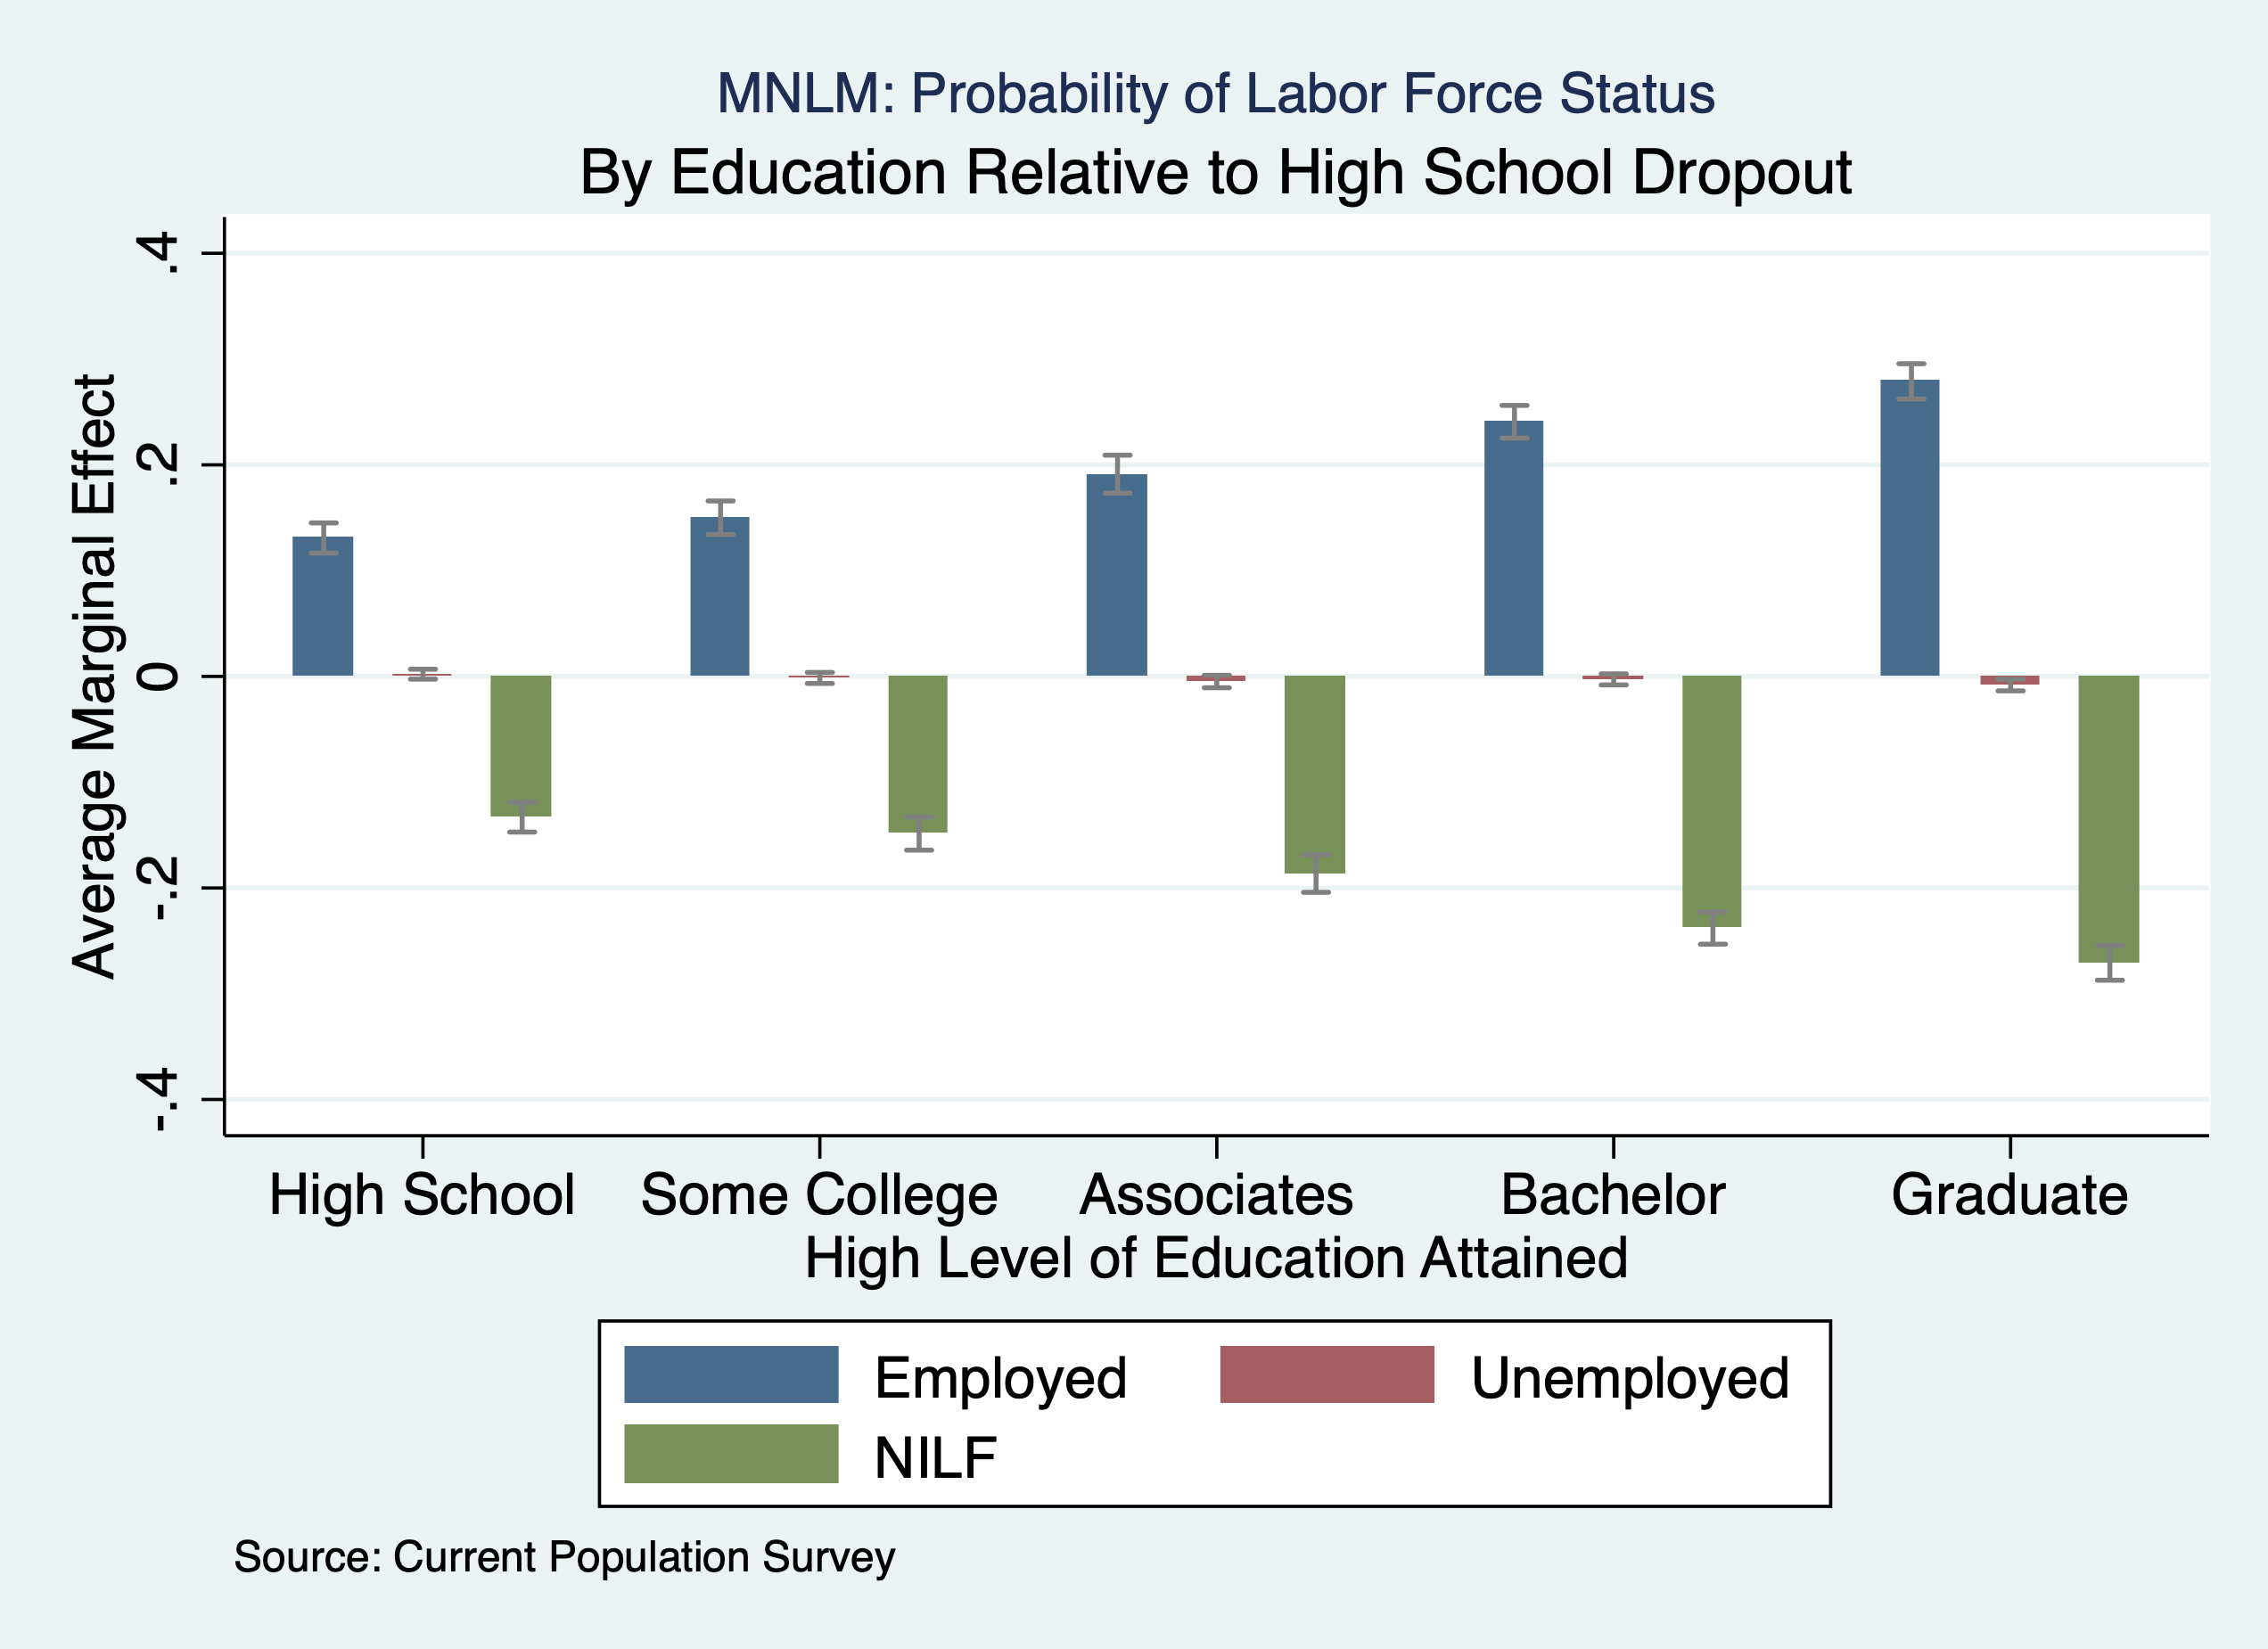
\includegraphics[keepaspectratio]{week8_mnlmcoefplot.png}}
\caption{Using coefplot instead of marginsplot}
\end{figure}

\begin{Shaded}
\begin{Highlighting}[]
\KeywordTok{graph} \KeywordTok{drop}\NormalTok{ coefplot3}
\end{Highlighting}
\end{Shaded}

\chapter{Ordinal Logit}\label{ordinal-logit}

Adapted from Long and Freese (2006)

\section{Compare Ordinal Logit and Binary Logit}\label{compare-ordinal-logit-and-binary-logit}

First, let's inspect the outcome of interest, which is labor force status.

\begin{Shaded}
\begin{Highlighting}[]
\KeywordTok{use} \StringTok{"/Users/Sam/Desktop/Econ 645/Data/binlfp2.dta"}\NormalTok{, }\KeywordTok{clear}
\KeywordTok{tab}\NormalTok{ lfp}
\end{Highlighting}
\end{Shaded}

\begin{verbatim}
(Data from 1976 PSID-T Mroz)


 Paid Labor |
     Force: |
 1=yes 0=no |      Freq.     Percent        Cum.
------------+-----------------------------------
    NotInLF |        325       43.16       43.16
       inLF |        428       56.84      100.00
------------+-----------------------------------
      Total |        753      100.00
\end{verbatim}

Now, let's compare our ordinal logit and binary logit coefficients when the outcome is binary.

\begin{Shaded}
\begin{Highlighting}[]
\KeywordTok{quietly} \KeywordTok{logit}\NormalTok{ lfp k5 k618 age wc hc lwg inc, }\KeywordTok{nolog}
\KeywordTok{estimates} \KeywordTok{store} \KeywordTok{logit}
\KeywordTok{quietly} \KeywordTok{ologit}\NormalTok{ lfp k5 k618 age wc hc lwg inc, }\KeywordTok{nolog}
\KeywordTok{estimates} \KeywordTok{store} \KeywordTok{ologit}
\KeywordTok{estimates} \KeywordTok{table} \KeywordTok{logit} \KeywordTok{ologit}\NormalTok{, b(\%9.3f) t varlabel varwidth(30) equations(1:1)}
\end{Highlighting}
\end{Shaded}

\begin{verbatim}
                      Variable |   logit      ologit    
-------------------------------+------------------------
#1                             |
                    # kids < 6 |    -1.463      -1.463  
                               |     -7.43       -7.43  
                   # kids 6-18 |    -0.065      -0.065  
                               |     -0.95       -0.95  
           Wife's age in years |    -0.063      -0.063  
                               |     -4.92       -4.92  
      Wife College: 1=yes 0=no |     0.807       0.807  
                               |      3.51        3.51  
   Husband College: 1=yes 0=no |     0.112       0.112  
                               |      0.54        0.54  
 Log of wife's estimated wages |     0.605       0.605  
                               |      4.01        4.01  
Family income excluding wife's |    -0.034      -0.034  
                               |     -4.20       -4.20  
                      Constant |     3.182              
                               |      4.94              
-------------------------------+------------------------
cut1                           |
                      Constant |                -3.182  
                               |                 -4.94  
--------------------------------------------------------
                                             legend: b/t
\end{verbatim}

The coefficients are the same between the binary logit and the ordinal logit. The difference here is that the ordinal logit has a cut point and assumes an interept of 0. The cutpoint and the intercept for binary logit are the same in absolute terms.

\section{Example of Ordinal Dependent Variable}\label{example-of-ordinal-dependent-variable}

\begin{Shaded}
\begin{Highlighting}[]
\KeywordTok{use} \StringTok{"/Users/Sam/Desktop/Econ 645/Data/ordwarm2.dta"}\NormalTok{, }\KeywordTok{clear}
\KeywordTok{describe}\NormalTok{ warm yr89 male }\BaseNTok{white}\NormalTok{ age ed prst}
\end{Highlighting}
\end{Shaded}

\begin{verbatim}
(77 & 89 General Social Survey)

              storage   display    value
variable name   type    format     label      variable label
----------------------------------------------------------------------------------------------------------------------
warm            byte    %10.0g     SD2SA      Mom can have warm relations with child
yr89            byte    %10.0g     yrlbl      Survey year: 1=1989 0=1977
male            byte    %10.0g     sexlbl     Gender: 1=male 0=female
white           byte    %10.0g     racelbl    Race: 1=white 0=not white
age             byte    %10.0g                Age in years
ed              byte    %10.0g                Years of education
prst            byte    %10.0g                Occupational prestige
\end{verbatim}

\begin{Shaded}
\begin{Highlighting}[]
\KeywordTok{summarize}\NormalTok{ warm yr89 male }\BaseNTok{white}\NormalTok{ age ed prst}
\end{Highlighting}
\end{Shaded}

\begin{verbatim}
    Variable |        Obs        Mean    Std. Dev.       Min        Max
-------------+---------------------------------------------------------
        warm |      2,293    2.607501    .9282156          1          4
        yr89 |      2,293    .3986044    .4897178          0          1
        male |      2,293    .4648932    .4988748          0          1
       white |      2,293    .8765809    .3289894          0          1
         age |      2,293    44.93546    16.77903         18         89
-------------+---------------------------------------------------------
          ed |      2,293    12.21805    3.160827          0         20
        prst |      2,293    39.58526    14.49226         12         82
\end{verbatim}

Our outcome is the the survey results for people's opinion for a working mother

\begin{Shaded}
\begin{Highlighting}[]
\KeywordTok{tab}\NormalTok{ warm}
\end{Highlighting}
\end{Shaded}

\begin{verbatim}
    Mom can |
  have warm |
  relations |
 with child |      Freq.     Percent        Cum.
------------+-----------------------------------
         SD |        297       12.95       12.95
          D |        723       31.53       44.48
          A |        856       37.33       81.81
         SA |        417       18.19      100.00
------------+-----------------------------------
      Total |      2,293      100.00
\end{verbatim}

We will run our ordinal logit by regressing opinion's on working mother's warm onto gender, race,
age, survey year, education in years, and occupational prestige.

\[ warm_{i,t} = \beta_1 male_i + \beta_2 race_i + \beta_3 age_{i,t} + \beta_4 edu_{i,t} + \beta_5 prestige_{i,t} + \beta_6 y89_t + \varepsilon_{i,t} \]

\begin{Shaded}
\begin{Highlighting}[]
\KeywordTok{ologit}\NormalTok{ warm yr89 male }\BaseNTok{white}\NormalTok{ age ed prst, }\KeywordTok{nolog}
\end{Highlighting}
\end{Shaded}

\begin{verbatim}
Ordered logistic regression                     Number of obs     =      2,293
                                                LR chi2(6)        =     301.72
                                                Prob > chi2       =     0.0000
Log likelihood = -2844.9123                     Pseudo R2         =     0.0504

------------------------------------------------------------------------------
        warm |      Coef.   Std. Err.      z    P>|z|     [95% Conf. Interval]
-------------+----------------------------------------------------------------
        yr89 |   .5239025   .0798989     6.56   0.000     .3673036    .6805014
        male |  -.7332997   .0784827    -9.34   0.000     -.887123   -.5794765
       white |  -.3911595   .1183808    -3.30   0.001    -.6231816   -.1591373
         age |  -.0216655   .0024683    -8.78   0.000    -.0265032   -.0168278
          ed |   .0671728    .015975     4.20   0.000     .0358624    .0984831
        prst |   .0060727   .0032929     1.84   0.065    -.0003813    .0125267
-------------+----------------------------------------------------------------
       /cut1 |  -2.465362   .2389128                     -2.933622   -1.997102
       /cut2 |   -.630904   .2333156                     -1.088194   -.1736138
       /cut3 |   1.261854    .234018                      .8031871    1.720521
------------------------------------------------------------------------------
\end{verbatim}

We have three cutpoints \[ \tau_1 = -2.47, \tau_2 = -0.63, \tau_3 = 1.26 \]

\section{Test Proportional Odds Assumption}\label{test-proportional-odds-assumption}

We have our two tests for testing the proportional odds assumption
1. Approximate Likelihood Ratio Test
2. Wald Test

\subsection{Approximate Likelihood Ratio Test}\label{approximate-likelihood-ratio-test}

We use the \emph{omodel} command to run an Approximate Likelihood Ratio Test

\begin{Shaded}
\begin{Highlighting}[]
\NormalTok{omodel }\KeywordTok{logit}\NormalTok{ warm yr89 male }\BaseNTok{white}\NormalTok{ age ed prst}
\end{Highlighting}
\end{Shaded}

\begin{verbatim}
Iteration 0:   log likelihood = -2995.7704
Iteration 1:   log likelihood = -2846.4532
Iteration 2:   log likelihood = -2844.9142
Iteration 3:   log likelihood = -2844.9123

Ordered logit estimates                           Number of obs   =       2293
                                                  LR chi2(6)      =     301.72
                                                  Prob > chi2     =     0.0000
Log likelihood = -2844.9123                       Pseudo R2       =     0.0504

------------------------------------------------------------------------------
        warm |      Coef.   Std. Err.      z    P>|z|     [95% Conf. Interval]
-------------+----------------------------------------------------------------
        yr89 |   .5239025   .0798988     6.56   0.000     .3673037    .6805013
        male |  -.7332997   .0784827    -9.34   0.000    -.8871229   -.5794766
       white |  -.3911595   .1183808    -3.30   0.001    -.6231815   -.1591374
         age |  -.0216655   .0024683    -8.78   0.000    -.0265032   -.0168278
          ed |   .0671728    .015975     4.20   0.000     .0358624    .0984831
        prst |   .0060727   .0032929     1.84   0.065    -.0003813    .0125267
-------------+----------------------------------------------------------------
       _cut1 |  -2.465362   .2389126          (Ancillary parameters)
       _cut2 |   -.630904   .2333155 
       _cut3 |   1.261854   .2340179 
------------------------------------------------------------------------------

Approximate likelihood-ratio test of proportionality of odds
across response categories:
         chi2(12) =     48.91
       Prob > chi2 =    0.0000
\end{verbatim}

With the oparallel package

\begin{Shaded}
\begin{Highlighting}[]
\KeywordTok{help}\NormalTok{ oparallel}
\KeywordTok{quietly}\NormalTok{ omodel }\KeywordTok{logit}\NormalTok{ warm yr89 male }\BaseNTok{white}\NormalTok{ age ed prst}
\NormalTok{oparallel, lr}
\end{Highlighting}
\end{Shaded}

\begin{verbatim}
Test of the parallel regression assumption

                 |   Chi2     df  P>Chi2
-----------------+----------------------
likelihood ratio |   49.2     12   0.000
\end{verbatim}

We reject the null hypothesis that the coefficients are the same across \(1,...,J-1\) equations at the 0.1\% level.

\subsection{Wald Test}\label{wald-test}

We use the \emph{brant} command for the Wald Test

\begin{Shaded}
\begin{Highlighting}[]
\KeywordTok{quietly} \KeywordTok{ologit}\NormalTok{ warm yr89 male }\BaseNTok{white}\NormalTok{ age ed prst, }\KeywordTok{nolog}
\NormalTok{oparallel, lr}
\end{Highlighting}
\end{Shaded}

\begin{Shaded}
\begin{Highlighting}[]
\KeywordTok{quietly} \KeywordTok{use} \StringTok{"/Users/Sam/Desktop/Econ 645/Data/ordwarm2.dta"}\NormalTok{, }\KeywordTok{clear}
\KeywordTok{quietly} \KeywordTok{ologit}\NormalTok{ warm yr89 male }\BaseNTok{white}\NormalTok{ age ed prst, }\KeywordTok{nolog}
\NormalTok{oparallel, lr}
\end{Highlighting}
\end{Shaded}

We reject the null hypothesis that the coefficients are the same across \(1,...,J-1\) equations at the 0.1\% level.

\section{Interpretation}\label{interpretation}

\subsection{Odds Ratios}\label{odds-ratios-1}

\begin{Shaded}
\begin{Highlighting}[]
\KeywordTok{ologit}\NormalTok{ warm yr89 male }\BaseNTok{white}\NormalTok{ age ed prst, }\KeywordTok{or}
\NormalTok{oparallel, lr}
\NormalTok{listcoef, }\KeywordTok{help}
\NormalTok{listcoef, }\KeywordTok{help} \KeywordTok{percent}
\end{Highlighting}
\end{Shaded}

\begin{verbatim}
Iteration 0:   log likelihood = -2995.7704  
Iteration 1:   log likelihood = -2846.4532  
Iteration 2:   log likelihood = -2844.9142  
Iteration 3:   log likelihood = -2844.9123  
Iteration 4:   log likelihood = -2844.9123  

Ordered logistic regression                     Number of obs     =      2,293
                                                LR chi2(6)        =     301.72
                                                Prob > chi2       =     0.0000
Log likelihood = -2844.9123                     Pseudo R2         =     0.0504

------------------------------------------------------------------------------
        warm | Odds Ratio   Std. Err.      z    P>|z|     [95% Conf. Interval]
-------------+----------------------------------------------------------------
        yr89 |   1.688605   .1349176     6.56   0.000     1.443836    1.974868
        male |   .4803214   .0376969    -9.34   0.000     .4118389    .5601916
       white |   .6762723   .0800577    -3.30   0.001     .5362356    .8528792
         age |   .9785675   .0024154    -8.78   0.000     .9738449     .983313
          ed |    1.06948   .0170849     4.20   0.000     1.036513    1.103496
        prst |   1.006091    .003313     1.84   0.065     .9996188    1.012605
-------------+----------------------------------------------------------------
       /cut1 |  -2.465362   .2389128                     -2.933622   -1.997102
       /cut2 |   -.630904   .2333156                     -1.088194   -.1736138
       /cut3 |   1.261854    .234018                      .8031871    1.720521
------------------------------------------------------------------------------


ologit (N=2293): Factor Change in Odds 

  Odds of: >m vs <=m

------------------------------------------------------------------
    warm |      b         z     P>|z|    e^b    e^bStdX      SDofX
---------+--------------------------------------------------------
    yr89 |   0.52390    6.557   0.000   1.6886   1.2925     0.4897
    male |  -0.73330   -9.343   0.000   0.4803   0.6936     0.4989
   white |  -0.39116   -3.304   0.001   0.6763   0.8792     0.3290
     age |  -0.02167   -8.778   0.000   0.9786   0.6952    16.7790
      ed |   0.06717    4.205   0.000   1.0695   1.2365     3.1608
    prst |   0.00607    1.844   0.065   1.0061   1.0920    14.4923
------------------------------------------------------------------
       b = raw coefficient
       z = z-score for test of b=0
   P>|z| = p-value for z-test
     e^b = exp(b) = factor change in odds for unit increase in X
 e^bStdX = exp(b*SD of X) = change in odds for SD increase in X
   SDofX = standard deviation of X


ologit (N=2293): Percentage Change in Odds 

  Odds of: >m vs <=m

------------------------------------------------------------------
    warm |      b         z     P>|z|      %      %StdX      SDofX
---------+--------------------------------------------------------
    yr89 |   0.52390    6.557   0.000     68.9     29.2     0.4897
    male |  -0.73330   -9.343   0.000    -52.0    -30.6     0.4989
   white |  -0.39116   -3.304   0.001    -32.4    -12.1     0.3290
     age |  -0.02167   -8.778   0.000     -2.1    -30.5    16.7790
      ed |   0.06717    4.205   0.000      6.9     23.7     3.1608
    prst |   0.00607    1.844   0.065      0.6      9.2    14.4923
------------------------------------------------------------------
       b = raw coefficient
       z = z-score for test of b=0
   P>|z| = p-value for z-test
       % = percent change in odds for unit increase in X
   %StdX = percent change in odds for SD increase in X
   SDofX = standard deviation of X
\end{verbatim}

For a 1-year increase in education , the odds of a \textbf{positive attitude} towards working mothers increase by a factor of 1.067 or 6.7\%, ceteris paribus.

For a 1-year increase in age, the odds of a \textbf{negative} attitude toward working mothers increase by a factor of \(e^{-(-0.02167)}=1.0219\), ceteris paribus.

For a male, the odds of a \textbf{negative attitude} toward working mothers increase by a factor of \(e^{-(-0.73330)}=2.08\), ceteris paribus

\subsection{Average Marginal Effects}\label{average-marginal-effects-1}

\begin{Shaded}
\begin{Highlighting}[]
\KeywordTok{ologit}\NormalTok{ warm yr89 male }\BaseNTok{white}\NormalTok{ age ed prst, }\KeywordTok{or}

\NormalTok{margins, }\KeywordTok{dydx}\NormalTok{(*) }\KeywordTok{predict}\NormalTok{(outcome(1))}
\NormalTok{margins, }\KeywordTok{dydx}\NormalTok{(*) }\KeywordTok{predict}\NormalTok{(outcome(2))}
\NormalTok{margins, }\KeywordTok{dydx}\NormalTok{(*) }\KeywordTok{predict}\NormalTok{(outcome(3))}
\NormalTok{margins, }\KeywordTok{dydx}\NormalTok{(*) }\KeywordTok{predict}\NormalTok{(outcome(4))}
\end{Highlighting}
\end{Shaded}

\begin{verbatim}
Iteration 0:   log likelihood = -2995.7704  
Iteration 1:   log likelihood = -2846.4532  
Iteration 2:   log likelihood = -2844.9142  
Iteration 3:   log likelihood = -2844.9123  
Iteration 4:   log likelihood = -2844.9123  

Ordered logistic regression                     Number of obs     =      2,293
                                                LR chi2(6)        =     301.72
                                                Prob > chi2       =     0.0000
Log likelihood = -2844.9123                     Pseudo R2         =     0.0504

------------------------------------------------------------------------------
        warm | Odds Ratio   Std. Err.      z    P>|z|     [95% Conf. Interval]
-------------+----------------------------------------------------------------
        yr89 |   1.688605   .1349176     6.56   0.000     1.443836    1.974868
        male |   .4803214   .0376969    -9.34   0.000     .4118389    .5601916
       white |   .6762723   .0800577    -3.30   0.001     .5362356    .8528792
         age |   .9785675   .0024154    -8.78   0.000     .9738449     .983313
          ed |    1.06948   .0170849     4.20   0.000     1.036513    1.103496
        prst |   1.006091    .003313     1.84   0.065     .9996188    1.012605
-------------+----------------------------------------------------------------
       /cut1 |  -2.465362   .2389128                     -2.933622   -1.997102
       /cut2 |   -.630904   .2333156                     -1.088194   -.1736138
       /cut3 |   1.261854    .234018                      .8031871    1.720521
------------------------------------------------------------------------------


Average marginal effects                        Number of obs     =      2,293
Model VCE    : OIM

Expression   : Pr(warm==1), predict(outcome(1))
dy/dx w.r.t. : yr89 male white age ed prst

------------------------------------------------------------------------------
             |            Delta-method
             |      dy/dx   Std. Err.      z    P>|z|     [95% Conf. Interval]
-------------+----------------------------------------------------------------
        yr89 |  -.0557094   .0087921    -6.34   0.000    -.0729416   -.0384771
        male |   .0779757   .0088072     8.85   0.000     .0607139    .0952375
       white |   .0415941   .0127155     3.27   0.001     .0166721    .0665161
         age |   .0023038   .0002754     8.37   0.000     .0017641    .0028435
          ed |  -.0071428   .0017147    -4.17   0.000    -.0105036   -.0037821
        prst |  -.0006457   .0003514    -1.84   0.066    -.0013345     .000043
------------------------------------------------------------------------------


Average marginal effects                        Number of obs     =      2,293
Model VCE    : OIM

Expression   : Pr(warm==2), predict(outcome(2))
dy/dx w.r.t. : yr89 male white age ed prst

------------------------------------------------------------------------------
             |            Delta-method
             |      dy/dx   Std. Err.      z    P>|z|     [95% Conf. Interval]
-------------+----------------------------------------------------------------
        yr89 |  -.0608201   .0091774    -6.63   0.000    -.0788075   -.0428328
        male |   .0851292   .0089196     9.54   0.000     .0676472    .1026112
       white |   .0454099   .0136969     3.32   0.001     .0185644    .0722554
         age |   .0025152   .0002817     8.93   0.000      .001963    .0030673
          ed |  -.0077981     .00185    -4.22   0.000    -.0114241   -.0041722
        prst |   -.000705   .0003818    -1.85   0.065    -.0014533    .0000433
------------------------------------------------------------------------------


Average marginal effects                        Number of obs     =      2,293
Model VCE    : OIM

Expression   : Pr(warm==3), predict(outcome(3))
dy/dx w.r.t. : yr89 male white age ed prst

------------------------------------------------------------------------------
             |            Delta-method
             |      dy/dx   Std. Err.      z    P>|z|     [95% Conf. Interval]
-------------+----------------------------------------------------------------
        yr89 |    .043531   .0069122     6.30   0.000     .0299833    .0570787
        male |  -.0609298   .0067839    -8.98   0.000     -.074226   -.0476336
       white |  -.0325014   .0099733    -3.26   0.001    -.0520487   -.0129541
         age |  -.0018002   .0002138    -8.42   0.000    -.0022193   -.0013811
          ed |   .0055814   .0013342     4.18   0.000     .0029665    .0081963
        prst |   .0005046   .0002752     1.83   0.067    -.0000349    .0010441
------------------------------------------------------------------------------


Average marginal effects                        Number of obs     =      2,293
Model VCE    : OIM

Expression   : Pr(warm==4), predict(outcome(4))
dy/dx w.r.t. : yr89 male white age ed prst

------------------------------------------------------------------------------
             |            Delta-method
             |      dy/dx   Std. Err.      z    P>|z|     [95% Conf. Interval]
-------------+----------------------------------------------------------------
        yr89 |   .0729985   .0111797     6.53   0.000     .0510866    .0949103
        male |   -.102175   .0111936    -9.13   0.000    -.1241141    -.080236
       white |  -.0545026    .016485    -3.31   0.001    -.0868126   -.0221926
         age |  -.0030188   .0003501    -8.62   0.000    -.0037051   -.0023325
          ed |   .0093596   .0022406     4.18   0.000     .0049681    .0137511
        prst |   .0008461   .0004584     1.85   0.065    -.0000522    .0017445
------------------------------------------------------------------------------
\end{verbatim}

\subsection{Marginal Effects at the Average}\label{marginal-effects-at-the-average-1}

\begin{Shaded}
\begin{Highlighting}[]
\KeywordTok{ologit}\NormalTok{ warm yr89 male }\BaseNTok{white}\NormalTok{ age ed prst, }\KeywordTok{or}

\NormalTok{margins, }\KeywordTok{dydx}\NormalTok{(*) atmeans }\KeywordTok{predict}\NormalTok{(outcome(1))}
\NormalTok{margins, }\KeywordTok{dydx}\NormalTok{(*) atmeans }\KeywordTok{predict}\NormalTok{(outcome(2))}
\NormalTok{margins, }\KeywordTok{dydx}\NormalTok{(*) atmeans }\KeywordTok{predict}\NormalTok{(outcome(3))}
\NormalTok{margins, }\KeywordTok{dydx}\NormalTok{(*) atmeans }\KeywordTok{predict}\NormalTok{(outcome(4))}
\end{Highlighting}
\end{Shaded}

\begin{verbatim}
Iteration 0:   log likelihood = -2995.7704  
Iteration 1:   log likelihood = -2846.4532  
Iteration 2:   log likelihood = -2844.9142  
Iteration 3:   log likelihood = -2844.9123  
Iteration 4:   log likelihood = -2844.9123  

Ordered logistic regression                     Number of obs     =      2,293
                                                LR chi2(6)        =     301.72
                                                Prob > chi2       =     0.0000
Log likelihood = -2844.9123                     Pseudo R2         =     0.0504

------------------------------------------------------------------------------
        warm | Odds Ratio   Std. Err.      z    P>|z|     [95% Conf. Interval]
-------------+----------------------------------------------------------------
        yr89 |   1.688605   .1349176     6.56   0.000     1.443836    1.974868
        male |   .4803214   .0376969    -9.34   0.000     .4118389    .5601916
       white |   .6762723   .0800577    -3.30   0.001     .5362356    .8528792
         age |   .9785675   .0024154    -8.78   0.000     .9738449     .983313
          ed |    1.06948   .0170849     4.20   0.000     1.036513    1.103496
        prst |   1.006091    .003313     1.84   0.065     .9996188    1.012605
-------------+----------------------------------------------------------------
       /cut1 |  -2.465362   .2389128                     -2.933622   -1.997102
       /cut2 |   -.630904   .2333156                     -1.088194   -.1736138
       /cut3 |   1.261854    .234018                      .8031871    1.720521
------------------------------------------------------------------------------


Conditional marginal effects                    Number of obs     =      2,293
Model VCE    : OIM

Expression   : Pr(warm==1), predict(outcome(1))
dy/dx w.r.t. : yr89 male white age ed prst
at           : yr89            =    .3986044 (mean)
               male            =    .4648932 (mean)
               white           =    .8765809 (mean)
               age             =    44.93546 (mean)
               ed              =    12.21805 (mean)
               prst            =    39.58526 (mean)

------------------------------------------------------------------------------
             |            Delta-method
             |      dy/dx   Std. Err.      z    P>|z|     [95% Conf. Interval]
-------------+----------------------------------------------------------------
        yr89 |   -.051803   .0081383    -6.37   0.000    -.0677537   -.0358522
        male |   .0725079   .0081294     8.92   0.000     .0565746    .0884413
       white |   .0386775   .0118016     3.28   0.001     .0155468    .0618081
         age |   .0021423   .0002546     8.41   0.000     .0016432    .0026413
          ed |   -.006642   .0015972    -4.16   0.000    -.0097724   -.0035116
        prst |  -.0006005   .0003264    -1.84   0.066    -.0012401    .0000392
------------------------------------------------------------------------------


Conditional marginal effects                    Number of obs     =      2,293
Model VCE    : OIM

Expression   : Pr(warm==2), predict(outcome(2))
dy/dx w.r.t. : yr89 male white age ed prst
at           : yr89            =    .3986044 (mean)
               male            =    .4648932 (mean)
               white           =    .8765809 (mean)
               age             =    44.93546 (mean)
               ed              =    12.21805 (mean)
               prst            =    39.58526 (mean)

------------------------------------------------------------------------------
             |            Delta-method
             |      dy/dx   Std. Err.      z    P>|z|     [95% Conf. Interval]
-------------+----------------------------------------------------------------
        yr89 |  -.0772501   .0122256    -6.32   0.000    -.1012118   -.0532885
        male |   .1081261   .0124796     8.66   0.000     .0836666    .1325855
       white |    .057677    .017613     3.27   0.001     .0231561    .0921979
         age |   .0031946   .0003899     8.19   0.000     .0024304    .0039588
          ed |  -.0099047   .0023955    -4.13   0.000    -.0145999   -.0052095
        prst |  -.0008954   .0004869    -1.84   0.066    -.0018497    .0000588
------------------------------------------------------------------------------


Conditional marginal effects                    Number of obs     =      2,293
Model VCE    : OIM

Expression   : Pr(warm==3), predict(outcome(3))
dy/dx w.r.t. : yr89 male white age ed prst
at           : yr89            =    .3986044 (mean)
               male            =    .4648932 (mean)
               white           =    .8765809 (mean)
               age             =    44.93546 (mean)
               ed              =    12.21805 (mean)
               prst            =    39.58526 (mean)

------------------------------------------------------------------------------
             |            Delta-method
             |      dy/dx   Std. Err.      z    P>|z|     [95% Conf. Interval]
-------------+----------------------------------------------------------------
        yr89 |   .0582103   .0096161     6.05   0.000     .0393631    .0770575
        male |  -.0814762   .0099979    -8.15   0.000    -.1010717   -.0618807
       white |  -.0434613   .0134313    -3.24   0.001    -.0697862   -.0171364
         age |  -.0024072   .0003126    -7.70   0.000    -.0030199   -.0017945
          ed |   .0074635   .0018362     4.06   0.000     .0038645    .0110625
        prst |   .0006747   .0003683     1.83   0.067    -.0000472    .0013967
------------------------------------------------------------------------------


Conditional marginal effects                    Number of obs     =      2,293
Model VCE    : OIM

Expression   : Pr(warm==4), predict(outcome(4))
dy/dx w.r.t. : yr89 male white age ed prst
at           : yr89            =    .3986044 (mean)
               male            =    .4648932 (mean)
               white           =    .8765809 (mean)
               age             =    44.93546 (mean)
               ed              =    12.21805 (mean)
               prst            =    39.58526 (mean)

------------------------------------------------------------------------------
             |            Delta-method
             |      dy/dx   Std. Err.      z    P>|z|     [95% Conf. Interval]
-------------+----------------------------------------------------------------
        yr89 |   .0708428   .0109038     6.50   0.000     .0494718    .0922139
        male |  -.0991578   .0109073    -9.09   0.000    -.1205356   -.0777799
       white |  -.0528931   .0160474    -3.30   0.001    -.0843454   -.0214409
         age |  -.0029296     .00034    -8.62   0.000    -.0035961   -.0022632
          ed |   .0090832   .0021702     4.19   0.000     .0048296    .0133368
        prst |   .0008212   .0004455     1.84   0.065    -.0000519    .0016943
------------------------------------------------------------------------------
\end{verbatim}

\chapter{Reshape}\label{reshape}

From my experience, I feel that understanding and mastering the reshape command is invaluable. This is especially true when working with panel data. Panel data should not be used in a wide format. Panel data should be in a long format where you can use the xtset unit time command. After the xtset is established you can easily add lags or differences with the l.var or d.var

It is also helpful in terms of merging datasets. A lot of time if I'm merging BLS data, such as state unemployment, or inflation rates, I need to reshape the BLS data from wide to long to I can merge m:1

I typically work in long formats, but reshaping to wide formats does have its benefits. I find wide formats are helpful for people who work in excel, especially when years are across columns.

\section{Wide and Long Datasets}\label{wide-and-long-datasets}

We have two types of datasets: wide and long

\subsection*{Wide Format}\label{wide-format}
\addcontentsline{toc}{subsection}{Wide Format}

Our wide datasets typically include years or variables types spread out across
the columns.

\begin{Shaded}
\begin{Highlighting}[]
\NormalTok{cd }\StringTok{"/Users/Sam/Desktop/Econ 645/Data/Mitchell"}
\KeywordTok{use}\NormalTok{ cardio\_wide, }\KeywordTok{clear}
\KeywordTok{describe}
\end{Highlighting}
\end{Shaded}

\begin{verbatim}
/Users/Sam/Desktop/Econ 645/Data/Mitchell



Contains data from cardio_wide.dta
  obs:             6                          
 vars:            12                          22 Dec 2009 20:43
 size:           120                          
----------------------------------------------------------------------------------------------------------------------
              storage   display    value
variable name   type    format     label      variable label
----------------------------------------------------------------------------------------------------------------------
id              byte    %3.0f                 ID of person
age             byte    %3.0f                 Age of person
bp1             int     %3.0f                 Blood pressure systolic Trial 1
bp2             int     %3.0f                 Blood pressure systolic Trial 2
bp3             int     %3.0f                 Blood pressure systolic Trial 3
bp4             int     %3.0f                 Blood pressure systolic Trial 4
bp5             int     %3.0f                 Blood pressure systolic Trial 5
pl1             int     %3.0f                 Pulse: Trial 1
pl2             byte    %3.0f                 Pulse: Trial 2
pl3             int     %3.0f                 Pulse: Trial 3
pl4             int     %3.0f                 Pulse: Trial 4
pl5             byte    %3.0f                 Pulse: Trial 5
----------------------------------------------------------------------------------------------------------------------
Sorted by: 
\end{verbatim}

We have 12 variables idcode, age, and our 5 different blood pressure and pulse trials. We see that are 5 different incidents/trials of blood pressure and pulse are spread out across 5 different variables \(bp1-bp5\) and \(pl1-pl5\)*

\begin{Shaded}
\begin{Highlighting}[]
\OtherTok{list}
\end{Highlighting}
\end{Shaded}

\begin{verbatim}
     | id   age   bp1   bp2   bp3   bp4   bp5   pl1   pl2   pl3   pl4   pl5 |
     |----------------------------------------------------------------------|
  1. |  1    40   115    86   129   105   127    54    87    93    81    92 |
  2. |  2    30   123   136   107   111   120    92    88   125    87    58 |
  3. |  3    16   124   122   101   109   112   105    97   128    57    68 |
  4. |  4    23   105   115   121   129   137    52    79    71   106    39 |
  5. |  5    18   116   128   112   125   111    70    64    52    68    59 |
     |----------------------------------------------------------------------|
  6. |  6    27   108   126   124   131   107    74    78    92    99    80 |
     +----------------------------------------------------------------------+
\end{verbatim}

With a wide format each row is an observation and all of our different trials are located on a single row

\subsection*{Long Format}\label{long-format}
\addcontentsline{toc}{subsection}{Long Format}

We'll look at an example of the same dataset but in long format

\begin{Shaded}
\begin{Highlighting}[]
\NormalTok{cd }\StringTok{"/Users/Sam/Desktop/Econ 645/Data/Mitchell"}
\KeywordTok{use}\NormalTok{ cardio\_long, }\KeywordTok{clear}
\KeywordTok{describe}
\end{Highlighting}
\end{Shaded}

\begin{verbatim}
/Users/Sam/Desktop/Econ 645/Data/Mitchell



Contains data from cardio_long.dta
  obs:            30                          
 vars:             5                          10 Feb 2020 23:02
 size:           210                          
----------------------------------------------------------------------------------------------------------------------
              storage   display    value
variable name   type    format     label      variable label
----------------------------------------------------------------------------------------------------------------------
id              byte    %3.0f                 ID of person
trial           byte    %9.0g                 Trial number
age             byte    %3.0f                 Age of person
bp              int     %3.0f                 Blood pressure (systolic)
pl              int     %3.0f                 Pulse
----------------------------------------------------------------------------------------------------------------------
Sorted by: id  trial
\end{verbatim}

We only have 5 variables idcode, age, trial, blood pressure, and pulse.

\begin{Shaded}
\begin{Highlighting}[]
\OtherTok{list}
\end{Highlighting}
\end{Shaded}

\begin{verbatim}
     | id   trial   age    bp    pl |
     |------------------------------|
  1. |  1       1    40   115    54 |
  2. |  1       2    40    86    87 |
  3. |  1       3    40   129    93 |
  4. |  1       4    40   105    81 |
  5. |  1       5    40   127    92 |
     |------------------------------|
  6. |  2       1    30   123    92 |
  7. |  2       2    30   136    88 |
  8. |  2       3    30   107   125 |
  9. |  2       4    30   111    87 |
 10. |  2       5    30   120    58 |
     |------------------------------|
 11. |  3       1    16   124   105 |
 12. |  3       2    16   122    97 |
 13. |  3       3    16   101   128 |
 14. |  3       4    16   109    57 |
 15. |  3       5    16   112    68 |
     |------------------------------|
 16. |  4       1    23   105    52 |
 17. |  4       2    23   115    79 |
 18. |  4       3    23   121    71 |
 19. |  4       4    23   129   106 |
 20. |  4       5    23   137    39 |
     |------------------------------|
 21. |  5       1    18   116    70 |
 22. |  5       2    18   128    64 |
 23. |  5       3    18   112    52 |
 24. |  5       4    18   125    68 |
 25. |  5       5    18   111    59 |
     |------------------------------|
 26. |  6       1    27   108    74 |
 27. |  6       2    27   126    78 |
 28. |  6       3    27   124    92 |
 29. |  6       4    27   131    99 |
 30. |  6       5    27   107    80 |
     +------------------------------+
\end{verbatim}

We also see that each individual has 5 observations. One for each trial that is sorted from 1 to 5.

\textbf{Notice:}
We have a cross-sectional unit variable with \(idcode\) and we also have a time component with \(trial\). Our dataset is basically a panel data set. We observe the same person over 5 trials.

What kind of format should we use?

It depends.

\subsection*{Wide Format}\label{wide-format-1}
\addcontentsline{toc}{subsection}{Wide Format}

Mitchell makes a good point of looking at correlations among the blood pressure trials.

\begin{Shaded}
\begin{Highlighting}[]
\NormalTok{cd }\StringTok{"/Users/Sam/Desktop/Econ 645/Data/Mitchell"}
\KeywordTok{use}\NormalTok{ cardio\_wide, }\KeywordTok{clear}
\NormalTok{correlate bp1 bp2 bp3 bp4 bp5}
\end{Highlighting}
\end{Shaded}

\begin{verbatim}
/Users/Sam/Desktop/Econ 645/Data/Mitchell


(obs=6)

             |      bp1      bp2      bp3      bp4      bp5
-------------+---------------------------------------------
         bp1 |   1.0000
         bp2 |   0.2427   1.0000
         bp3 |  -0.7662  -0.6657   1.0000
         bp4 |  -0.7644   0.3980   0.2644   1.0000
         bp5 |  -0.3643  -0.4984   0.3694  -0.0966   1.0000
\end{verbatim}

Mitchell also mentions that multivariate analysis with multiple trials is a bit easier with factor variables. If we wanted to see all of the different regressions for each trial, then

\begin{Shaded}
\begin{Highlighting}[]
\KeywordTok{mvreg}\NormalTok{ bp* = age}
\end{Highlighting}
\end{Shaded}

\begin{verbatim}
Equation             Obs   Parms        RMSE    "R-sq"          F        P
--------------------------------------------------------------------------
bp1                    6       2    8.516293    0.0160   .0651388   0.8111
bp2                    6       2    15.34222    0.3858   2.512064   0.1882
bp3                    6       2    8.846404    0.4597   3.402782   0.1388
bp4                    6       2    11.60081    0.1554   .7357661   0.4394
bp5                    6       2    11.81248    0.1360    .629676   0.4719

------------------------------------------------------------------------------
             |      Coef.   Std. Err.      t    P>|t|     [95% Conf. Interval]
-------------+----------------------------------------------------------------
bp1          |
         age |  -.1107266   .4338427    -0.26   0.811    -1.315267    1.093814
       _cons |   118.0087   11.66545    10.12   0.001     85.62017    150.3971
-------------+----------------------------------------------------------------
bp2          |
         age |  -1.238754   .7815736    -1.58   0.188     -3.40875    .9312418
       _cons |    150.628   21.01547     7.17   0.002     92.27974    208.9763
-------------+----------------------------------------------------------------
bp3          |
         age |   .8313149   .4506595     1.84   0.139    -.4199164    2.082546
       _cons |   94.32958   12.11763     7.78   0.001     60.68565    127.9735
-------------+----------------------------------------------------------------
bp4          |
         age |  -.5069204   .5909761    -0.86   0.439    -2.147733    1.133892
       _cons |   131.3443   15.89055     8.27   0.001     87.22504    175.4635
-------------+----------------------------------------------------------------
bp5          |
         age |   .4775087   .6017591     0.79   0.472    -1.193242     2.14826
       _cons |   106.7439    16.1805     6.60   0.003     61.81969    151.6682
------------------------------------------------------------------------------
\end{verbatim}

\subsection*{Long Format}\label{long-format-1}
\addcontentsline{toc}{subsection}{Long Format}

There are several reasons we would want to use long format over wide format

\subsubsection*{Correlations}\label{correlations}
\addcontentsline{toc}{subsubsection}{Correlations}

If we want correlations between blood pressure and pulse, a long format is preferable.

\begin{Shaded}
\begin{Highlighting}[]
\NormalTok{cd }\StringTok{"/Users/Sam/Desktop/Econ 645/Data/Mitchell"}
\KeywordTok{use}\NormalTok{ cardio\_long, }\KeywordTok{clear}
\NormalTok{correlate bp pl}
\end{Highlighting}
\end{Shaded}

\begin{verbatim}
/Users/Sam/Desktop/Econ 645/Data/Mitchell


(obs=30)

             |       bp       pl
-------------+------------------
          bp |   1.0000
          pl |  -0.0444   1.0000
\end{verbatim}

Or

\begin{Shaded}
\begin{Highlighting}[]
\KeywordTok{bysort}\NormalTok{ trial: correlate bp pl}
\end{Highlighting}
\end{Shaded}

\begin{verbatim}
-> trial = 1
(obs=6)

             |       bp       pl
-------------+------------------
          bp |   1.0000
          pl |   0.7958   1.0000


----------------------------------------------------------------------------------------------------------------------
-> trial = 2
(obs=6)

             |       bp       pl
-------------+------------------
          bp |   1.0000
          pl |  -0.1985   1.0000


----------------------------------------------------------------------------------------------------------------------
-> trial = 3
(obs=6)

             |       bp       pl
-------------+------------------
          bp |   1.0000
          pl |  -0.4790   1.0000


----------------------------------------------------------------------------------------------------------------------
-> trial = 4
(obs=6)

             |       bp       pl
-------------+------------------
          bp |   1.0000
          pl |   0.5639   1.0000


----------------------------------------------------------------------------------------------------------------------
-> trial = 5
(obs=6)

             |       bp       pl
-------------+------------------
          bp |   1.0000
          pl |  -0.3911   1.0000
\end{verbatim}

\subsubsection*{Panel data}\label{panel-data}
\addcontentsline{toc}{subsubsection}{Panel data}

It is also more appropriate for panel data and the xt commands, such as \emph{xtset}, \emph{xtreg}, etc. I also prefer this for regular regressions where we can use factor variables \(i.var\) for different time periods.

\begin{Shaded}
\begin{Highlighting}[]
\NormalTok{xtset id trial}
\KeywordTok{xtreg}\NormalTok{ bp age}
\KeywordTok{xtline}\NormalTok{ bp, overlay}
\end{Highlighting}
\end{Shaded}

\subsubsection*{Recoding}\label{recoding}
\addcontentsline{toc}{subsubsection}{Recoding}

It is also easier to recode in long format.

\begin{Shaded}
\begin{Highlighting}[]
\KeywordTok{recode}\NormalTok{ pl (}\FunctionTok{min}\NormalTok{/89=0) (90/}\FunctionTok{max}\NormalTok{=1), }\KeywordTok{generate}\NormalTok{ (plhi)}
\end{Highlighting}
\end{Shaded}

Recoding among many variables in wide format is more of a pain
You can see this on page 293 in Mitchell.

\subsubsection*{Egen is easier}\label{egen-is-easier}
\addcontentsline{toc}{subsubsection}{Egen is easier}

If you wanted to mean of each 5 trials, it just as easy with egen in long format.

\begin{Shaded}
\begin{Highlighting}[]
\KeywordTok{bysort}\NormalTok{ id: }\KeywordTok{egen}\NormalTok{ pl\_avg=}\KeywordTok{mean}\NormalTok{(pl)}
\KeywordTok{bysort}\NormalTok{ id: }\KeywordTok{egen}\NormalTok{ bp\_avg=}\KeywordTok{mean}\NormalTok{(bp)}
\end{Highlighting}
\end{Shaded}

For wide-format you can use rowmean with the wildcard

\begin{Shaded}
\begin{Highlighting}[]
\KeywordTok{use}\NormalTok{ cardio\_wide, }\KeywordTok{clear}
\end{Highlighting}
\end{Shaded}

We don't need the bysort group, but we need to be careful which columns to include

\begin{Shaded}
\begin{Highlighting}[]
\KeywordTok{egen}\NormalTok{ pl\_avg = }\FunctionTok{rowmean}\NormalTok{(pl*)}
\KeywordTok{egen}\NormalTok{ bp\_avg = }\FunctionTok{rowmean}\NormalTok{(bp*)}
\end{Highlighting}
\end{Shaded}

It easier to explicitly difference trails with wide-format, but requires more typing.

\begin{Shaded}
\begin{Highlighting}[]
\KeywordTok{generate}\NormalTok{ pldiff2 = pl2{-}pl1}
\KeywordTok{generate}\NormalTok{ pldiff3 = pl3{-}pl2}
\KeywordTok{generate}\NormalTok{ pldiff4 = pl4{-}pl3}
\KeywordTok{generate}\NormalTok{ pldiff5 = pl5{-}pl4}
\end{Highlighting}
\end{Shaded}

\subsubsection{Using subscripting/indexing, differences, lags with ease}\label{using-subscriptingindexing-differences-lags-with-ease}

I prefer using subscripting/indexing within groups or using xtset with panel data since we have a lot of flexibilities.

\begin{Shaded}
\begin{Highlighting}[]
\NormalTok{cd }\StringTok{"/Users/Sam/Desktop/Econ 645/Data/Mitchell"}
\KeywordTok{use}\NormalTok{ cardio\_long, }\KeywordTok{clear}
\KeywordTok{sort}\NormalTok{ id trial}
\end{Highlighting}
\end{Shaded}

We can use indexing

\begin{Shaded}
\begin{Highlighting}[]
\KeywordTok{by}\NormalTok{ id: }\KeywordTok{generate}\NormalTok{ pldiff = pl{-}pl[}\DataTypeTok{\_n}\NormalTok{{-}1]}
\end{Highlighting}
\end{Shaded}

We can difference from the first trial

\begin{Shaded}
\begin{Highlighting}[]
\KeywordTok{by}\NormalTok{ id: }\KeywordTok{generate}\NormalTok{ pldiff\_1trial = pl{-}pl[1]}
\end{Highlighting}
\end{Shaded}

We can use xtset as well with l.var

\begin{Shaded}
\begin{Highlighting}[]
\NormalTok{xtset id trial}
\end{Highlighting}
\end{Shaded}

\begin{verbatim}
       panel variable:  id (strongly balanced)
        time variable:  trial, 1 to 5
                delta:  1 unit
\end{verbatim}

One lag

\begin{Shaded}
\begin{Highlighting}[]
\KeywordTok{gen}\NormalTok{ pldiff\_other = pl{-}}\OtherTok{l}\NormalTok{.pl}
\end{Highlighting}
\end{Shaded}

We can use two lags

\begin{Shaded}
\begin{Highlighting}[]
\KeywordTok{gen}\NormalTok{ pldiff2\_other = l2.pl{-}l1.pl}
\end{Highlighting}
\end{Shaded}

We can use three lags

\begin{Shaded}
\begin{Highlighting}[]
\KeywordTok{gen}\NormalTok{ pldiff3\_other = l3.pl{-}l2.pl}
\OtherTok{list}
\end{Highlighting}
\end{Shaded}

\begin{verbatim}
(18 missing values generated)

     +-----------------------------------------------------------------------------------+
     | id   trial   age    bp    pl   pldiff   pldiff~l   ~f_other   p~2_ot~r   p~3_ot~r |
     |-----------------------------------------------------------------------------------|
  1. |  1       1    40   115    54        .          0          .          .          . |
  2. |  1       2    40    86    87       33         33         33          .          . |
  3. |  1       3    40   129    93        6         39          6        -33          . |
  4. |  1       4    40   105    81      -12         27        -12         -6        -33 |
  5. |  1       5    40   127    92       11         38         11         12         -6 |
     |-----------------------------------------------------------------------------------|
  6. |  2       1    30   123    92        .          0          .          .          . |
  7. |  2       2    30   136    88       -4         -4         -4          .          . |
  8. |  2       3    30   107   125       37         33         37          4          . |
  9. |  2       4    30   111    87      -38         -5        -38        -37          4 |
 10. |  2       5    30   120    58      -29        -34        -29         38        -37 |
     |-----------------------------------------------------------------------------------|
 11. |  3       1    16   124   105        .          0          .          .          . |
 12. |  3       2    16   122    97       -8         -8         -8          .          . |
 13. |  3       3    16   101   128       31         23         31          8          . |
 14. |  3       4    16   109    57      -71        -48        -71        -31          8 |
 15. |  3       5    16   112    68       11        -37         11         71        -31 |
     |-----------------------------------------------------------------------------------|
 16. |  4       1    23   105    52        .          0          .          .          . |
 17. |  4       2    23   115    79       27         27         27          .          . |
 18. |  4       3    23   121    71       -8         19         -8        -27          . |
 19. |  4       4    23   129   106       35         54         35          8        -27 |
 20. |  4       5    23   137    39      -67        -13        -67        -35          8 |
     |-----------------------------------------------------------------------------------|
 21. |  5       1    18   116    70        .          0          .          .          . |
 22. |  5       2    18   128    64       -6         -6         -6          .          . |
 23. |  5       3    18   112    52      -12        -18        -12          6          . |
 24. |  5       4    18   125    68       16         -2         16         12          6 |
 25. |  5       5    18   111    59       -9        -11         -9        -16         12 |
     |-----------------------------------------------------------------------------------|
 26. |  6       1    27   108    74        .          0          .          .          . |
 27. |  6       2    27   126    78        4          4          4          .          . |
 28. |  6       3    27   124    92       14         18         14         -4          . |
 29. |  6       4    27   131    99        7         25          7        -14         -4 |
 30. |  6       5    27   107    80      -19          6        -19         -7        -14 |
     +-----------------------------------------------------------------------------------+
\end{verbatim}

Wide format can become unwieldy quickly and Stata does have a variable limit size, while your observation limit is typically your memory.In short, it is better in the long-run to learn to work with Stata in long-format.

However, Mitchell does bring up a good point that in our panel data, we mayneed multiple weights wt1-wtk. You can see this in the ACS PUMS with 250 or soreplicate weights. We do not want to reshape our data by weights, we need to keep the data in a cross-sectional unit i and time period t format.

In short, I agree with Mitchell that you should learn to work with your data in a long-format data structure.

\section{Reshaping Long to Wide}\label{reshaping-long-to-wide}

There may be scenarios where we need to reshape our long-format data into
a wide format. For example, it might be easier to match and merge our data
If our using data set is in wide format and our master data set is in wide
format

Let's look at an example

\begin{Shaded}
\begin{Highlighting}[]
\NormalTok{cd }\StringTok{"/Users/Sam/Desktop/Econ 645/Data/Mitchell"}
\KeywordTok{use}\NormalTok{ cardio\_long, }\KeywordTok{clear}
\KeywordTok{describe} 
\OtherTok{list}
\end{Highlighting}
\end{Shaded}

\begin{verbatim}
/Users/Sam/Desktop/Econ 645/Data/Mitchell



Contains data from cardio_long.dta
  obs:            30                          
 vars:             5                          10 Feb 2020 23:02
 size:           210                          
----------------------------------------------------------------------------------------------------------------------
              storage   display    value
variable name   type    format     label      variable label
----------------------------------------------------------------------------------------------------------------------
id              byte    %3.0f                 ID of person
trial           byte    %9.0g                 Trial number
age             byte    %3.0f                 Age of person
bp              int     %3.0f                 Blood pressure (systolic)
pl              int     %3.0f                 Pulse
----------------------------------------------------------------------------------------------------------------------
Sorted by: id  trial

     +------------------------------+
     | id   trial   age    bp    pl |
     |------------------------------|
  1. |  1       1    40   115    54 |
  2. |  1       2    40    86    87 |
  3. |  1       3    40   129    93 |
  4. |  1       4    40   105    81 |
  5. |  1       5    40   127    92 |
     |------------------------------|
  6. |  2       1    30   123    92 |
  7. |  2       2    30   136    88 |
  8. |  2       3    30   107   125 |
  9. |  2       4    30   111    87 |
 10. |  2       5    30   120    58 |
     |------------------------------|
 11. |  3       1    16   124   105 |
 12. |  3       2    16   122    97 |
 13. |  3       3    16   101   128 |
 14. |  3       4    16   109    57 |
 15. |  3       5    16   112    68 |
     |------------------------------|
 16. |  4       1    23   105    52 |
 17. |  4       2    23   115    79 |
 18. |  4       3    23   121    71 |
 19. |  4       4    23   129   106 |
 20. |  4       5    23   137    39 |
     |------------------------------|
 21. |  5       1    18   116    70 |
 22. |  5       2    18   128    64 |
 23. |  5       3    18   112    52 |
 24. |  5       4    18   125    68 |
 25. |  5       5    18   111    59 |
     |------------------------------|
 26. |  6       1    27   108    74 |
 27. |  6       2    27   126    78 |
 28. |  6       3    27   124    92 |
 29. |  6       4    27   131    99 |
 30. |  6       5    27   107    80 |
     +------------------------------+
\end{verbatim}

Our reshape command requires \emph{reshape}
1. What direction: wide or long
2. Variables to reshape (bp and pl)
3. Variables define an observation i(id)
4. Variables that defines the repeated observations for each person orvtime variable j(trial) for reshaping long to wide

Trial values will become the suffix values for our reshape values

\begin{Shaded}
\begin{Highlighting}[]
\KeywordTok{reshape} \KeywordTok{wide}\NormalTok{ bp pl, i(id) j(trial)}
\KeywordTok{describe}
\OtherTok{list}
\end{Highlighting}
\end{Shaded}

\begin{verbatim}
(note: j = 1 2 3 4 5)

Data                               long   ->   wide
-----------------------------------------------------------------------------
Number of obs.                       30   ->       6
Number of variables                   5   ->      12
j variable (5 values)             trial   ->   (dropped)
xij variables:
                                     bp   ->   bp1 bp2 ... bp5
                                     pl   ->   pl1 pl2 ... pl5
-----------------------------------------------------------------------------


Contains data
  obs:             6                          
 vars:            12                          
 size:           132                          
----------------------------------------------------------------------------------------------------------------------
              storage   display    value
variable name   type    format     label      variable label
----------------------------------------------------------------------------------------------------------------------
id              byte    %3.0f                 ID of person
bp1             int     %3.0f                 1 bp
pl1             int     %3.0f                 1 pl
bp2             int     %3.0f                 2 bp
pl2             int     %3.0f                 2 pl
bp3             int     %3.0f                 3 bp
pl3             int     %3.0f                 3 pl
bp4             int     %3.0f                 4 bp
pl4             int     %3.0f                 4 pl
bp5             int     %3.0f                 5 bp
pl5             int     %3.0f                 5 pl
age             byte    %3.0f                 Age of person
----------------------------------------------------------------------------------------------------------------------
Sorted by: id
     Note: Dataset has changed since last saved.

     +----------------------------------------------------------------------+
     | id   bp1   pl1   bp2   pl2   bp3   pl3   bp4   pl4   bp5   pl5   age |
     |----------------------------------------------------------------------|
  1. |  1   115    54    86    87   129    93   105    81   127    92    40 |
  2. |  2   123    92   136    88   107   125   111    87   120    58    30 |
  3. |  3   124   105   122    97   101   128   109    57   112    68    16 |
  4. |  4   105    52   115    79   121    71   129   106   137    39    23 |
  5. |  5   116    70   128    64   112    52   125    68   111    59    18 |
     |----------------------------------------------------------------------|
  6. |  6   108    74   126    78   124    92   131    99   107    80    27 |
     +----------------------------------------------------------------------+
\end{verbatim}

Notice we excluded age. It is constant within the cross-sectional unit. It does not define the cross-sectional unit or the*time dimension unit. We do not want to separate it into repeated observations either.

Without doing any additional work, we can reshape it back to long with simply reshape long.

\begin{Shaded}
\begin{Highlighting}[]
\KeywordTok{reshape} \KeywordTok{long}
\KeywordTok{describe}
\end{Highlighting}
\end{Shaded}

\begin{verbatim}
(note: j = 1 2 3 4 5)

Data                               wide   ->   long
-----------------------------------------------------------------------------
Number of obs.                        6   ->      30
Number of variables                  12   ->       5
j variable (5 values)                     ->   trial
xij variables:
                        bp1 bp2 ... bp5   ->   bp
                        pl1 pl2 ... pl5   ->   pl
-----------------------------------------------------------------------------


Contains data
  obs:            30                          
 vars:             5                          
 size:           210                          
----------------------------------------------------------------------------------------------------------------------
              storage   display    value
variable name   type    format     label      variable label
----------------------------------------------------------------------------------------------------------------------
id              byte    %3.0f                 ID of person
trial           byte    %9.0g                 Trial number
bp              int     %3.0f                 Blood pressure (systolic)
pl              int     %3.0f                 Pulse
age             byte    %3.0f                 Age of person
----------------------------------------------------------------------------------------------------------------------
Sorted by: id  trial
     Note: Dataset has changed since last saved.
\end{verbatim}

\section{Reshaping Long to Wide: Problems}\label{reshaping-long-to-wide-problems}

\subsection*{Problem 1: A constant value within a cross-sectional unit is not constant}\label{problem-1-a-constant-value-within-a-cross-sectional-unit-is-not-constant}
\addcontentsline{toc}{subsection}{Problem 1: A constant value within a cross-sectional unit is not constant}

\begin{Shaded}
\begin{Highlighting}[]
\NormalTok{cd }\StringTok{"/Users/Sam/Desktop/Econ 645/Data/Mitchell"}
\KeywordTok{use}\NormalTok{ cardio\_long2, }\KeywordTok{clear}
\OtherTok{list} \KeywordTok{in}\NormalTok{ 1/10}
\end{Highlighting}
\end{Shaded}

\begin{verbatim}
/Users/Sam/Desktop/Econ 645/Data/Mitchell

     +------------------------------+
     | id   trial   age    bp    pl |
     |------------------------------|
  1. |  1       1    40   115    54 |
  2. |  1       2    40    86    87 |
  3. |  1       3    44   129    93 |
  4. |  1       4    40   105    81 |
  5. |  1       5    40   127    92 |
     |------------------------------|
  6. |  2       1    30   123    92 |
  7. |  2       2    30   136    88 |
  8. |  2       3    30   107   125 |
  9. |  2       4    30   111    87 |
 10. |  2       5    30   120    58 |
     +------------------------------+
\end{verbatim}

We see that cross-sectional unit 1 has a data entry problem with age in the 3rd trial. If we reshape, we will get an error

\begin{Shaded}
\begin{Highlighting}[]
\KeywordTok{reshape} \KeywordTok{wide}\NormalTok{ bp pl, i(id) j(trial)}
\end{Highlighting}
\end{Shaded}

\begin{verbatim}
(note: j = 1 2 3 4 5)
variable age not constant within id
    Your data are currently long.  You are performing a reshape wide.  You typed something like

        . reshape wide a b, i(id) j(trial)

    There are variables other than a, b, id, trial in your data.  They must be constant within id because that is
    the only way they can fit into wide data without loss of information.

    The variable or variables listed above are not constant within id.  Perhaps the values are in error.  Type
    reshape error for a list of the problem observations.

    Either that, or the values vary because they should vary, in which case you must either add the variables to the
    list of xij variables to be reshaped, or drop them.
r(9);

r(9);
\end{verbatim}

Use the reshape error command to help with the problem

\begin{Shaded}
\begin{Highlighting}[]
\KeywordTok{reshape} \KeywordTok{error}
\end{Highlighting}
\end{Shaded}

It tells us that our constant variable is not constant within cross-sectional units.

\subsection*{Problem 2: Excluding a non-constant that we need to reshape}\label{problem-2-excluding-a-non-constant-that-we-need-to-reshape}
\addcontentsline{toc}{subsection}{Problem 2: Excluding a non-constant that we need to reshape}

If we excluded pl from our reshape, we will get a similar error.

\begin{Shaded}
\begin{Highlighting}[]
\KeywordTok{capture} \KeywordTok{reshape} \KeywordTok{wide}\NormalTok{ bp, i(id) j(trial)}
\KeywordTok{reshape} \KeywordTok{error}
\end{Highlighting}
\end{Shaded}

\begin{verbatim}
(note: j = 1 2 3 4 5)

i (id) indicates the top-level grouping such as subject id.
j (trial) indicates the subgrouping such as time.
xij variable is bp.
Thus, the following variable(s) should be constant within i:
      age pl

age not constant within i (id) for 1 value of i:

     +------------------+
     | id   trial   age |
     |------------------|
  1. |  1       1    40 |
  2. |  1       2    40 |
  3. |  1       3    44 |
  4. |  1       4    40 |
  5. |  1       5    40 |
     +------------------+

pl not constant within i (id) for 6 values of i:

     +------------------+
     | id   trial    pl |
     |------------------|
  1. |  1       1    54 |
  2. |  1       2    87 |
  3. |  1       3    93 |
  4. |  1       4    81 |
  5. |  1       5    92 |
     |------------------|
  6. |  2       1    92 |
  7. |  2       2    88 |
  8. |  2       3   125 |
  9. |  2       4    87 |
 10. |  2       5    58 |
     |------------------|
 11. |  3       1   105 |
 12. |  3       2    97 |
 13. |  3       3   128 |
 14. |  3       4    57 |
 15. |  3       5    68 |
     |------------------|
 16. |  4       1    52 |
 17. |  4       2    79 |
 18. |  4       3    71 |
 19. |  4       4   106 |
 20. |  4       5    39 |
     |------------------|
 21. |  5       1    70 |
 22. |  5       2    64 |
 23. |  5       3    52 |
 24. |  5       4    68 |
 25. |  5       5    59 |
     |------------------|
 26. |  6       1    74 |
 27. |  6       2    78 |
 28. |  6       3    92 |
 29. |  6       4    99 |
 30. |  6       5    80 |
     +------------------+

(data now sorted by id trial)
\end{verbatim}

\section{Reshaping Wide to Long}\label{reshaping-wide-to-long}

In my personal opinion, this reshaping wide to long is a more common occurance. It is important to get data into a long-format so we can conduct panel analysis. I had to do this for a few of the Wooldridge datasets that were panel data, but in wide format.

\begin{Shaded}
\begin{Highlighting}[]
\NormalTok{cd }\StringTok{"/Users/Sam/Desktop/Econ 645/Data/Mitchell"}
\KeywordTok{use}\NormalTok{ cardio\_wide, }\KeywordTok{clear}
\KeywordTok{describe}
\OtherTok{list}
\end{Highlighting}
\end{Shaded}

\begin{verbatim}
/Users/Sam/Desktop/Econ 645/Data/Mitchell



Contains data from cardio_wide.dta
  obs:             6                          
 vars:            12                          22 Dec 2009 20:43
 size:           120                          
----------------------------------------------------------------------------------------------------------------------
              storage   display    value
variable name   type    format     label      variable label
----------------------------------------------------------------------------------------------------------------------
id              byte    %3.0f                 ID of person
age             byte    %3.0f                 Age of person
bp1             int     %3.0f                 Blood pressure systolic Trial 1
bp2             int     %3.0f                 Blood pressure systolic Trial 2
bp3             int     %3.0f                 Blood pressure systolic Trial 3
bp4             int     %3.0f                 Blood pressure systolic Trial 4
bp5             int     %3.0f                 Blood pressure systolic Trial 5
pl1             int     %3.0f                 Pulse: Trial 1
pl2             byte    %3.0f                 Pulse: Trial 2
pl3             int     %3.0f                 Pulse: Trial 3
pl4             int     %3.0f                 Pulse: Trial 4
pl5             byte    %3.0f                 Pulse: Trial 5
----------------------------------------------------------------------------------------------------------------------
Sorted by: 

     +----------------------------------------------------------------------+
     | id   age   bp1   bp2   bp3   bp4   bp5   pl1   pl2   pl3   pl4   pl5 |
     |----------------------------------------------------------------------|
  1. |  1    40   115    86   129   105   127    54    87    93    81    92 |
  2. |  2    30   123   136   107   111   120    92    88   125    87    58 |
  3. |  3    16   124   122   101   109   112   105    97   128    57    68 |
  4. |  4    23   105   115   121   129   137    52    79    71   106    39 |
  5. |  5    18   116   128   112   125   111    70    64    52    68    59 |
     |----------------------------------------------------------------------|
  6. |  6    27   108   126   124   131   107    74    78    92    99    80 |
     +----------------------------------------------------------------------+
\end{verbatim}

Let's reshape wide to long.

Our reshape values that are not constant: bp and pl.

Our cross-sectional unit to reshape upon or our list of variables that uniquely identify a cross-sectional unit. For example, we may need a State FIPS code and a County FIPS code to unique identify a county
cross-sectional unit (of course we can merge the 2-digit State FIPS code and the 3-digit County FIPS code to create a 5-digit FIPS code in one variable).

Our time unit, where with reshape long, we need to create a new variable that takes on the values of the suffixes of bp and pl (For example trialnum). Our constant values within cross-sectional units do not need to be identified.

\begin{Shaded}
\begin{Highlighting}[]
\KeywordTok{reshape} \KeywordTok{long}\NormalTok{ bp pl, i(id) j(trialnum)}
\KeywordTok{describe}
\OtherTok{list} \KeywordTok{in}\NormalTok{ 1/10}
\end{Highlighting}
\end{Shaded}

\begin{verbatim}
(note: j = 1 2 3 4 5)

Data                               wide   ->   long
-----------------------------------------------------------------------------
Number of obs.                        6   ->      30
Number of variables                  12   ->       5
j variable (5 values)                     ->   trialnum
xij variables:
                        bp1 bp2 ... bp5   ->   bp
                        pl1 pl2 ... pl5   ->   pl
-----------------------------------------------------------------------------


Contains data
  obs:            30                          
 vars:             5                          
 size:           210                          
----------------------------------------------------------------------------------------------------------------------
              storage   display    value
variable name   type    format     label      variable label
----------------------------------------------------------------------------------------------------------------------
id              byte    %3.0f                 ID of person
trialnum        byte    %9.0g                 
age             byte    %3.0f                 Age of person
bp              int     %3.0f                 
pl              int     %3.0f                 
----------------------------------------------------------------------------------------------------------------------
Sorted by: id  trialnum
     Note: Dataset has changed since last saved.

     +---------------------------------+
     | id   trialnum   age    bp    pl |
     |---------------------------------|
  1. |  1          1    40   115    54 |
  2. |  1          2    40    86    87 |
  3. |  1          3    40   129    93 |
  4. |  1          4    40   105    81 |
  5. |  1          5    40   127    92 |
     |---------------------------------|
  6. |  2          1    30   123    92 |
  7. |  2          2    30   136    88 |
  8. |  2          3    30   107   125 |
  9. |  2          4    30   111    87 |
 10. |  2          5    30   120    58 |
     +---------------------------------+
\end{verbatim}

To reshape it back to wide, we just simply state

\begin{Shaded}
\begin{Highlighting}[]
\KeywordTok{reshape} \KeywordTok{wide}
\KeywordTok{describe}
\OtherTok{list}
\end{Highlighting}
\end{Shaded}

\begin{verbatim}
(note: j = 1 2 3 4 5)

Data                               long   ->   wide
-----------------------------------------------------------------------------
Number of obs.                       30   ->       6
Number of variables                   5   ->      12
j variable (5 values)          trialnum   ->   (dropped)
xij variables:
                                     bp   ->   bp1 bp2 ... bp5
                                     pl   ->   pl1 pl2 ... pl5
-----------------------------------------------------------------------------


Contains data
  obs:             6                          
 vars:            12                          
 size:           132                          
----------------------------------------------------------------------------------------------------------------------
              storage   display    value
variable name   type    format     label      variable label
----------------------------------------------------------------------------------------------------------------------
id              byte    %3.0f                 ID of person
bp1             int     %3.0f                 1 bp
pl1             int     %3.0f                 1 pl
bp2             int     %3.0f                 2 bp
pl2             int     %3.0f                 2 pl
bp3             int     %3.0f                 3 bp
pl3             int     %3.0f                 3 pl
bp4             int     %3.0f                 4 bp
pl4             int     %3.0f                 4 pl
bp5             int     %3.0f                 5 bp
pl5             int     %3.0f                 5 pl
age             byte    %3.0f                 Age of person
----------------------------------------------------------------------------------------------------------------------
Sorted by: id
     Note: Dataset has changed since last saved.

     +----------------------------------------------------------------------+
     | id   bp1   pl1   bp2   pl2   bp3   pl3   bp4   pl4   bp5   pl5   age |
     |----------------------------------------------------------------------|
  1. |  1   115    54    86    87   129    93   105    81   127    92    40 |
  2. |  2   123    92   136    88   107   125   111    87   120    58    30 |
  3. |  3   124   105   122    97   101   128   109    57   112    68    16 |
  4. |  4   105    52   115    79   121    71   129   106   137    39    23 |
  5. |  5   116    70   128    64   112    52   125    68   111    59    18 |
     |----------------------------------------------------------------------|
  6. |  6   108    74   126    78   124    92   131    99   107    80    27 |
     +----------------------------------------------------------------------+
\end{verbatim}

\section{Reshaping wide to long problems}\label{reshaping-wide-to-long-problems}

\subsection*{Problem 1: Failing to list all of the varying variables to be reshaped.}\label{problem-1-failing-to-list-all-of-the-varying-variables-to-be-reshaped.}
\addcontentsline{toc}{subsection}{Problem 1: Failing to list all of the varying variables to be reshaped.}

This is a dangerous kind of problem, since it doesn't throw an error.
This requires the user to inspect the data after reshaping to make sure
everything worked properly.

\begin{Shaded}
\begin{Highlighting}[]
\NormalTok{cd }\StringTok{"/Users/Sam/Desktop/Econ 645/Data/Mitchell"}
\KeywordTok{use}\NormalTok{ cardio\_wide, }\KeywordTok{clear}
\KeywordTok{reshape} \KeywordTok{long}\NormalTok{ bp, i(id) j(trialnum)}
\OtherTok{list}
\end{Highlighting}
\end{Shaded}

\begin{verbatim}
/Users/Sam/Desktop/Econ 645/Data/Mitchell


(note: j = 1 2 3 4 5)

Data                               wide   ->   long
-----------------------------------------------------------------------------
Number of obs.                        6   ->      30
Number of variables                  12   ->       9
j variable (5 values)                     ->   trialnum
xij variables:
                        bp1 bp2 ... bp5   ->   bp
-----------------------------------------------------------------------------

     +---------------------------------------------------------+
     | id   trialnum   age    bp   pl1   pl2   pl3   pl4   pl5 |
     |---------------------------------------------------------|
  1. |  1          1    40   115    54    87    93    81    92 |
  2. |  1          2    40    86    54    87    93    81    92 |
  3. |  1          3    40   129    54    87    93    81    92 |
  4. |  1          4    40   105    54    87    93    81    92 |
  5. |  1          5    40   127    54    87    93    81    92 |
     |---------------------------------------------------------|
  6. |  2          1    30   123    92    88   125    87    58 |
  7. |  2          2    30   136    92    88   125    87    58 |
  8. |  2          3    30   107    92    88   125    87    58 |
  9. |  2          4    30   111    92    88   125    87    58 |
 10. |  2          5    30   120    92    88   125    87    58 |
     |---------------------------------------------------------|
 11. |  3          1    16   124   105    97   128    57    68 |
 12. |  3          2    16   122   105    97   128    57    68 |
 13. |  3          3    16   101   105    97   128    57    68 |
 14. |  3          4    16   109   105    97   128    57    68 |
 15. |  3          5    16   112   105    97   128    57    68 |
     |---------------------------------------------------------|
 16. |  4          1    23   105    52    79    71   106    39 |
 17. |  4          2    23   115    52    79    71   106    39 |
 18. |  4          3    23   121    52    79    71   106    39 |
 19. |  4          4    23   129    52    79    71   106    39 |
 20. |  4          5    23   137    52    79    71   106    39 |
     |---------------------------------------------------------|
 21. |  5          1    18   116    70    64    52    68    59 |
 22. |  5          2    18   128    70    64    52    68    59 |
 23. |  5          3    18   112    70    64    52    68    59 |
 24. |  5          4    18   125    70    64    52    68    59 |
 25. |  5          5    18   111    70    64    52    68    59 |
     |---------------------------------------------------------|
 26. |  6          1    27   108    74    78    92    99    80 |
 27. |  6          2    27   126    74    78    92    99    80 |
 28. |  6          3    27   124    74    78    92    99    80 |
 29. |  6          4    27   131    74    78    92    99    80 |
 30. |  6          5    27   107    74    78    92    99    80 |
     +---------------------------------------------------------+
\end{verbatim}

The remedy is easy: don't forget all of your variables to be reshaped

\begin{Shaded}
\begin{Highlighting}[]
\KeywordTok{use}\NormalTok{ cardio\_wide, }\KeywordTok{clear}
\KeywordTok{reshape} \KeywordTok{long}\NormalTok{ bp pl, i(id) j(trialnum)}
\end{Highlighting}
\end{Shaded}

\subsection*{Problem 2: Be careful when the time-varying value is embedded within the variable name and not at the end.}\label{problem-2-be-careful-when-the-time-varying-value-is-embedded-within-the-variable-name-and-not-at-the-end.}
\addcontentsline{toc}{subsection}{Problem 2: Be careful when the time-varying value is embedded within the variable name and not at the end.}

Typically you will find that the varying variable will have \(var_1, var_2, ..., var_k\) and you simply specify reshape long var, i(id) j(time). But, if the varying value is embedded like t1bp,\ldots,t5bp and t1pl,\ldots,t5pl, then we cannot simply use reshape long tbp tpl, i(id) j(trialnum), since Stata looks for the varying value at the end.

\begin{Shaded}
\begin{Highlighting}[]
\NormalTok{cd }\StringTok{"/Users/Sam/Desktop/Econ 645/Data/Mitchell"}
\KeywordTok{use}\NormalTok{ cardio\_wide2, }\KeywordTok{clear}
\KeywordTok{describe}
\KeywordTok{capture} \KeywordTok{reshape} \KeywordTok{long}\NormalTok{ tpl tpb, i(id) j(trialnum)}
\KeywordTok{reshape} \KeywordTok{error}
\end{Highlighting}
\end{Shaded}

\begin{verbatim}
/Users/Sam/Desktop/Econ 645/Data/Mitchell



Contains data from cardio_wide2.dta
  obs:             6                          
 vars:            12                          31 Dec 2009 15:46
 size:           120                          
----------------------------------------------------------------------------------------------------------------------
              storage   display    value
variable name   type    format     label      variable label
----------------------------------------------------------------------------------------------------------------------
id              byte    %3.0f                 ID of person
age             byte    %3.0f                 Age of person
t1bp            int     %3.0f                 Blood pressure systolic Trial 1
t2bp            int     %3.0f                 Blood pressure systolic Trial 2
t3bp            int     %3.0f                 Blood pressure systolic Trial 3
t4bp            int     %3.0f                 Blood pressure systolic Trial 4
t5bp            int     %3.0f                 Blood pressure systolic Trial 5
t1pl            int     %3.0f                 Pulse: Trial 1
t2pl            byte    %3.0f                 Pulse: Trial 2
t3pl            int     %3.0f                 Pulse: Trial 3
t4pl            int     %3.0f                 Pulse: Trial 4
t5pl            byte    %3.0f                 Pulse: Trial 5
----------------------------------------------------------------------------------------------------------------------
Sorted by: 


no xij variables found
    You typed something like reshape wide a b, i(i) j(j).
    reshape looked for existing variables named a# and b# but could not find any.  Remember this picture:

         long                                wide
        +---------------+                   +------------------+
        | i   j   a   b |                   | i   a1 a2  b1 b2 |
        |---------------| <--- reshape ---> |------------------|
        | 1   1   1   2 |                   | 1   1   3   2  4 |
        | 1   2   3   4 |                   | 2   5   7   6  8 |
        | 2   1   5   6 |                   +------------------+
        | 2   2   7   8 |
        +---------------+

        long to wide: reshape wide a b, i(i) j(j)    (j existing variable)
        wide to long: reshape long a b, i(i) j(j)    (j    new   variable)
\end{verbatim}

We need the operator @ to indicate to Stata that our varying-values are in
that part of the variable names.

\begin{Shaded}
\begin{Highlighting}[]
\KeywordTok{reshape} \KeywordTok{long}\NormalTok{ t@pl t@bp, i(id) j(trialnum)}
\KeywordTok{describe}
\OtherTok{list} \KeywordTok{in}\NormalTok{ 1/10}
\end{Highlighting}
\end{Shaded}

\begin{verbatim}
(note: j = 1 2 3 4 5)

Data                               wide   ->   long
-----------------------------------------------------------------------------
Number of obs.                        6   ->      30
Number of variables                  12   ->       5
j variable (5 values)                     ->   trialnum
xij variables:
                     t1pl t2pl ... t5pl   ->   tpl
                     t1bp t2bp ... t5bp   ->   tbp
-----------------------------------------------------------------------------


Contains data
  obs:            30                          
 vars:             5                          
 size:           210                          
----------------------------------------------------------------------------------------------------------------------
              storage   display    value
variable name   type    format     label      variable label
----------------------------------------------------------------------------------------------------------------------
id              byte    %3.0f                 ID of person
trialnum        byte    %9.0g                 
age             byte    %3.0f                 Age of person
tbp             int     %3.0f                 
tpl             int     %3.0f                 
----------------------------------------------------------------------------------------------------------------------
Sorted by: id  trialnum
     Note: Dataset has changed since last saved.

     +---------------------------------+
     | id   trialnum   age   tbp   tpl |
     |---------------------------------|
  1. |  1          1    40   115    54 |
  2. |  1          2    40    86    87 |
  3. |  1          3    40   129    93 |
  4. |  1          4    40   105    81 |
  5. |  1          5    40   127    92 |
     |---------------------------------|
  6. |  2          1    30   123    92 |
  7. |  2          2    30   136    88 |
  8. |  2          3    30   107   125 |
  9. |  2          4    30   111    87 |
 10. |  2          5    30   120    58 |
     +---------------------------------+
\end{verbatim}

\subsection*{Problem 3: Be specific with which variables to reshape and don't mistakenly constant variables that have the same prefix as the varying variables}\label{problem-3-be-specific-with-which-variables-to-reshape-and-dont-mistakenly-constant-variables-that-have-the-same-prefix-as-the-varying-variables}
\addcontentsline{toc}{subsection}{Problem 3: Be specific with which variables to reshape and don't mistakenly constant variables that have the same prefix as the varying variables}

\begin{Shaded}
\begin{Highlighting}[]
\NormalTok{cd }\StringTok{"/Users/Sam/Desktop/Econ 645/Data/Mitchell"}
\KeywordTok{use}\NormalTok{ cardio\_wide3, }\KeywordTok{clear}
\NormalTok{clist bp* pl*, }\KeywordTok{noobs}
\end{Highlighting}
\end{Shaded}

\begin{verbatim}
/Users/Sam/Desktop/Econ 645/Data/Mitchell



bp1  bp2  bp3  bp4  bp5     bp2005  pl1  pl2  pl3  pl4  pl5     pl2005
115   86  129  105  127        112   54   87   93   81   92         81
123  136  107  111  120        119   92   88  125   87   58         90
124  122  101  109  112        113  105   97  128   57   68         91
105  115  121  129  137        121   52   79   71  106   39         69
116  128  112  125  111        118   70   64   52   68   59         62
108  126  124  131  107        119   74   78   92   99   80         84
\end{verbatim}

Our \(bp2005\) and \(pl2005\) are constant variables within our cross-section, but have the same prefix as our value-varying variables.

\begin{Shaded}
\begin{Highlighting}[]
\KeywordTok{reshape} \KeywordTok{long}\NormalTok{ bp pl, i(id) j(trialnum)}
\KeywordTok{describe}
\OtherTok{list} \KeywordTok{in}\NormalTok{ 1/12, sepby(id)}
\end{Highlighting}
\end{Shaded}

\begin{verbatim}
(note: j = 1 2 3 4 5 2005)

Data                               wide   ->   long
-----------------------------------------------------------------------------
Number of obs.                        6   ->      36
Number of variables                  14   ->       5
j variable (6 values)                     ->   trialnum
xij variables:
                     bp1 bp2 ... bp2005   ->   bp
                     pl1 pl2 ... pl2005   ->   pl
-----------------------------------------------------------------------------


Contains data
  obs:            36                          
 vars:             5                          
 size:           432                          
----------------------------------------------------------------------------------------------------------------------
              storage   display    value
variable name   type    format     label      variable label
----------------------------------------------------------------------------------------------------------------------
id              byte    %3.0f                 ID of person
trialnum        int     %9.0g                 
age             byte    %3.0f                 Age of person
bp              float   %9.0g                 
pl              float   %9.0g                 
----------------------------------------------------------------------------------------------------------------------
Sorted by: id  trialnum
     Note: Dataset has changed since last saved.

     +---------------------------------+
     | id   trialnum   age    bp    pl |
     |---------------------------------|
  1. |  1          1    40   115    54 |
  2. |  1          2    40    86    87 |
  3. |  1          3    40   129    93 |
  4. |  1          4    40   105    81 |
  5. |  1          5    40   127    92 |
  6. |  1       2005    40   112    81 |
     |---------------------------------|
  7. |  2          1    30   123    92 |
  8. |  2          2    30   136    88 |
  9. |  2          3    30   107   125 |
 10. |  2          4    30   111    87 |
 11. |  2          5    30   120    58 |
 12. |  2       2005    30   119    90 |
     +---------------------------------+
\end{verbatim}

We did not intend to reshape \(bp2005\) and \(pl2005\).

To rememdy, we need to specify the values within j() with j(trialnum 1-5) to indicate that we only want to reshape suffixes with 1-5.

\begin{Shaded}
\begin{Highlighting}[]
\NormalTok{cd }\StringTok{"/Users/Sam/Desktop/Econ 645/Data/Mitchell"}
\KeywordTok{use}\NormalTok{ cardio\_wide3, }\KeywordTok{clear}
\KeywordTok{reshape} \KeywordTok{long}\NormalTok{ bp pl, i(id) j(trialnum 1{-}5)}
\KeywordTok{describe}
\OtherTok{list} \KeywordTok{in}\NormalTok{ 1/10, sepby(id)}
\end{Highlighting}
\end{Shaded}

\begin{verbatim}
/Users/Sam/Desktop/Econ 645/Data/Mitchell



Data                               wide   ->   long
-----------------------------------------------------------------------------
Number of obs.                        6   ->      30
Number of variables                  14   ->       7
j variable (5 values)                     ->   trialnum
xij variables:
                        bp1 bp2 ... bp5   ->   bp
                        pl1 pl2 ... pl5   ->   pl
-----------------------------------------------------------------------------


Contains data
  obs:            30                          
 vars:             7                          
 size:           450                          
----------------------------------------------------------------------------------------------------------------------
              storage   display    value
variable name   type    format     label      variable label
----------------------------------------------------------------------------------------------------------------------
id              byte    %3.0f                 ID of person
trialnum        byte    %9.0g                 
age             byte    %3.0f                 Age of person
bp              int     %3.0f                 
bp2005          float   %9.0g                 
pl              int     %3.0f                 
pl2005          float   %9.0g                 
----------------------------------------------------------------------------------------------------------------------
Sorted by: id  trialnum
     Note: Dataset has changed since last saved.

     +---------------------------------------------------+
     | id   trialnum   age    bp   bp2005    pl   pl2005 |
     |---------------------------------------------------|
  1. |  1          1    40   115      112    54       81 |
  2. |  1          2    40    86      112    87       81 |
  3. |  1          3    40   129      112    93       81 |
  4. |  1          4    40   105      112    81       81 |
  5. |  1          5    40   127      112    92       81 |
     |---------------------------------------------------|
  6. |  2          1    30   123      119    92       90 |
  7. |  2          2    30   136      119    88       90 |
  8. |  2          3    30   107      119   125       90 |
  9. |  2          4    30   111      119    87       90 |
 10. |  2          5    30   120      119    58       90 |
     +---------------------------------------------------+
\end{verbatim}

\subsection*{Problem 4: No id varible to identify the cross-sectional unit}\label{problem-4-no-id-varible-to-identify-the-cross-sectional-unit}
\addcontentsline{toc}{subsection}{Problem 4: No id varible to identify the cross-sectional unit}

If each wide-format observation is a unique cross-sectional unit, then we can use \_n to generate a unique id variable.

\begin{Shaded}
\begin{Highlighting}[]
\NormalTok{cd }\StringTok{"/Users/Sam/Desktop/Econ 645/Data/Mitchell"}
\KeywordTok{use}\NormalTok{ cardio\_wide3, }\KeywordTok{clear}
\KeywordTok{describe}
\KeywordTok{gen}\NormalTok{ idcode = }\DataTypeTok{\_n}
\KeywordTok{describe}
\KeywordTok{reshape} \KeywordTok{long}\NormalTok{ bp pl, i(id idcode) j(trialnum 1{-}5)}
\KeywordTok{describe}
\OtherTok{list} \KeywordTok{in}\NormalTok{ 1/10, sepby(id)}
\end{Highlighting}
\end{Shaded}

\begin{verbatim}
/Users/Sam/Desktop/Econ 645/Data/Mitchell



Contains data from cardio_wide3.dta
  obs:             6                          
 vars:            14                          31 Dec 2009 15:46
 size:           168                          
----------------------------------------------------------------------------------------------------------------------
              storage   display    value
variable name   type    format     label      variable label
----------------------------------------------------------------------------------------------------------------------
id              byte    %3.0f                 ID of person
age             byte    %3.0f                 Age of person
bp1             int     %3.0f                 Blood pressure systolic Trial 1
bp2             int     %3.0f                 Blood pressure systolic Trial 2
bp3             int     %3.0f                 Blood pressure systolic Trial 3
bp4             int     %3.0f                 Blood pressure systolic Trial 4
bp5             int     %3.0f                 Blood pressure systolic Trial 5
bp2005          float   %9.0g                 
pl1             int     %3.0f                 Pulse: Trial 1
pl2             byte    %3.0f                 Pulse: Trial 2
pl3             int     %3.0f                 Pulse: Trial 3
pl4             int     %3.0f                 Pulse: Trial 4
pl5             byte    %3.0f                 Pulse: Trial 5
pl2005          float   %9.0g                 
----------------------------------------------------------------------------------------------------------------------
Sorted by: 



Contains data from cardio_wide3.dta
  obs:             6                          
 vars:            15                          31 Dec 2009 15:46
 size:           216                          
----------------------------------------------------------------------------------------------------------------------
              storage   display    value
variable name   type    format     label      variable label
----------------------------------------------------------------------------------------------------------------------
id              byte    %3.0f                 ID of person
age             byte    %3.0f                 Age of person
bp1             int     %3.0f                 Blood pressure systolic Trial 1
bp2             int     %3.0f                 Blood pressure systolic Trial 2
bp3             int     %3.0f                 Blood pressure systolic Trial 3
bp4             int     %3.0f                 Blood pressure systolic Trial 4
bp5             int     %3.0f                 Blood pressure systolic Trial 5
bp2005          float   %9.0g                 
pl1             int     %3.0f                 Pulse: Trial 1
pl2             byte    %3.0f                 Pulse: Trial 2
pl3             int     %3.0f                 Pulse: Trial 3
pl4             int     %3.0f                 Pulse: Trial 4
pl5             byte    %3.0f                 Pulse: Trial 5
pl2005          float   %9.0g                 
idcode          double  %10.0g                
----------------------------------------------------------------------------------------------------------------------
Sorted by: 
     Note: Dataset has changed since last saved.


Data                               wide   ->   long
-----------------------------------------------------------------------------
Number of obs.                        6   ->      30
Number of variables                  15   ->       8
j variable (5 values)                     ->   trialnum
xij variables:
                        bp1 bp2 ... bp5   ->   bp
                        pl1 pl2 ... pl5   ->   pl
-----------------------------------------------------------------------------


Contains data
  obs:            30                          
 vars:             8                          
 size:           690                          
----------------------------------------------------------------------------------------------------------------------
              storage   display    value
variable name   type    format     label      variable label
----------------------------------------------------------------------------------------------------------------------
id              byte    %3.0f                 ID of person
idcode          double  %10.0g                
trialnum        byte    %9.0g                 
age             byte    %3.0f                 Age of person
bp              int     %3.0f                 
bp2005          float   %9.0g                 
pl              int     %3.0f                 
pl2005          float   %9.0g                 
----------------------------------------------------------------------------------------------------------------------
Sorted by: id  idcode  trialnum
     Note: Dataset has changed since last saved.

     +------------------------------------------------------------+
     | id   idcode   trialnum   age    bp   bp2005    pl   pl2005 |
     |------------------------------------------------------------|
  1. |  1        1          1    40   115      112    54       81 |
  2. |  1        1          2    40    86      112    87       81 |
  3. |  1        1          3    40   129      112    93       81 |
  4. |  1        1          4    40   105      112    81       81 |
  5. |  1        1          5    40   127      112    92       81 |
     |------------------------------------------------------------|
  6. |  2        2          1    30   123      119    92       90 |
  7. |  2        2          2    30   136      119    88       90 |
  8. |  2        2          3    30   107      119   125       90 |
  9. |  2        2          4    30   111      119    87       90 |
 10. |  2        2          5    30   120      119    58       90 |
     +------------------------------------------------------------+
\end{verbatim}

\section{Multilevel datasets}\label{multilevel-datasets}

Mitchell discusses when we have multiple levels of data, such as cross-sectional unit i and time dimension t, where data is level 1 data are constant across time within unit, but vary across cross-sectional units and level 2 data are time-varying data that vary within a cross-sectional units

Sometimes we have multiple levels, such as school district, school, classroom, and student.

If you are interested, please review pages 311-314

\section{Collapsing datasets}\label{collapsing-datasets}

The \emph{collapse} command can be useful finding statistics at aggregate levels for different groups. You don't have to use egen but you can if you would like. After using the egen command, such as egen sumvar = sum(var),
or egen avgvar = mean(var) the \emph{collapse} command can be useful.

Let's say we want to aggregate mean wages by state in the CPS, we can use the \emph{egen mean} command to find average wages in the state for month m in year y. We can then keep state month year and avgvar for all 50 states for each
month and year of interest.

We need to be careful with the collapse command, since your original data are lost from memory unless you use a tempfile or a data frame.

\begin{Shaded}
\begin{Highlighting}[]
\NormalTok{cd }\StringTok{"/Users/Sam/Desktop/Econ 645/Data/Mitchell"}
\KeywordTok{use}\NormalTok{ cardio\_long, }\KeywordTok{clear}
\OtherTok{list}\NormalTok{, sepby(id)}
\end{Highlighting}
\end{Shaded}

\begin{verbatim}
/Users/Sam/Desktop/Econ 645/Data/Mitchell

     +------------------------------+
     | id   trial   age    bp    pl |
     |------------------------------|
  1. |  1       1    40   115    54 |
  2. |  1       2    40    86    87 |
  3. |  1       3    40   129    93 |
  4. |  1       4    40   105    81 |
  5. |  1       5    40   127    92 |
     |------------------------------|
  6. |  2       1    30   123    92 |
  7. |  2       2    30   136    88 |
  8. |  2       3    30   107   125 |
  9. |  2       4    30   111    87 |
 10. |  2       5    30   120    58 |
     |------------------------------|
 11. |  3       1    16   124   105 |
 12. |  3       2    16   122    97 |
 13. |  3       3    16   101   128 |
 14. |  3       4    16   109    57 |
 15. |  3       5    16   112    68 |
     |------------------------------|
 16. |  4       1    23   105    52 |
 17. |  4       2    23   115    79 |
 18. |  4       3    23   121    71 |
 19. |  4       4    23   129   106 |
 20. |  4       5    23   137    39 |
     |------------------------------|
 21. |  5       1    18   116    70 |
 22. |  5       2    18   128    64 |
 23. |  5       3    18   112    52 |
 24. |  5       4    18   125    68 |
 25. |  5       5    18   111    59 |
     |------------------------------|
 26. |  6       1    27   108    74 |
 27. |  6       2    27   126    78 |
 28. |  6       3    27   124    92 |
 29. |  6       4    27   131    99 |
 30. |  6       5    27   107    80 |
     +------------------------------+
\end{verbatim}

Let's say we want to find mean blood pressure and pluse for each cross-sectional unit, then we can use the egen command or the collapse commands.

\begin{Shaded}
\begin{Highlighting}[]
\KeywordTok{sort}\NormalTok{ id}
\KeywordTok{by}\NormalTok{ id: }\KeywordTok{egen}\NormalTok{ meanbp = }\KeywordTok{mean}\NormalTok{(bp)}
\KeywordTok{by}\NormalTok{ id: }\KeywordTok{egen}\NormalTok{ meanpl = }\KeywordTok{mean}\NormalTok{(pl)}
\KeywordTok{by}\NormalTok{ id: }\KeywordTok{egen}\NormalTok{ maxbp = }\FunctionTok{max}\NormalTok{(bp)}
\KeywordTok{by}\NormalTok{ id: }\KeywordTok{egen}\NormalTok{ maxpl = }\FunctionTok{max}\NormalTok{(bp)}
\KeywordTok{by}\NormalTok{ id: }\KeywordTok{egen}\NormalTok{ minbp = }\FunctionTok{min}\NormalTok{(bp)}
\KeywordTok{by}\NormalTok{ id: }\KeywordTok{egen}\NormalTok{ minpl = }\FunctionTok{min}\NormalTok{(bp)}
\KeywordTok{by}\NormalTok{ id: }\KeywordTok{egen}\NormalTok{ medbp = }\KeywordTok{pctile}\NormalTok{(bp), }\KeywordTok{p}\NormalTok{(50)}
\KeywordTok{by}\NormalTok{ id: }\KeywordTok{egen}\NormalTok{ medpl = }\KeywordTok{pctile}\NormalTok{(pl), }\KeywordTok{p}\NormalTok{(50)}

\KeywordTok{collapse}\NormalTok{ meanbp meanpl maxbp maxpl minbp minpl medbp medpl, }\KeywordTok{by}\NormalTok{(id)}
\end{Highlighting}
\end{Shaded}

Or you can just use the collapse command

\begin{Shaded}
\begin{Highlighting}[]
\NormalTok{cd }\StringTok{"/Users/Sam/Desktop/Econ 645/Data/Mitchell"}
\KeywordTok{use}\NormalTok{ cardio\_long, }\KeywordTok{clear}

\KeywordTok{collapse}\NormalTok{ (}\KeywordTok{mean}\NormalTok{) meanbp=bp meanpl=pl (}\FunctionTok{max}\NormalTok{) maxbp=bp maxpl=pl (}\FunctionTok{min}\NormalTok{) minbp=bp minpl=pl (p50) medbp=bp medpl=pl, }\KeywordTok{by}\NormalTok{(id)}
\end{Highlighting}
\end{Shaded}

\begin{verbatim}
/Users/Sam/Desktop/Econ 645/Data/Mitchell
\end{verbatim}

Notice that our data are rounded to the nearest 1, unlike our egen commands, we can format our data to reflect that decimal point to two places instead of rounding up by default

\begin{Shaded}
\begin{Highlighting}[]
\NormalTok{cd }\StringTok{"/Users/Sam/Desktop/Econ 645/Data/Mitchell"}
\KeywordTok{use}\NormalTok{ cardio\_long, }\KeywordTok{clear}
\KeywordTok{format}\NormalTok{ bp* pl* \%5.2f}
\KeywordTok{collapse}\NormalTok{ (}\KeywordTok{mean}\NormalTok{) meanbp=bp meanpl=pl (}\FunctionTok{max}\NormalTok{) maxbp=bp maxpl=pl (}\FunctionTok{min}\NormalTok{) minbp=bp minpl=pl (p50) medbp=bp medpl=pl, }\KeywordTok{by}\NormalTok{(id)}
\end{Highlighting}
\end{Shaded}

\begin{verbatim}
/Users/Sam/Desktop/Econ 645/Data/Mitchell
\end{verbatim}

\section{Exercise}\label{exercise}

Pull BLS monthly inflation data, reshape it into long, and merge with CPS

Long, J.S, and Freese, J. (2006) \emph{Regression Models for Categorical Dependent Variables Using Stata} (2nd ed.). Stata Press.

Mitchell, N.M. (2020). \emph{Data Management Using Stata: A Practical Handbook}. (2nd ed.). Stata Press.

UCLA Advanced Research Computing. (2025). \emph{How can I access information stored after I run a command in Stata.} Retrieved from \url{https://stats.oarc.ucla.edu/stata/faq/how-can-i-access-information-stored-after-i-run-a-command-in-stata-returned-results/}

Wooldridge (2009). \emph{Introductory Econometrics: A Modern Approach}. (4th ed.). South-Western Cengage Learning.

\bibliography{book.bib,packages.bib}

\end{document}
